%
\documentclass[hdr, twoside, final]{unswthesis}
\usepackage{mystyle} % all include packages and definitions
\usepackage{svg}

\usepackage[backend=biber, style=ieee, maxnames=3, minnames=1]{biblatex} 
\addbibresource{references.bib} % Use this instead of \bibliography{}

\makeatletter
\fancypagestyle{noHeading}{
        \fancyhead{}
        \renewcommand{\headrulewidth}{0pt}
}
\raggedbottom

\thesistitle{AI-Assisted Inverse Design of Two-Dimensional Hybrid Perovskites}
\thesisschool{School of Materials Science and Engineering}
\thesisauthor{Yongxin Lyu}
\thesisZid{z5315735}
\thesisdegree{Doctor of Philosophy}
\thesisdate{June 2025}
\thesissupervisor{Tom Wu}% for undergrad theses only


 % Thesis details e.g. Title

\newcommand*\mean[1]{\overline{#1}}
\newcommand*{\Perm}[2]{{}^{#1}\!P_{#2}}

\DeclareGraphicsExtensions{.pdf,.jpeg,.png,}
\graphicspath{{2-intro/}{3-literature/}{4-methodology/}{5-HT-ML/}{6-synthesis-feasibility-final-candidate/}{8-appendices/}{figures}}


\newcommand\blankpage{
        \null
        \thispagestyle{empty}
        \addtocounter{page}{-1}
        \newpage
}

\begin{document}
    
    \renewcommand{\bibname}{References}
    %% pages in the ``frontmatter'' section have roman numeral page number
    \frontmatter  
    \maketitle
    %the forms from GRIS printed as pdf
    %\includepdf[pages=1]{1-pre/GRIS.pdf}
    %\includepdf[pages=1]{1-pre/GRIS2.pdf}
    % \afterpage{\blankpage}
    \chapter{Abstract}

Artificial intelligence (AI) -assisted workflows have transformed materials discovery, enabling rapid exploration of chemical spaces of various material systems. Two-dimensional (2D) hybrid perovskites represent an exciting frontier, and their extraordinary optoelectronic properties can be largely attributed to the versatile choices of organic spacers. However, current efforts to design 2D perovskites rely heavily on trial-and-error and expert intuition approaches, leaving the majority of chemical space unexplored. 

This thesis introduces an inverse design workflow specifically designed for Dion-Jacobson perovskites, pivoting on an invertible fingerprint representation for millions of conjugated diammonium organic spacers. A molecular morphing approach was employed to expand the chemical space of organic spacers, which were then evaluated using high-throughput density functional theory (DFT) calculations to determine the energy levels of both the organic and inorganic components in hypothetical perovskite structures. These datasets formed the basis for training various machine learning models, which not only accelerated energy level predictions but also revealed the underlying physical insights between molecular fingerprints and energy levels. Furthermore, a synthesis feasibility screening funnel was developed based on the synthetic accessibility of organic molecules and the formability of 2D structures. Using the above workflow, we inverse-designed new organic spacer candidates with deterministic band alignment between the organic and the inorganic motifs in the 2D hybrid perovskites. 

These results highlight the power of integrating invertible, physically meaningful representations into AI-assisted design. By streamlining the property-driven design of synthesizable materials, this framework provides a scalable and efficient pathway for navigating the chemical space of 2D hybrid perovskites. Beyond its immediate applications to perovskites, the methodology demonstrated herein offers a broadly applicable paradigm for the AI-assisted discovery and design of advanced materials, paving the way for future innovations in materials science and technology.

    \chapter{Acknowledgement}

Looking back on my PhD journey, I feel incredibly lucky—not just for the experience itself, but for all the amazing people I met along the way and those who helped me get here in the first place.

First and foremost, I would like to express my deepest gratitude to Prof. Tom Wu, my primary supervisor. Thank you for all the time and effort you put into my project—every revision, every piece of feedback, and all the collaborations you helped arrange. This project wouldn’t have been possible without you. One of the biggest lessons I’ve learned from you is the importance of critical thinking—questioning research, challenging assumptions, and pushing for a deeper understanding. I hope to carry that mindset with me throughout my career.

I also want to thank Prof. Jianhua Hao, my MPhil supervisor, especially your support during the beginning of my PhD when I was working remotely. And a special shoutout to Prof. Ran Ding, my former MPhil group member—you were the one who first got me interested in perovskite research, which ultimately led me here.

To my research group members and everyone I met in the School of Materials Science and Engineering and School of Chemistry, thank you for your kindness, encouragement, and all the little moments of support along the way. A special thanks to Alan, for sharing your valuable insights with me. And to the 2024 PGSOC members—thanks for welcoming me into the community.

A massive thank you to Prof. Mira Kim—a mentor, a friend, and the person who introduced me to the PELE community. Your encouragement has continuously pushed me to step outside my comfort zone, and your constant support has meant the world to me. To all the tutors, mentors, and wonderful friends I met through PELE, thank you for making this journey even more meaningful.

Keeping some sense of balance throughout this PhD was crucial, and for that, I have to thank the yoga and Pilates instructors at the UNSW Fitness Centre, as well as the wonderful friends I made there. Yoga became a huge part of my life, giving me some much-needed clarity and calm during this rollercoaster of PhD journey.

On the technical side, I want to acknowledge the national supercomputers, Gadi and Setonix, along with ResTech at UNSW for providing computing resources, responsive support, and training sessions that helped me sharpen my coding skills.

I would also like to acknowledge the Australian Government Research Training Program (RTP) Scholarship for its financial support, which made this PhD journey possible.

Finally, I want to express my heartfelt gratitude to my family. To my parents, thank you for always supporting my dreams, even though we are separated by thousands of miles—I miss you deeply. And to my cousin, Zefang, I am grateful for our shared reflections on the struggles of PhD life—wishing you all the best in your own journey.

To my husband, Sa, who has tirelessly (but unsuccessfully) tried to convince me that chemistry is superior to materials science. Sharing this PhD journey with you has meant celebrating each other’s victories, navigating the struggles together, and always having a teammate through the ups and downs. Thank you for the countless afternoon coffee runs, the nerdy scientific debates, and for making this experience not just bearable, but truly enjoyable. Most of all, thank you for being my rock, my study buddy, and my greatest supporter every step of the way.

    %\chapter{Publications}

\section*{List of Publications}
 
Fingerprinting Diammonium Molecules for the Inverse Design of Two-Dimensional Hybrid Perovskites with Deterministic Energetics, manuscript under preparation





    \renewcommand*\contentsname{Table of Contents}
    %\setcounter{tocdepth}{4}
    \begingroup
    \renewcommand{\addcontentsline}[3]{}  % Disable adding ToC to itself
    \tableofcontents
    \endgroup
    %\addcontentsline{toc}{chapter}{\listfigurename}
    \listoffigures  % if required
    %\addcontentsline{toc}{chapter}{\listtablename}
    \listoftables  % if required
    %\chapter{Abbreviations}

%%cat */*.tex | grep -wo "[A-Z]\+\{2,10\}" | sort | uniq -c | awk '{print $2}'


\nomenclature{ML}{Machine Learning}
\nomenclature{DL}{Deep Learning}
\nomenclature{VAE}{Variational Autoencoder}
\nomenclature{SVR}{Support Vector Regression}

\nomenclature{SMILES}{simplified molecular-input line-entry system}
\nomenclature{SMARTS}{SMiles ARbitrary Target Specification}
\nomenclature{DJ}{Dion-Jacobson}
\nomenclature{RP}{Ruddlesden-Popper}
\nomenclature{DFT}{Density Functional Theory}
\nomenclature{SOC}{Spin-orbital coupling}
\nomenclature{HOMO}{Highest Occupied Molecular Orbital}
\nomenclature{LUMO}{Lowest Unoccupied Molecular Orbital}
\nomenclature{CBM}{Conduction Band Minimum}
\nomenclature{VBM}{Valence Band Maximum}

\nomenclature{PCA}{Principle Component Analysis}
\nomenclature{t-SNE}{t-distributed tochastic neighbour embedding}
\nomenclature{RMSE}{Root Means Square Error}
\nomenclature{SHAP}{SHapley Additive exPlanation}
\nomenclature{STEI}{Steric Hindrance Index}




\printnomenclature[5em]

 % if required
    
    %% pages in the ``mainmatter'' section have arabic page numbers and chapters are numbered
    \mainmatter
    \pagestyle{fancy}
        \fancyhf{}
        \fancyhead[LE]{\leftmark}
        \fancyhead[RO]{\rightmark}
        \fancyfoot[C]{\thepage}
        \renewcommand{\headrulewidth}{1pt}
        \setcounter{secnumdepth}{3}
   
   
    %chapters
    \chapter{Introduction}\label{c:introduction}

\section{Background}
Recent advances in artificial intelligence (AI) have revolutionized materials discovery, enabling researchers to explore vast chemical and structural spaces with unprecedented efficiency. Traditional experimental and computational methods for materials design are often time-consuming and resource-intensive, making AI-driven approaches particularly attractive. By leveraging machine learning (ML) techniques, researchers can predict material properties, optimize design parameters, and identify promising candidates for various applications\cite{RN421}. Among these AI-driven strategies, inverse design has emerged as a transformative approach that reverses the conventional forward design process, allowing the direct discovery of materials with targeted properties\cite{RN361}. This approach employs generative models, optimization algorithms, and invertible material representations to streamline the discovery process across diverse material domains, including inorganic crystals, high-entropy alloys, organic semiconductors, and metal-organic frameworks\cite{RN412,RN354,RN612}.

Two-dimensional (2D) hybrid perovskites represent an exciting frontier for AI-assisted inverse design due to their structural tunability and unique optoelectronic properties. Compared to their three-dimensional (3D) counterparts, 2D perovskites offer a significantly larger design space owing to the incorporation of organic cation spacers. Among the various 2D perovskite phases, the Dion-Jacobson (DJ) phase has attracted significant attention for its distinctive structural features, including the presence of diammonium organic spacers and the absence of van der Waals gaps. These properties contribute to enhanced charge transport and stability, making DJ-phase perovskites particularly promising for optoelectronic applications such as photovoltaics and light-emitting diodes (LEDs). However, the rational design of organic spacers in DJ-phase perovskites remains a major challenge due to the vast chemical space and the complex interplay between molecular structure and electronic properties\cite{RN144}.

Despite recent progress in AI-assisted workflows for hybrid perovskites, most studies have focused on forward design approaches that rely on exhaustive searches within predefined chemical spaces\cite{RN315,RN283}. These methods often prioritize formability and stability while overlooking critical properties such as energy level alignment, which directly influences charge transport and device performance. Given the quantum-well-like structure of 2D perovskites, where organic and inorganic layers possess distinct electronic properties, understanding and optimizing energy level alignment is crucial for advancing these materials in optoelectronic applications\cite{RN18}. Addressing this challenge requires a systematic and AI-driven inverse design methodology tailored to hybrid perovskites.


\section{Research Objectives}

The primary objective of this research is to develop an AI-assisted inverse design framework for discovering new organic spacers in DJ-phase hybrid perovskites, with a particular focus on optimizing energy level alignment. The specific goals of this study are:
\begin{itemize}
\item To explore AI-driven approaches for materials discovery and evaluate their applicability to 2D hybrid perovskites.
\item To investigate inverse design methodologies for identifying organic spacers in 2D perovskites with tailored electronic properties.
\item To examine the impact of organic spacers on the electronic structure and synthesize feasibility of DJ-phase hybrid perovskites.
\item To inverse design new organic spacer candidates to achieve the targeted energy level alignment of DJ perovskites
\end{itemize}

This research aims to bridge the gap between AI-assisted design and hybrid perovskite discovery, providing a systematic approach for accelerating materials innovation through inverse design principles.

\section{Thesis Structure}
This thesis is structured into six chapters as follows:

Chapter \ref{c:introduction} (Introduction) sets the context for AI-assisted materials discovery, emphasizing the importance of inverse design within hybrid perovskites. It also states the central research objectives and outlines the scope of this work.

Chapter \ref{c:literature} (Literature Review) surveys recent advances in AI-driven materials research and explores various inverse design methodologies. It then examines the structural fundamentals of 2D perovskites—particularly Dion–Jacobson (DJ) perovskites—and highlights why they provide a compelling platform for investigating organic spacer design. Finally, it reviews current AI techniques used for 2D perovskite discovery and underscores the value of pursuing inverse design strategies in this domain.

Chapter \ref{c:method} (Methodology) presents the overall inverse design framework. It details the development of invertible molecular fingerprints, molecular morphing, high-throughput calculations, machine learning models for energy level prediction, and synthesis feasibility screening.

Chapter \ref{c:result-1} (High-Throughput Calculation and Machine Learning Predictions) details the expansion of the chemical space through molecular morphing, visualization of generated structures, ML model selection and evaluation, and interpretation of structure-property relationships.

Chapter \ref{c:result-2} (Synthesis Feasibility Screening and Final Candidate Validation) explains the screening protocol for synthetic accessibility and examines the structural formability of 2D layers. It also focuses on identifying the fingerprint features that correlate with specific energy alignment types and concludes with DFT-based validation of the most promising DJ-phase perovskite candidates.

Chapter \ref{c:conclusion} (Summary and Outlook) summarizes the key findings of the research and provides an outlook on future directions for AI-assisted hybrid perovskite design.










    \chapter{Literature Review}\label{c:literature}

This chapter reviews recent advancements and current challenges in two key areas relevant to this work: AI-assisted materials discovery (Section \ref{section:section2-1}) and the design of 2D perovskites (Section \ref{section:section2-2}). Particular emphasis is placed on inverse design methodologies within AI-driven approaches and their applicability to the discovery and optimization of 2D perovskite materials. Section \ref{section:section2-3} concludes the chapter by summarizing the literature and identifying key research gaps that motivate the development of the inverse design framework presented in this thesis.

\section{Introduction to AI in Materials Science}\label{section:section2-1}

As introduced in Chapter \ref{c:introduction}, AI has become a transformative tool in materials discovery, often referred to as the “fourth paradigm” of science—complementing experimental, theoretical, and computational approaches (Figure \ref{fig:figure2.1}). This section provides an overview of various AI and machine learning (ML) techniques applied in materials science, with a particular focus on their role in accelerating the discovery of novel materials.


\begin{figure}[ht]
    \centering
    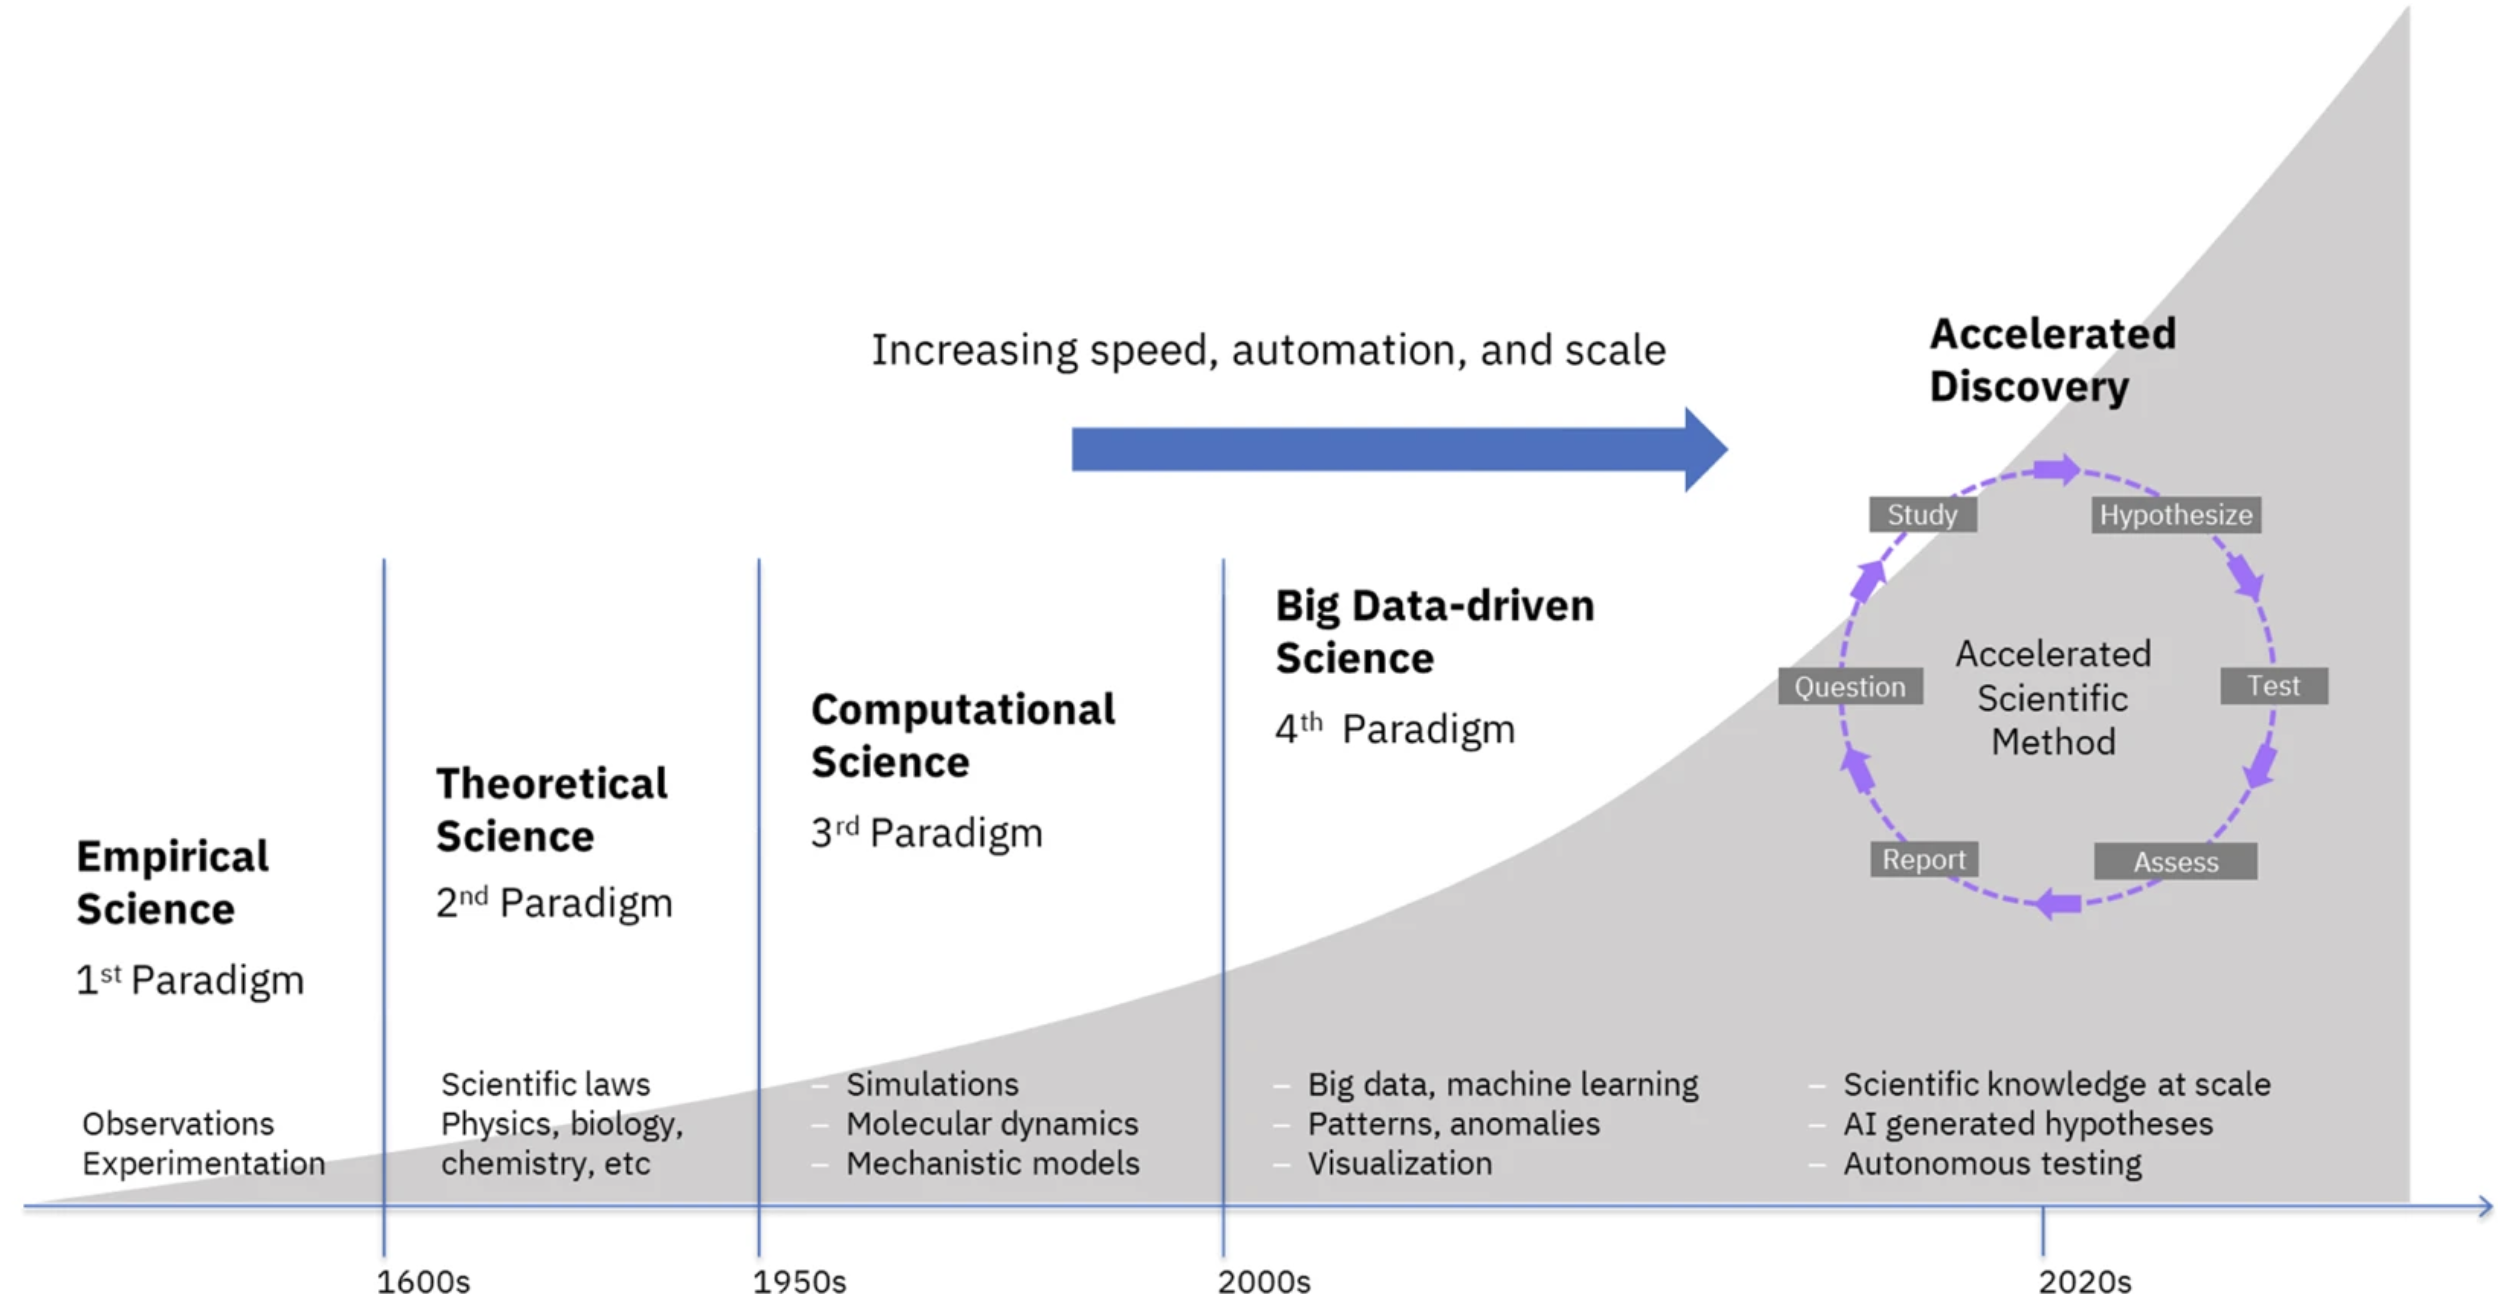
\includegraphics[width=\textwidth]{figures/literature-review/figure2-1.png}
    \caption{The four paradigms of scientific discovery\cite{RN448}.}
    \label{fig:figure2.1}
\end{figure}

The applications of AI in materials science are diverse and rapidly expanding. AI serves as an overarching framework encompassing various concepts, with machine learning (ML) as a key subset specifically applied to materials science. At its core, ML is utilized to identify complex relationships that are either too intricate or computationally expensive for traditional analytical methods\cite{RN318}. Key applications include: 

\begin{enumerate}
  \item Learning structure-property relationships: ML models can predict material properties directly from structural information\cite{RN580,RN556,RN533}. For example, deep learning models have been employed to learn the relationship between the structure of organic molecules encoded in fingerprints and their emission characteristics in light-emitting diodes\cite{RN66}. For inorganic materials, deep learning model has been used to model the relationship between the composition of high-entropy alloys and their thermal expansion coefficients\cite{RN532}. 
  
  \item Optimizing synthesis parameters: AI can elucidate reaction mechanisms and optimize experimental conditions for complex chemical reactions\cite{,RN341,RN574,RN552,RN581}. Supervised ML models have been trained to correlate synthesis parameters with reaction outcomes, enabling the efficient design of experiments and reducing the trial-and-error typically associated with materials synthesis\cite{RN328}. 
  
  \item Accelerating computational methods: AI models can reduce the computational cost of traditional simulation techniques. For instance, active learning models have been developed to perform quantum mechanical calculations using small to medium-sized molecular building blocks instead of individual atoms, as in first-principles methods. These models have demonstrated faster and reliable predictions across diverse material systems and target properties\cite{RN561}.
  
\end{enumerate}

Given the broad range of AI applications in materials science, this literature review chapter focuses specifically on machine learning for materials discovery. This domain often encompasses one or more of the scenarios discussed above, with the primary goal of identifying novel or previously unexplored materials that exhibit superior properties compared to existing ones. In the following sections, we provide a systematic framework to clarify the various ML methods employed in materials discovery, addressing the diverse terminologies commonly found in the literature. Additionally, we will discuss how these ML methods can be integrated into a comprehensive machine learning workflow and how they can be effectively combined with other data-driven approaches to enhance materials research.




\subsection{Types of ML methods used for materials discovery}

\begin{figure}[ht]
    \centering
    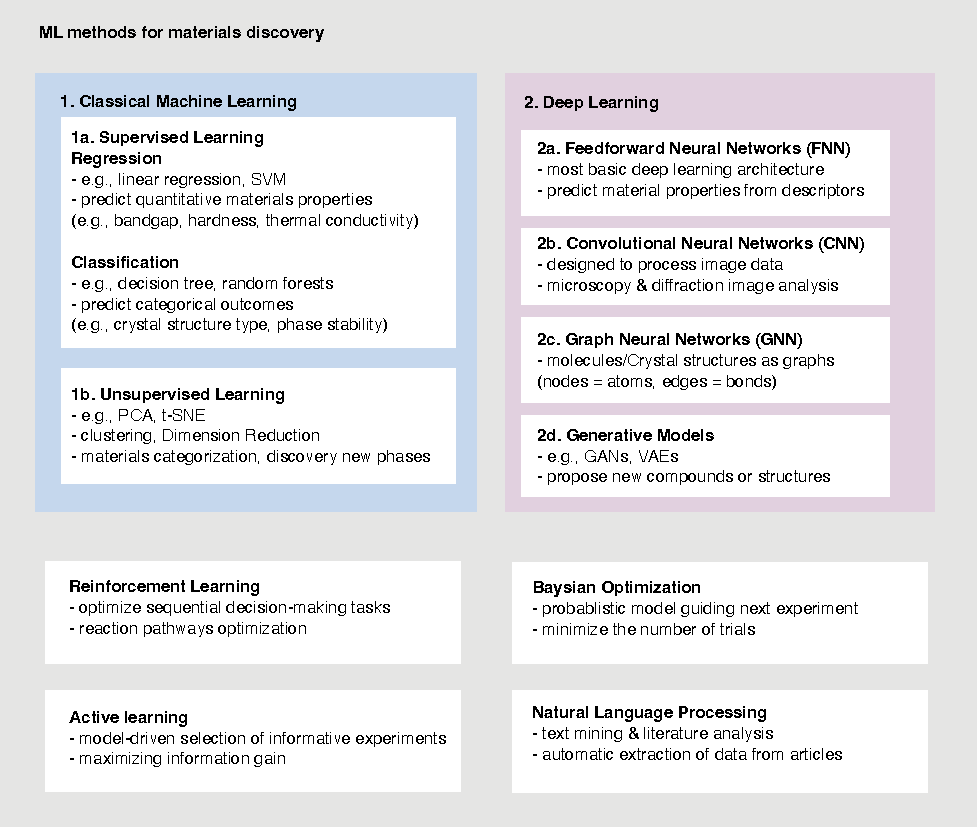
\includegraphics[width=\textwidth]{figures/literature-review/figure2-2.pdf}
    \caption{Common types of ML methods typically used in materials science.}
    \label{fig:figure2.2}
\end{figure}

An overview of commonly used ML methods is summarized in Figure \ref{fig:figure2.2}. Within ML, approaches that rely on manually engineered features and relatively simple model architectures are referred to as classical ML methods, with supervised learning being one of the earliest and mostly widely used techniques. The first notable application of supervised learning in materials science dates back to 2010, where a probabilistic model is built to identify the most probable crystal structures of unseen ternary oxide compounds\cite{RN542}. Classical ML methods remain widely used, particularly when dealing with smaller datasets (typically below thousands of data points) or when model interpretability is a key priority. Meanwhile, deep learning represents a specialized branch of ML that employs multi-layered neural networks capable of automatically extracting features from raw data. Unlike classical ML methods, deep learning does not require manual feature engineering, as it can learn hierarchical representations directly from input data. Deep learning methods have become increasingly popular in materials science due to their superior performance in tasks involving large and high-dimensional datasets. However, DL methods typically require larger datasets (often exceeding $\sim10,000$ data points), significant computational resources, and can be less interpretable compared to classical ML approaches.

\textbf{Classical Machine Learning}

The most distinctive types of classical ML methods are supervised and unsupervised learning.
In supervised learning, models are trained on labelled datasets, where each data point is associated with a known outcome, such as a material property (for regression tasks) or a class label (for classification tasks). 
\begin{itemize}
    \item Regression models, such as linear regression, random forests, Gaussian process regression, and support vector regression (SVR), are used to map input descriptors (e.g., elemental fractions, lattice parameters) to quantitative material properties such as bandgap, thermodynamic stability, and morphology\cite{RN563,RN593,RN317,RN13}. For instance, a random forest regression model has been employed to correlate the elemental composition of adsorption sites with the electrocatalytic adsorption energy of copper-containing intermetallic crystals\cite{RN551}. 

    \item Classification techniques such as logistic regression, support vector machines (SVMs), decision trees are designed to predict discrete labels. These models are commonly applied to tasks such as phase classification, crystal structure identification, and synthesizability prediction\cite{RN315,RN580,RN321}. For example, various classification models have been used to distinguish between different oxidation states in metal-organic frameworks (MOFs) based on local environmental features, including metal type, coordination geometry, and chemical environment\cite{RN580}.
    
\end{itemize}

Supervised learning approaches excel when reliable labelled data is available, whether from experimental measurements or computational simulations. They are typically more interpretable and computationally efficient compared to many deep learning models, making them attractive for iterative property prediction and materials design workflows.

In unsupervised learning, the objective is to uncover hidden patterns or groupings within unlabelled data without predefined outcomes. 

\begin{itemize}
    \item Clustering algorithms like k-means clustering, hierarchical clustering, and Gaussian mixture models are employed to group materials with similar feature profiles, potentially revealing unexpected trends or novel material families\cite{RN571,RN555}. For example, a study applied hierarchical agglomerative clustering to categorize ternary nitrides into distinct chemical families based on their stability and metastability profiles\cite{RN555}.
    \item Dimensionality reduction techniques, including principal component analysis (PCA) and t-distributed stochastic neighbour embedding (t-SNE), are used to project high-dimensional materials data into lower-dimensional spaces. This facilitates the visualization of patterns, identification of outliers, and discovery of structure–property relationships that might be obscured in higher dimensions\cite{RN412,RN574,RN551}.
\end{itemize}

By revealing latent structures in the data, unsupervised methods can provide valuable insights into structure–property correlations and guide targeted experimental or computational investigations.

\textbf{Deep Learning}

Deep learning (DL) is a specialized branch of ML that employs multi-layered neural networks to automatically learn features from raw data. This approach significantly reduces the need for manual feature engineering, provided that sufficient training data and computational resources are available. DL models excel at capturing complex, non-linear relationships in high-dimensional datasets, making them particularly valuable for a wide range of materials science applications.

Feedforward neural networks (FNNs) represent the most basic form of deep learning architecture. In these models, information flows in a single direction—from input to output—through multiple layers of interconnected nodes (neurons). FNNs are effective for both regression and classification tasks, particularly when datasets are large enough to support the direct learning of representations from raw inputs, such as the chemical structures of organic molecules\cite{RN581,RN610}. In one of the earliest applications of deep learning in materials science, a simple neural network architecture with two hidden layers—the minimum number required to be classified as deep learning—was used to design organic molecules for light-emitting diode (LED) applications\cite{RN66}. While more advanced deep learning architectures have since been developed, FNNs are often employed as baseline models for benchmarking the performance of more complex networks.

Convolutional neural networks (CNNs) are designed to process grid-like data structures, such as images, by applying convolutional filters that automatically detect spatial hierarchies and local patterns. In materials science, CNNs are widely used for analysing image-based datasets, including microscopy images (e.g., SEM, TEM) to identify microstructural features or defect distributions and diffraction patterns for automated phase classification and structural analysis\cite{RN550,RN604,RN564}. For example, a CNN architecture with six convolutional layers was developed to classify crystal phases from X-ray diffraction (XRD) patterns automatically\cite{RN604}.

Graph neural networks (GNNs) are particularly well-suited for materials science because they natively process graph-structured data, which naturally represents molecules and crystal structures. In this framework, atoms are represented as nodes, and bonds or interatomic interactions are represented as edges. GNNs have demonstrated remarkable success in predicting a wide range of material properties, including crystal stability, electronic properties, and surface chemistry\cite{RN336,RN562,RN362}. A notable example is GNoMe, a state-of-the-art AI model developed by Google DeepMind, which uses GNNs to predict and discover new crystalline materials. GNoMe has achieved unprecedented scalability, significantly improving the efficiency of materials discovery—reportedly accelerating the process by an order of magnitude\cite{RN601}.

Generative models aim to create new data samples that resemble the distribution of existing data, making them highly effective for inverse materials design. Two widely used generative models in materials science include Generative Adversarial Networks (GANs) and Variational Autoencoders (VAEs). Generative models can propose novel materials with desired properties, such as targeted band gaps, thermal conductivity, or mechanical strength\cite{RN326,RN532,RN412}. For instance, MatterGen, a generative AI model developed by Microsoft Research, represents a significant breakthrough in materials science\cite{RN633}. It enables the design of new inorganic materials with specific target properties, greatly accelerating the exploration of vast compositional spaces.

\textbf{Other Machine Learning Methods}

Active learning is especially valuable when experimental or simulation data are scarce or expensive to obtain. In this method, the model autonomously selects the most informative data points or experiments to label next, thereby optimizing the learning process with minimal resources. Active learning strategies are often integrated with Gaussian process regression (GPR), due to its inherent uncertainty quantification, or neural networks to target high-uncertainty regions in the materials design space. This approach rapidly converges on optimal candidates while minimizing total experimental cost\cite{RN601, RN604, RN551,RN532}.

In contrast to methods that rely on static datasets, reinforcement learning (RL) focuses on sequential decision-making, where an agent explores chemical or process pathways and receives “rewards” for achieving specific outcomes (e.g., synthesizing a stable or high-performing material). RL is particularly powerful in dynamic laboratory environments, enabling autonomous experimentation through real-time tuning of synthesis parameters and adaptive control of reactors. This exploration-exploitation framework allows RL to discover novel materials and optimize processes beyond human intuition\cite{RN604,RN339}.
Bayesian optimization employs probabilistic models to iteratively recommend the next most promising experiments based on current knowledge and uncertainty. By leveraging acquisition functions—such as expected improvement or upper confidence bound—these methods balance exploration and exploitation to efficiently identify parameter sets or compositions with superior properties (e.g., optimized reaction yield or solar cell efficiency)\cite{RN549,RN362,RN612}.

Natural language processing (NLP) facilitates large-scale text mining of scientific literature, patents, and databases to extract valuable information, including synthesis protocols, property data, and structure-property relationships. Recent advances, particularly transformer-based models, have enhanced the ability to capture complex semantic patterns. When combined with knowledge graph construction, NLP can reveal hidden correlations, accelerate hypothesis generation, and guide experimental design toward previously unexplored materials spaces\cite{RN604,RN635,RN634,RN636}.

\subsection{Incorporation into Materials Discovery Workflows}

\begin{figure}[ht]
    \centering
    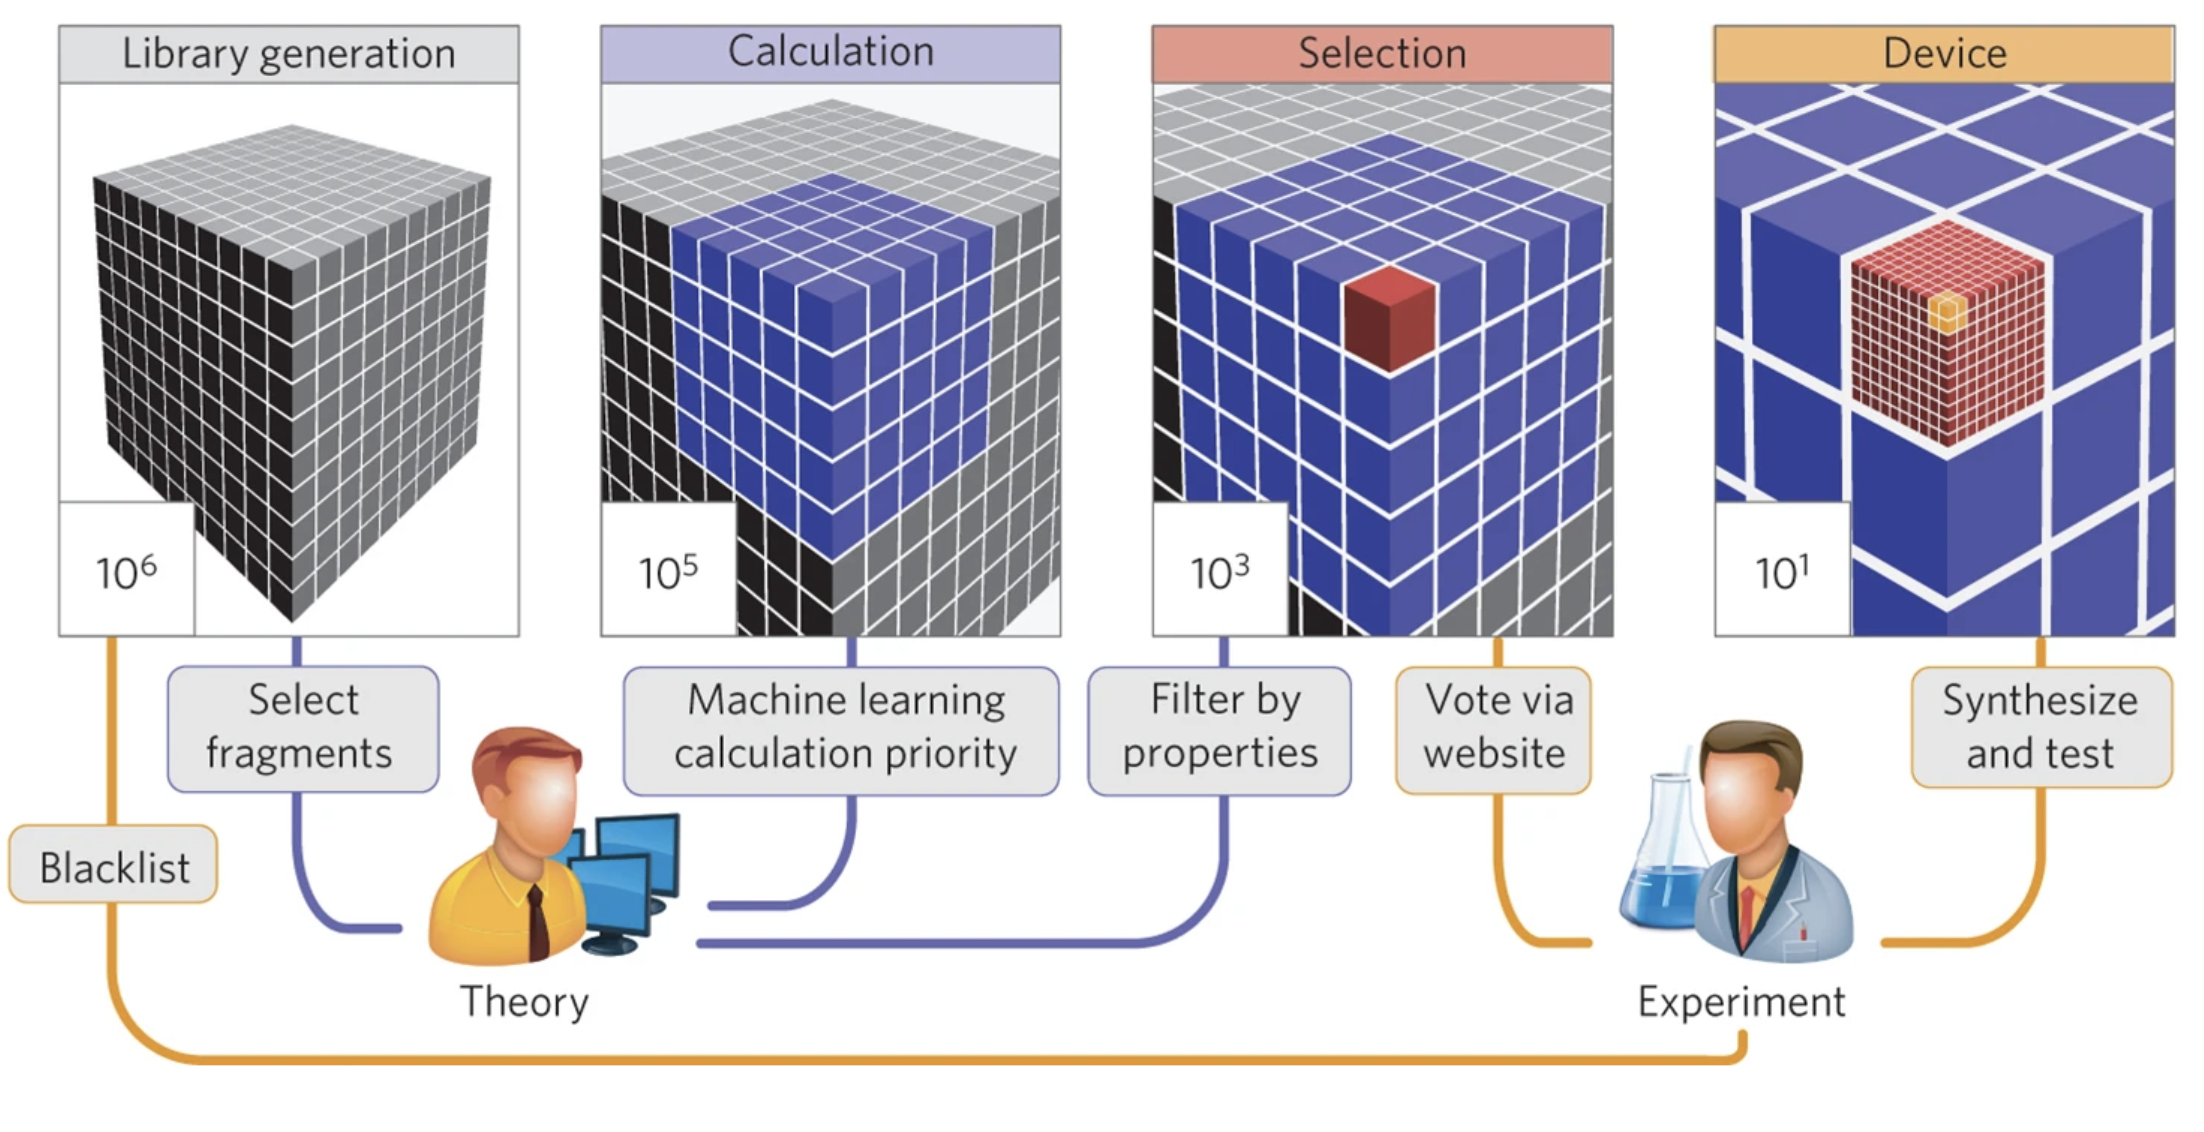
\includegraphics[width=\textwidth]{figures/literature-review/figure2-3.png}
    \caption{A ML-assisted materials discovery workflow in an early OLED study\cite{RN66}.}
    \label{fig:figure2.3}
\end{figure}

Building on the discussion of ML methods used in materials discovery, this section explores how ML is seamlessly integrated into materials discovery pipelines. Since ML models require large datasets to learn effectively, they are often combined with high-throughput computational tools and experimental platforms to generate the necessary training data.

On the computational side, large-scale density functional theory (DFT) and molecular dynamics (MD) simulations serve as key sources of labelled datasets for ML model training and fine-tuning. These simulations help establish structure–property relationships, enabling models to make more accurate predictions. Meanwhile, on the experimental side, automated synthesis and characterization platforms generate high-quality data that can be continuously fed back into ML models. This iterative process forms a closed-loop system where predictions guide experiments, and experimental outcomes, in turn, refine the model, accelerating the materials discovery cycle.

One of the earliest examples of ML integration in materials discovery was demonstrated in a 2016 study on organic light-emitting diode (OLED) materials\cite{RN66}. In this work, a simple deep learning model with just two hidden layers was incorporated into a materials discovery workflow that included materials generation, high-throughput calculations, virtual screening, and experimental fabrication (Figure \ref{fig:figure2.3}). This streamlined workflow identified thousands of promising candidates, and subsequent experimental validation revealed several materials with exceptionally high quantum efficiency, showcasing the predictive power and practical utility of ML-enhanced discovery pipelines.

\begin{figure}[ht]
    \centering
    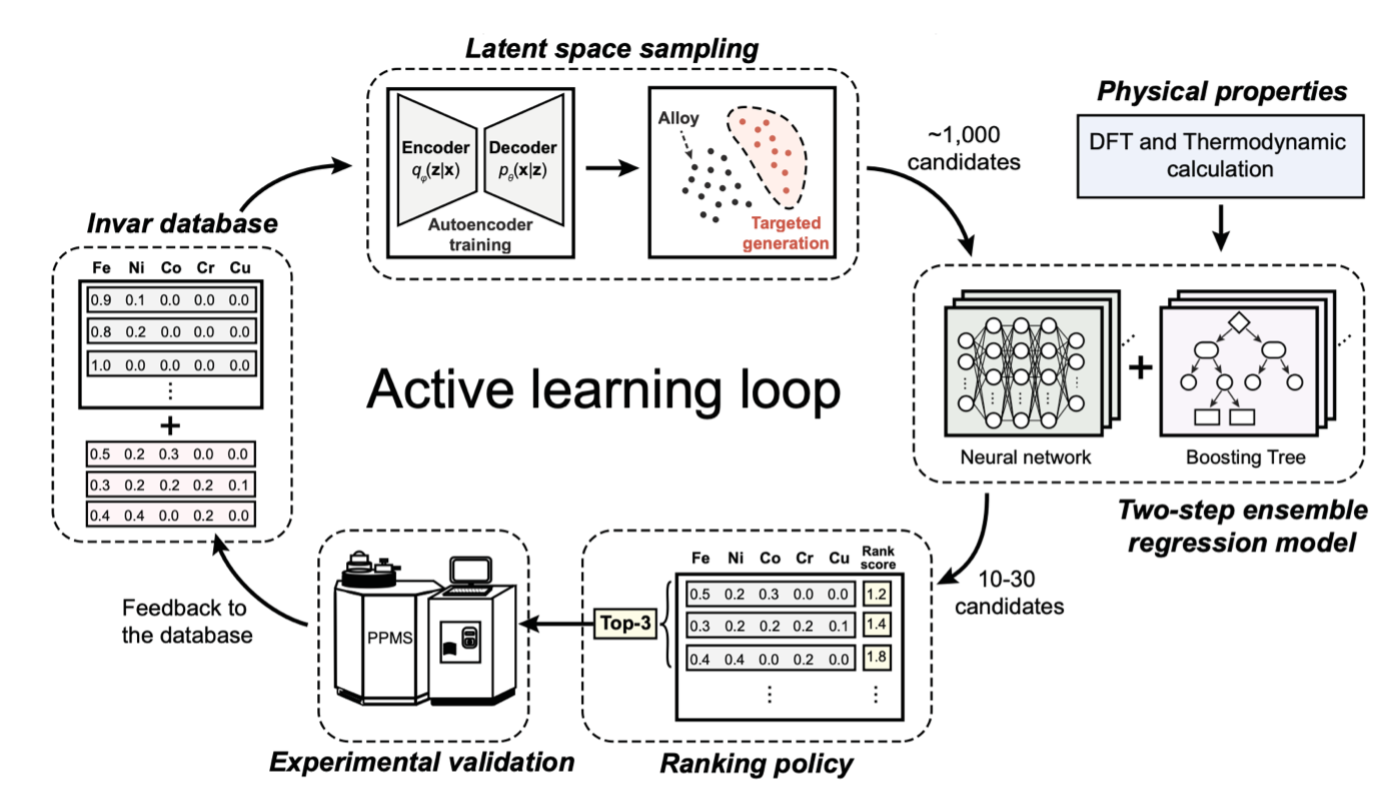
\includegraphics[width=\textwidth]{figures/literature-review/figure2-4.png}
    \caption{An active learning loop applied to high-entropy alloy discovery\cite{RN532}.}
    \label{fig:figure2.4}
\end{figure}

A more advanced example is the discovery of high-entropy alloys (HEAs) as shown in Figure \ref{fig:figure2.4}, where an active learning framework was developed, integrating ML with high-throughput DFT calculations, thermodynamic modelling, and experimental synthesis\cite{RN532}. At the core of this workflow, a generative model proposed new compositions, while a custom two-step regression model predicted their properties. Out of millions of potential compositions, 17 new alloys were synthesized and characterized, leading to the identification of two HEAs with targeted thermal expansion properties.


\begin{figure}[ht]
    \centering
    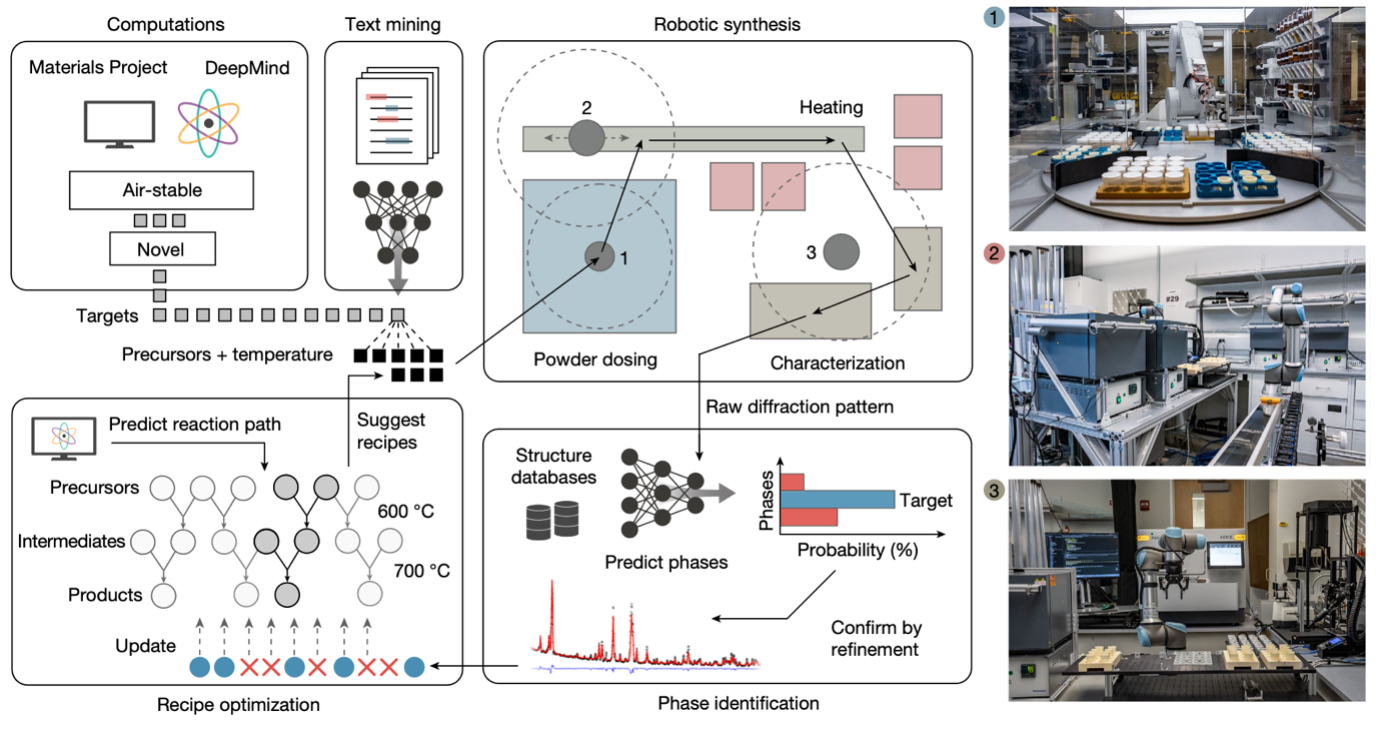
\includegraphics[width=\textwidth]{figures/literature-review/figure2-5.png}
    \caption{Automated materials discovery with the A-Lab platform\cite{RN604}.}
    \label{fig:figure2.5}
\end{figure}

At the highest level of complexity, fully autonomous materials discovery systems are emerging, integrating multiple AI models into unified closed-loop frameworks. A notable example is the A-Lab platform (Figure \ref{fig:figure2.5}), which employs several ML models to accelerate discovery\cite{RN604}. First, an NLP model is trained on extensive databases of synthesis procedures extracted from the literature. This is followed by a regression model that predicts optimal synthesis temperatures based on precursor materials. When initial synthesis attempts are unsuccessful, an active learning algorithm iteratively refines the synthesis parameters using experimental feedback. Finally, convolutional neural networks (CNNs) are employed to analyse X-ray diffraction (XRD) patterns of the synthesized materials, aiding in the rapid identification of successful synthesis outcomes.

\subsection{Inverse Design in Materials Discovery}

\begin{figure}[ht]
    \centering
    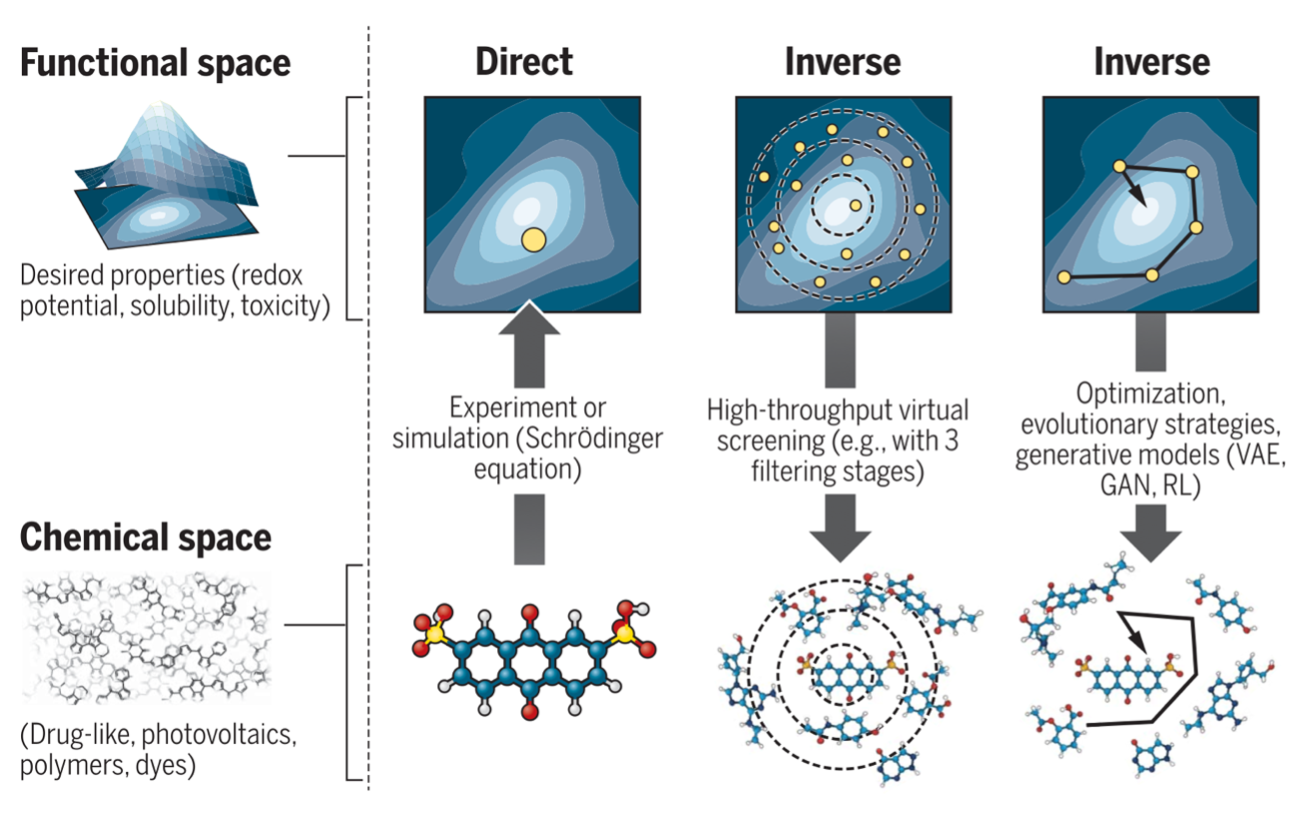
\includegraphics[width=\textwidth]{figures/literature-review/figure2-6.png}
    \caption{Overview of direct and inverse approaches in materials discovery\cite{RN361}.}
    \label{fig:figure2.6}
\end{figure}

Building upon the integration of ML into materials discovery workflows, an even more ambitious application is inverse design, often regarded as a significant milestone—or even the “holy grail”—of materials discovery. Rather than adopting the traditional forward or direct-design approach of starting with a known material and then determining its properties, inverse design begins by specifying target properties or functionalities (Figure \ref{fig:figure2.6}). Computational methods are then used to identify, generate, or suggest materials that fulfill these specifications. This property-oriented framework is poised to efficiently traverse the vast chemical and structural space, thereby minimizing trial-and-error experimentation and accelerating the discovery of novel materials with precise functionalities\cite{RN361,RN547}.

Although the concept of inverse design has been discussed for several decades, the rapid rise of ML in materials science has significantly advanced its practical implementation. Thanks to ML’s capacity to model high-dimensional data and capture complex structure–property relationships, inverse design workflows have become more robust and predictive, offering the potential for real-world applicability in diverse materials domains.

Despite its growing popularity, inverse design does not yet have a universally agreed-upon definition within the materials science community. Some methodologies that effectively implement an inverse design workflow do not explicitly label themselves as such. For instance, while high-throughput screening (HTS) is often considered part of forward discovery, some researchers classify it as a subset of inverse design. These terminological distinctions highlight the evolving nature of the field, but the fundamental principle of inverse design remains unchanged: instead of starting with a known material and analysing its properties, we begin with a desired property and work backward to identify suitable structures or compositions. 

Three primary methodologies are commonly used in inverse design: (1) generative models, (2) iterative design strategies (e.g., active learning, Bayesian optimization, genetic algorithms), and (3) invertible materials representations. Among these, generative models and invertible representations take a fundamentally different approach from iterative techniques. While iterative methods refine candidate materials through sequential optimization loops, generative models and invertible representations aim to construct viable materials from scratch based on predefined target properties. By leveraging these approaches, researchers can efficiently explore vast chemical spaces and propose entirely new material candidates, rather than incrementally improving known ones. This ability to generate novel structures directly from property requirements makes these methods particularly valuable for inverse design. The following sections provide an in-depth overview of generative models and invertible materials representations, examining their respective strengths, limitations, and distinct roles in accelerating materials discovery.

\begin{figure}[ht]
    \centering
    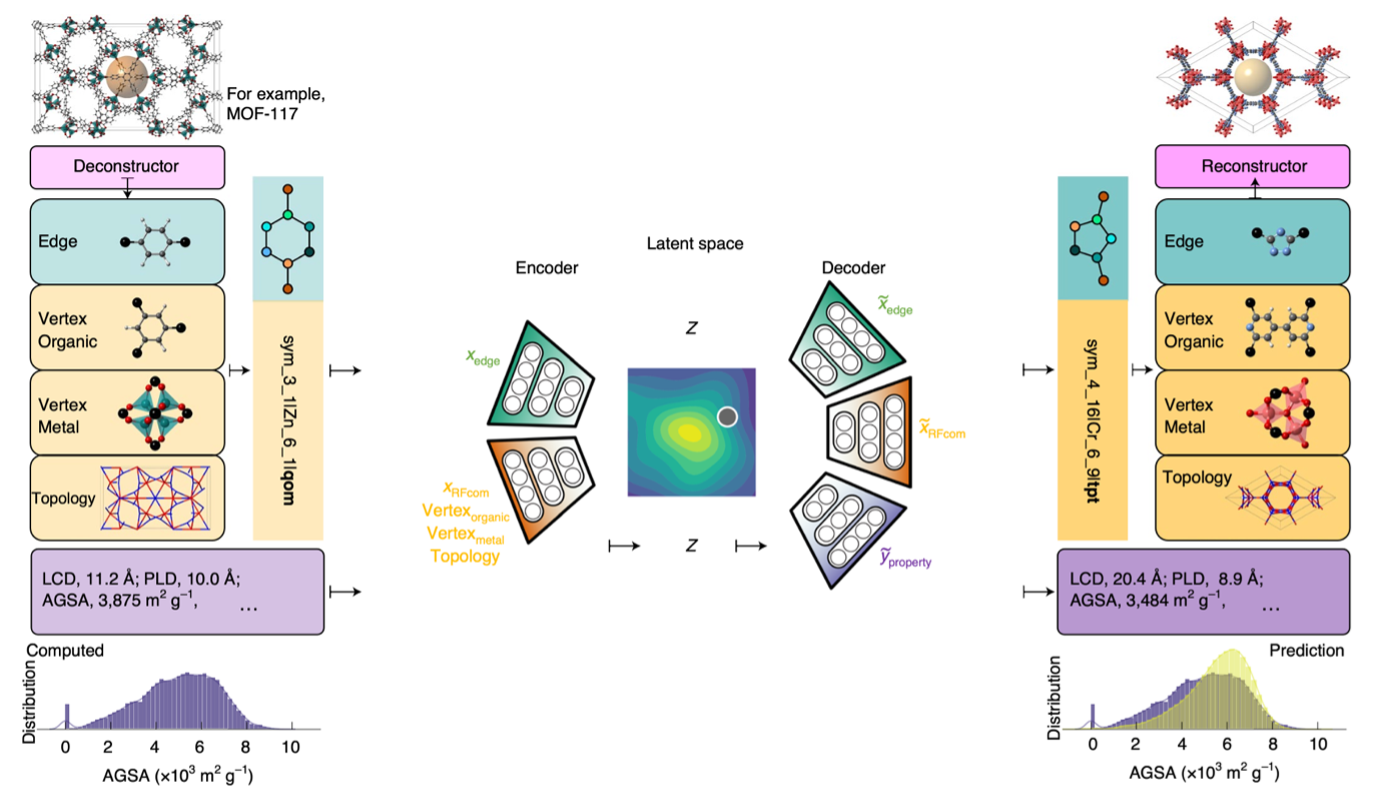
\includegraphics[width=\textwidth]{figures/literature-review/figure2-7.png}
    \caption{Schematic representation of a typical generative model workflow\cite{RN412}.}
    \label{fig:figure2.7}
\end{figure}

\textbf{Generative models}

Generative models including Variational Autoencoders (VAEs) and Generative Adversarial Networks (GANs), have emerged as powerful techniques for inverse design\cite{RN412, RN633, RN347, RN614, RN70}. In these frameworks, models learn probabilistic distributions over existing materials or molecules. Once trained, they can generate new candidate structures or compositions that are likely to exhibit desired properties, effectively “mapping” targeted characteristics back to plausible chemical formulas or structural motifs. These methods are particularly impactful in organic molecule design (e.g., pharmaceuticals, organic semiconductors), where a dense, high-quality dataset of known molecules can be leveraged to yield innovative new candidates. 

One of the earliest notable demonstrations of a generative model in materials discovery was a VAE architecture composed of an encoder and decoder using recurrent neural networks, designed to generate organic molecules\cite{RN411}. Since then, generative models have been applied across various material classes. For example, they have been used to generate novel metal–organic frameworks (MOFs) with exceptional gas separation properties\cite{RN412}. More recently, MatterGen, a generative model introduced by Microsoft, has demonstrated the ability to generate stable and diverse inorganic materials spanning the entire periodic table. Moreover, it can be fine-tuned to design materials with specific target properties\cite{RN633}. 

Despite these successes, the application of generative models remains largely limited to material classes with relatively well-defined structures and abundant training data. Their implementation in highly constrained materials systems, such as the organic spacers in 2D perovskites, is still rare. This limitation may stem from the scarcity of high-quality datasets in these domains, which restricts the model’s ability to learn meaningful structure–property relationships. Without sufficient domain knowledge or physics-based constraints integrated into the learning process, generative models struggle to propose viable candidates in these more complex materials spaces. Addressing these challenges will be crucial for expanding the scope of inverse design methodologies to a broader range of materials.

\textbf{Invertible Material Representations}

A growing area of research focuses on developing bidirectional mappings between material representations and desired property spaces\cite{RN354,RN599}. Unlike many black-box models that learn an inverse mapping implicitly, invertible representations provide a more transparent and structured approach to inverse design. This enables researchers to start in the property domain and systematically work backward to identify candidate structures, making the design process more interpretable and controllable. For molecular systems, several well-established invertible representations exist, including simplified molecular-input line-entry system (SMILES), international Chemical Identifier (INCHI) and molecular graph\cite{RN648}. These representations allow machine learning models to efficiently encode molecular structures and generate new candidates based on specified properties. 

\begin{figure}[ht]
    \centering
    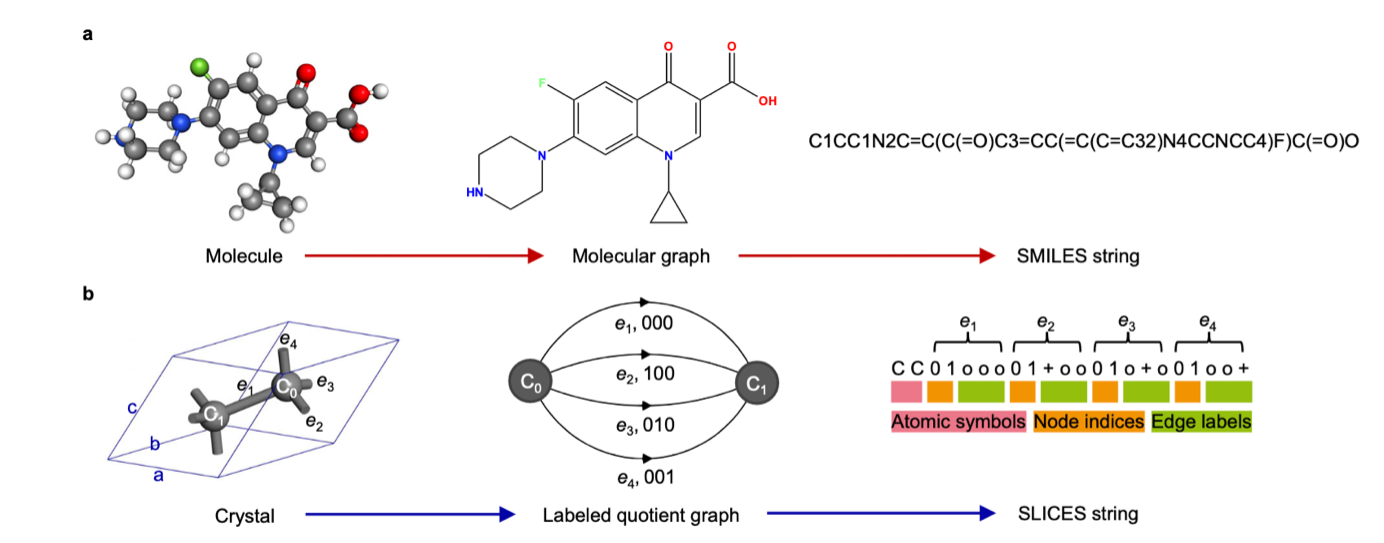
\includegraphics[width=\textwidth]{figures/literature-review/figure2-8.png}
    \caption{Invertible representations in molecular systems and solid-state crystals\cite{RN642}.}
    \label{fig:figure2.8}
\end{figure}

For inorganic crystals, the development of invertible representations is more challenging. Unlike molecules, where connectivity can be described in a straightforward manner, solid-state materials require a representation that captures both periodicity and compositional complexity. This has been a longstanding challenge in materials informatics, as achieving invertibility while maintaining generalizability and property-driven design remains difficult. Several representations have been proposed to address this issue, but none have yet become universal standard\cite{RN642,RN354}.

Despite these challenges, invertible material representations have significant potential in inverse design, particularly when used in conjunction with machine learning models. By establishing structured and reversible mappings between materials and their properties, these representations provide a powerful framework for rational material generation, facilitating more efficient and targeted discovery.

\section{2D Hybrid Perovskites}\label{section:section2-2}

Two-dimensional (2D) hybrid perovskites have emerged as a fascinating class of materials that combine the desirable optoelectronic properties of their three-dimensional counterparts with enhanced chemical and environmental stability. In general, these materials consist of inorganic metal halide layers separated by organic cations, creating a naturally layered architecture. By tuning the thickness of these inorganic layers or altering the organic interlayers, researchers can tailor properties such as bandgap, exciton binding energy, and overall structural stability. Thus, 2D perovskites have attracted attention for applications ranging from solar cells and light-emitting diodes to photodetectors and field-effect transistors\cite{RN108}.

Unlike 3D perovskites, where small organic cations (e.g., methylammonium or formamidinium) fit within the perovskite lattice, 2D perovskites incorporate larger organic spacer molecules that enforce a layered structure and introduce new functionalities. This dimensional reduction results in strong quantum confinement effects, leading to distinct optical and electronic behaviours compared to their 3D analogy. In the following subsections, we discuss the structural variations of 2D perovskites, focusing on key phase families, and explore their fundamental electronic properties.

\subsection{Structural and Electronic Fundamentals}

\begin{figure}[ht]
    \centering
    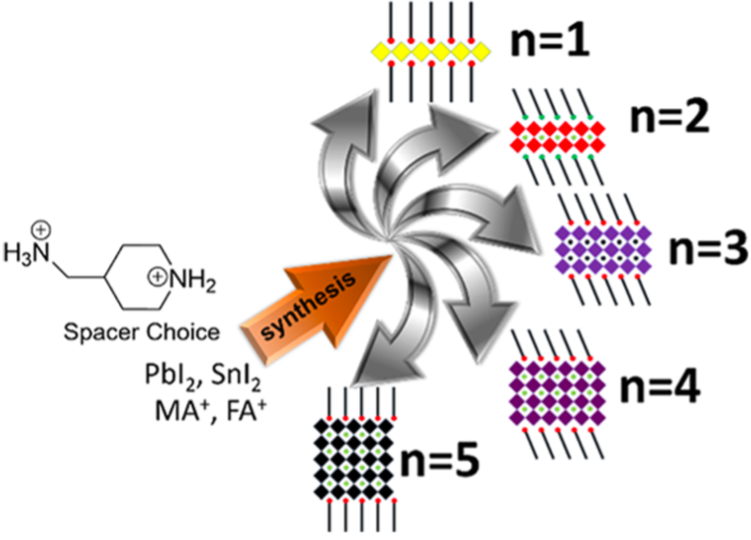
\includegraphics[width=0.6\textwidth]{figures/literature-review/figure2-9.png}
    \caption{Design strategy for organic spacers in 2D perovskites\cite{RN144}.}
    \label{fig:figure2.9}
\end{figure}

\textbf{Structural fundamentals}

2D perovskites exhibit rich structural diversity, primarily arising from variations in both the inorganic metal-halide framework and the organic spacers\cite{RN394}. The inorganic layers are composed of corner-sharing metal halide octahedra, which can stack to form structures ranging from single-layered (strictly 2D perovskites, n = 1) to multi-layered (quasi-2D perovskites, n > 1)\cite{RN140}. As the number of inorganic layers approaches infinity (n → ∞), the structure converges to that of a 3D perovskite. Additionally, the metal (e.g., Pb, Sn) and halide (e.g., I, Br, Cl) compositions in the inorganic framework can be tuned, with large chemical space available\cite{RN102}. Meanwhile, the organic spacer cations play a pivotal role in determining the exact structural phase (Figure \ref{fig:figure2.10}), giving rise to three main families of 2D perovskites: Ruddlesden–Popper (RP), Dion–Jacobson (DJ), and Alternating Cation-Interlayer (ACI).

\begin{figure}[ht]
    \centering
    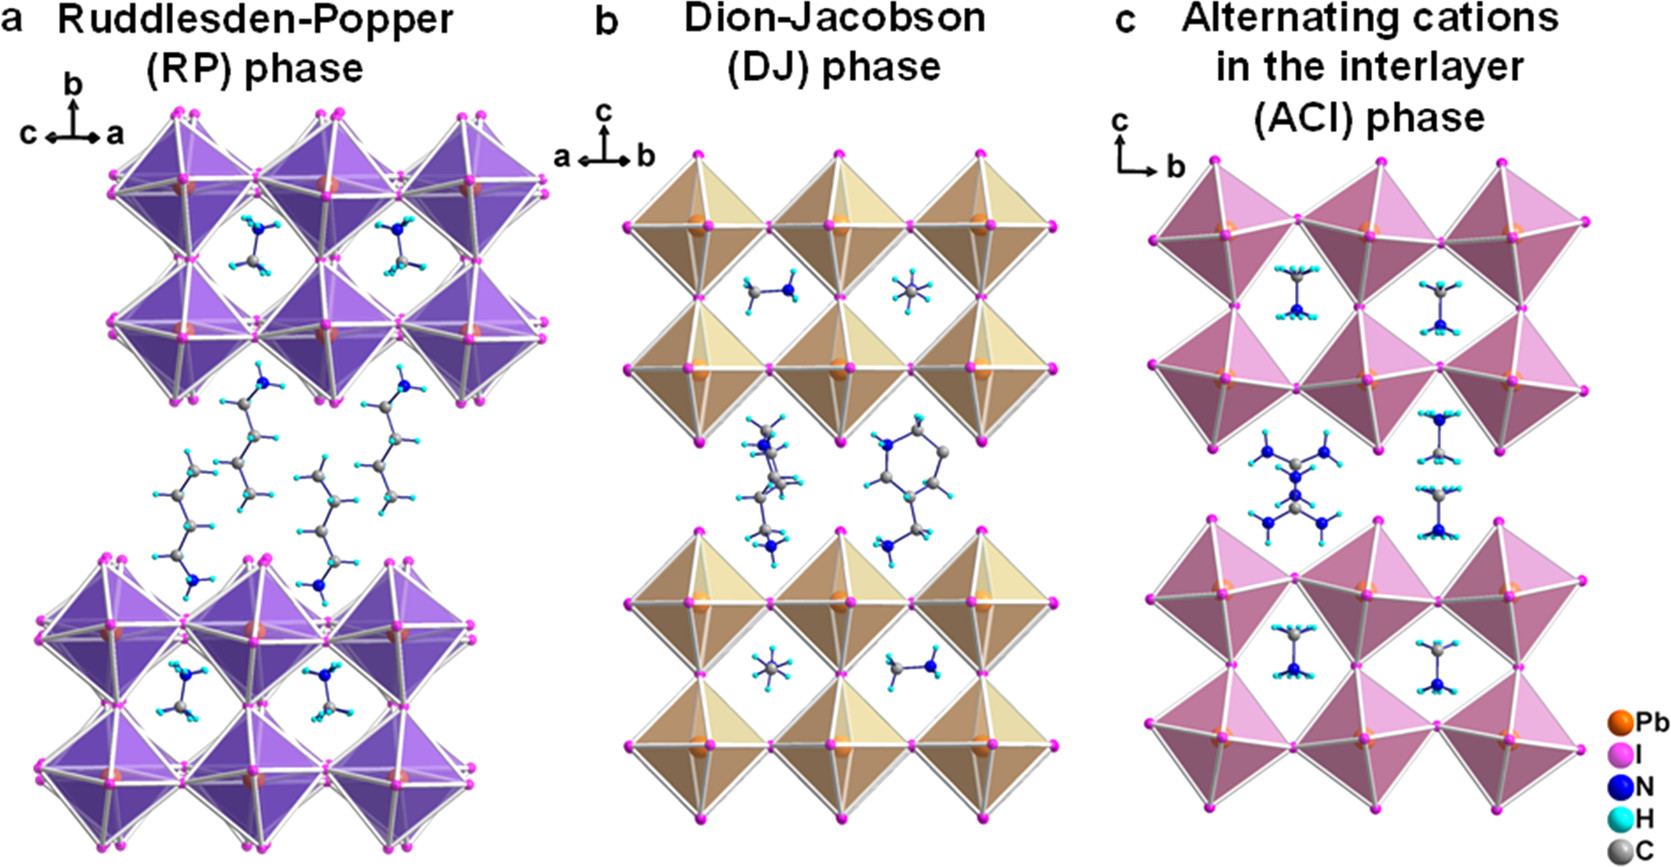
\includegraphics[width=0.9\textwidth]{figures/literature-review/figure2-10.png}
    \caption{Schematic illustration of different structural phases of 2D perovskites\cite{RN144}.}
    \label{fig:figure2.10}
\end{figure}

The \textbf{RP phase} represents the most extensively studied family of 2D perovskites and can be described by the general formula (A’)$_2$A$_{n-1}$M$_n$X$_{3n+1}$. Here, A′ is a bulky monovalent organic spacer cation, A is a smaller monovalent cation (as seen in 3D perovskites), M is a metal cation (e.g., Pb$^{2+}$, Sn$^{2+}$), and X is a halide anion. Two layers of organic spacers intercalate between the inorganic slabs, creating a van der Waals gap. While many RP-phase perovskites display an in-plane octahedral shift of (1/2, 1/2), more complex tilts and distortions can occur with bulky or flexible organic spacers. Despite potential drawbacks—such as restricted out-of-plane transport due to the van der Waals gap—RP perovskites are valued for their strong excitonic effects, tunable bandgaps, and suitability for light-emitting and photodetection applications\cite{RN108,RN190}.

The \textbf{DJ phase}, described by the formula A’A$_{n-1}$M$_n$X$_{3n+1}$, where A’ is typically a divalent organic spacer cation (e.g., diammonium compounds) with two ammonium tethering groups anchor to the inorganic layers. In contrast to the RP phase, DJ perovskites have only a single organic spacer layer between inorganic slabs, thus eliminating the van der Waals gap and often reducing the interlayer distance\cite{RN106}. This configuration improves out-of-plane electronic coupling and charge transport while strengthening hydrogen-bonding interactions—leading to excellent structural stability. Such attributes render DJ perovskites promising candidates for high-efficiency solar cells and transistors\cite{RN198}. 

The \textbf{ACI phase} is a relatively new structural motif where two different organic cations alternate between the inorganic layers, with the first example demonstrated in 2017\cite{RN214}. Often, the organic spacer cations are relatively small (comparable to methylammonium), resulting in shorter interlayer distances and stronger interlayer coupling\cite{RN242}. This structural motif can yield a reduced bandgap and enhanced charge transport, and there have been demonstrations of improved solar-cell efficiencies over comparable RP and DJ phases\cite{RN212,RN208}. However, because of stricter size constraints on the organic cations, the chemical space for ACI-phase perovskites is comparatively smaller.


\begin{figure}[ht]
    \centering
    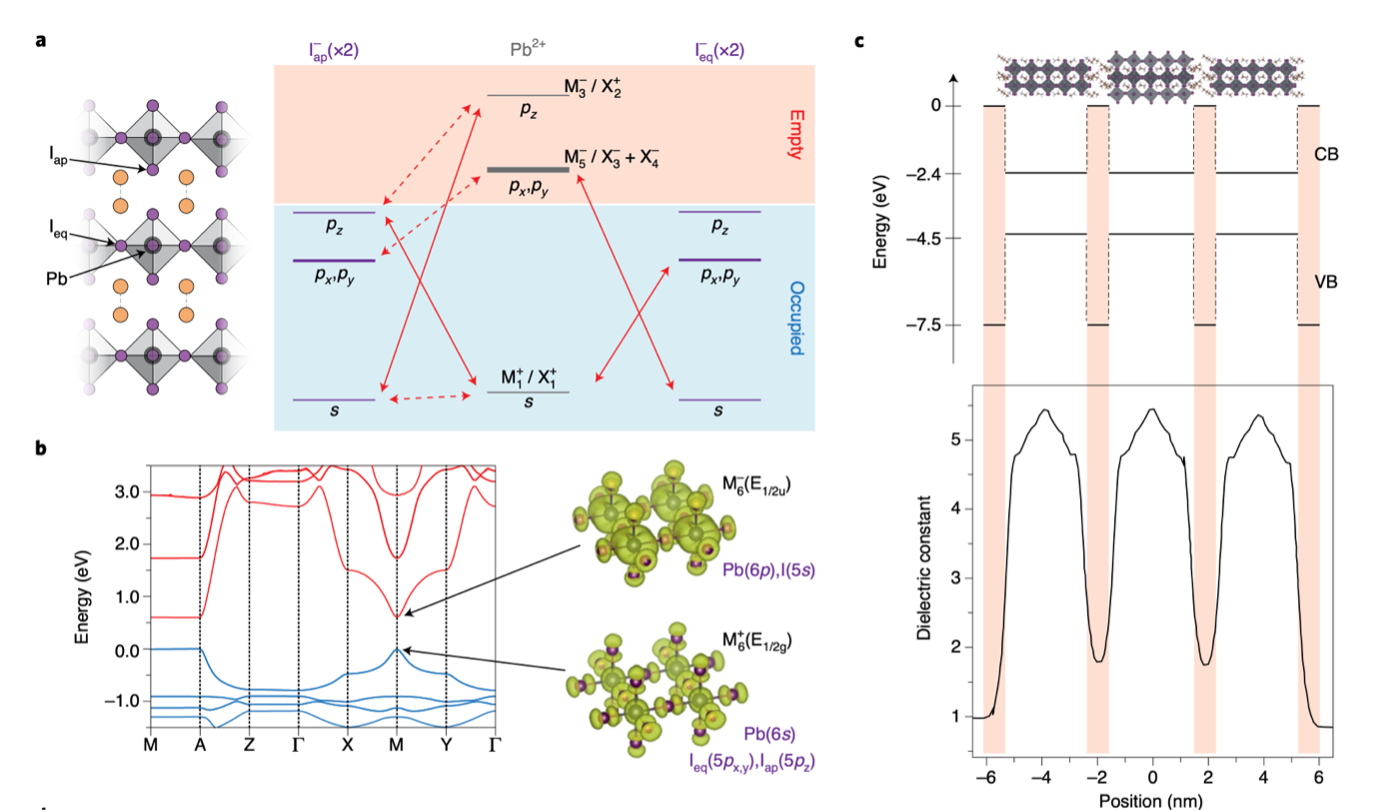
\includegraphics[width=\textwidth]{figures/literature-review/figure2-11.png}
    \caption{Electronic properties of 2D perovskites\cite{RN119}.}
    \label{fig:figure2.11}
\end{figure}

\textbf{Electronic Fundamentals}

The electronic structure of 2D perovskites is now relatively well understood, with their band edges predominantly governed by the inorganic layers and their structural and dielectric environment modulated by the organic spacers (Figure \ref{fig:figure2.11}). 

Generally, the bandgap widens as the thickness of the inorganic layer decreases (i.e., as n decreases). For example, monolayer (n = 1) perovskites typically exhibit bandgaps $\sim2.4$ eV, while quasi-2D structures with larger n values approach the bandgap of the corresponding 3D perovskite ($\sim1.5$ eV for MAPbI$_3$)\cite{RN199}. This tunability has been leveraged in studies to induce an “energy funneling” effect, where charge carriers move from wider-bandgap (lower-n) to narrower-bandgap (higher-n) regions, enhancing the efficiency of light-emitting diodes\cite{RN180}. Beyond structural thickness, the bandgap can also be finely tuned by altering the metal cation (M = Pb$^{2+}$, Sn$^{2+}$) or halide anion (X = I$^-$, Br$^-$, Cl$^-$)\cite{RN104}.



A defining feature that distinguishes 2D from 3D perovskites lies in the strong quantum confinement effects inherent to their layered structure\cite{RN385}. In 2D perovskites, the inorganic slabs act as quantum wells, while the organic layers serve as wide-bandgap barriers\cite{RN394}. This configuration leads to notably large exciton binding energies, ranging from 100 to 500 meV—substantially higher than the 10–50 meV typical of 3D perovskites—thus endowing 2D systems with pronounced excitonic behaviour advantageous for optoelectronic applications. However, the layered structure also induces highly anisotropic charge transport. In-plane transport benefits from robust orbital overlap between the metal and halide, often rivalling that in 3D perovskites (particularly for larger n values), whereas out-of-plane transport is hindered by the insulating organic layers acting as barriers to carrier motion\cite{RN119}.

\begin{figure}[ht]
    \centering
    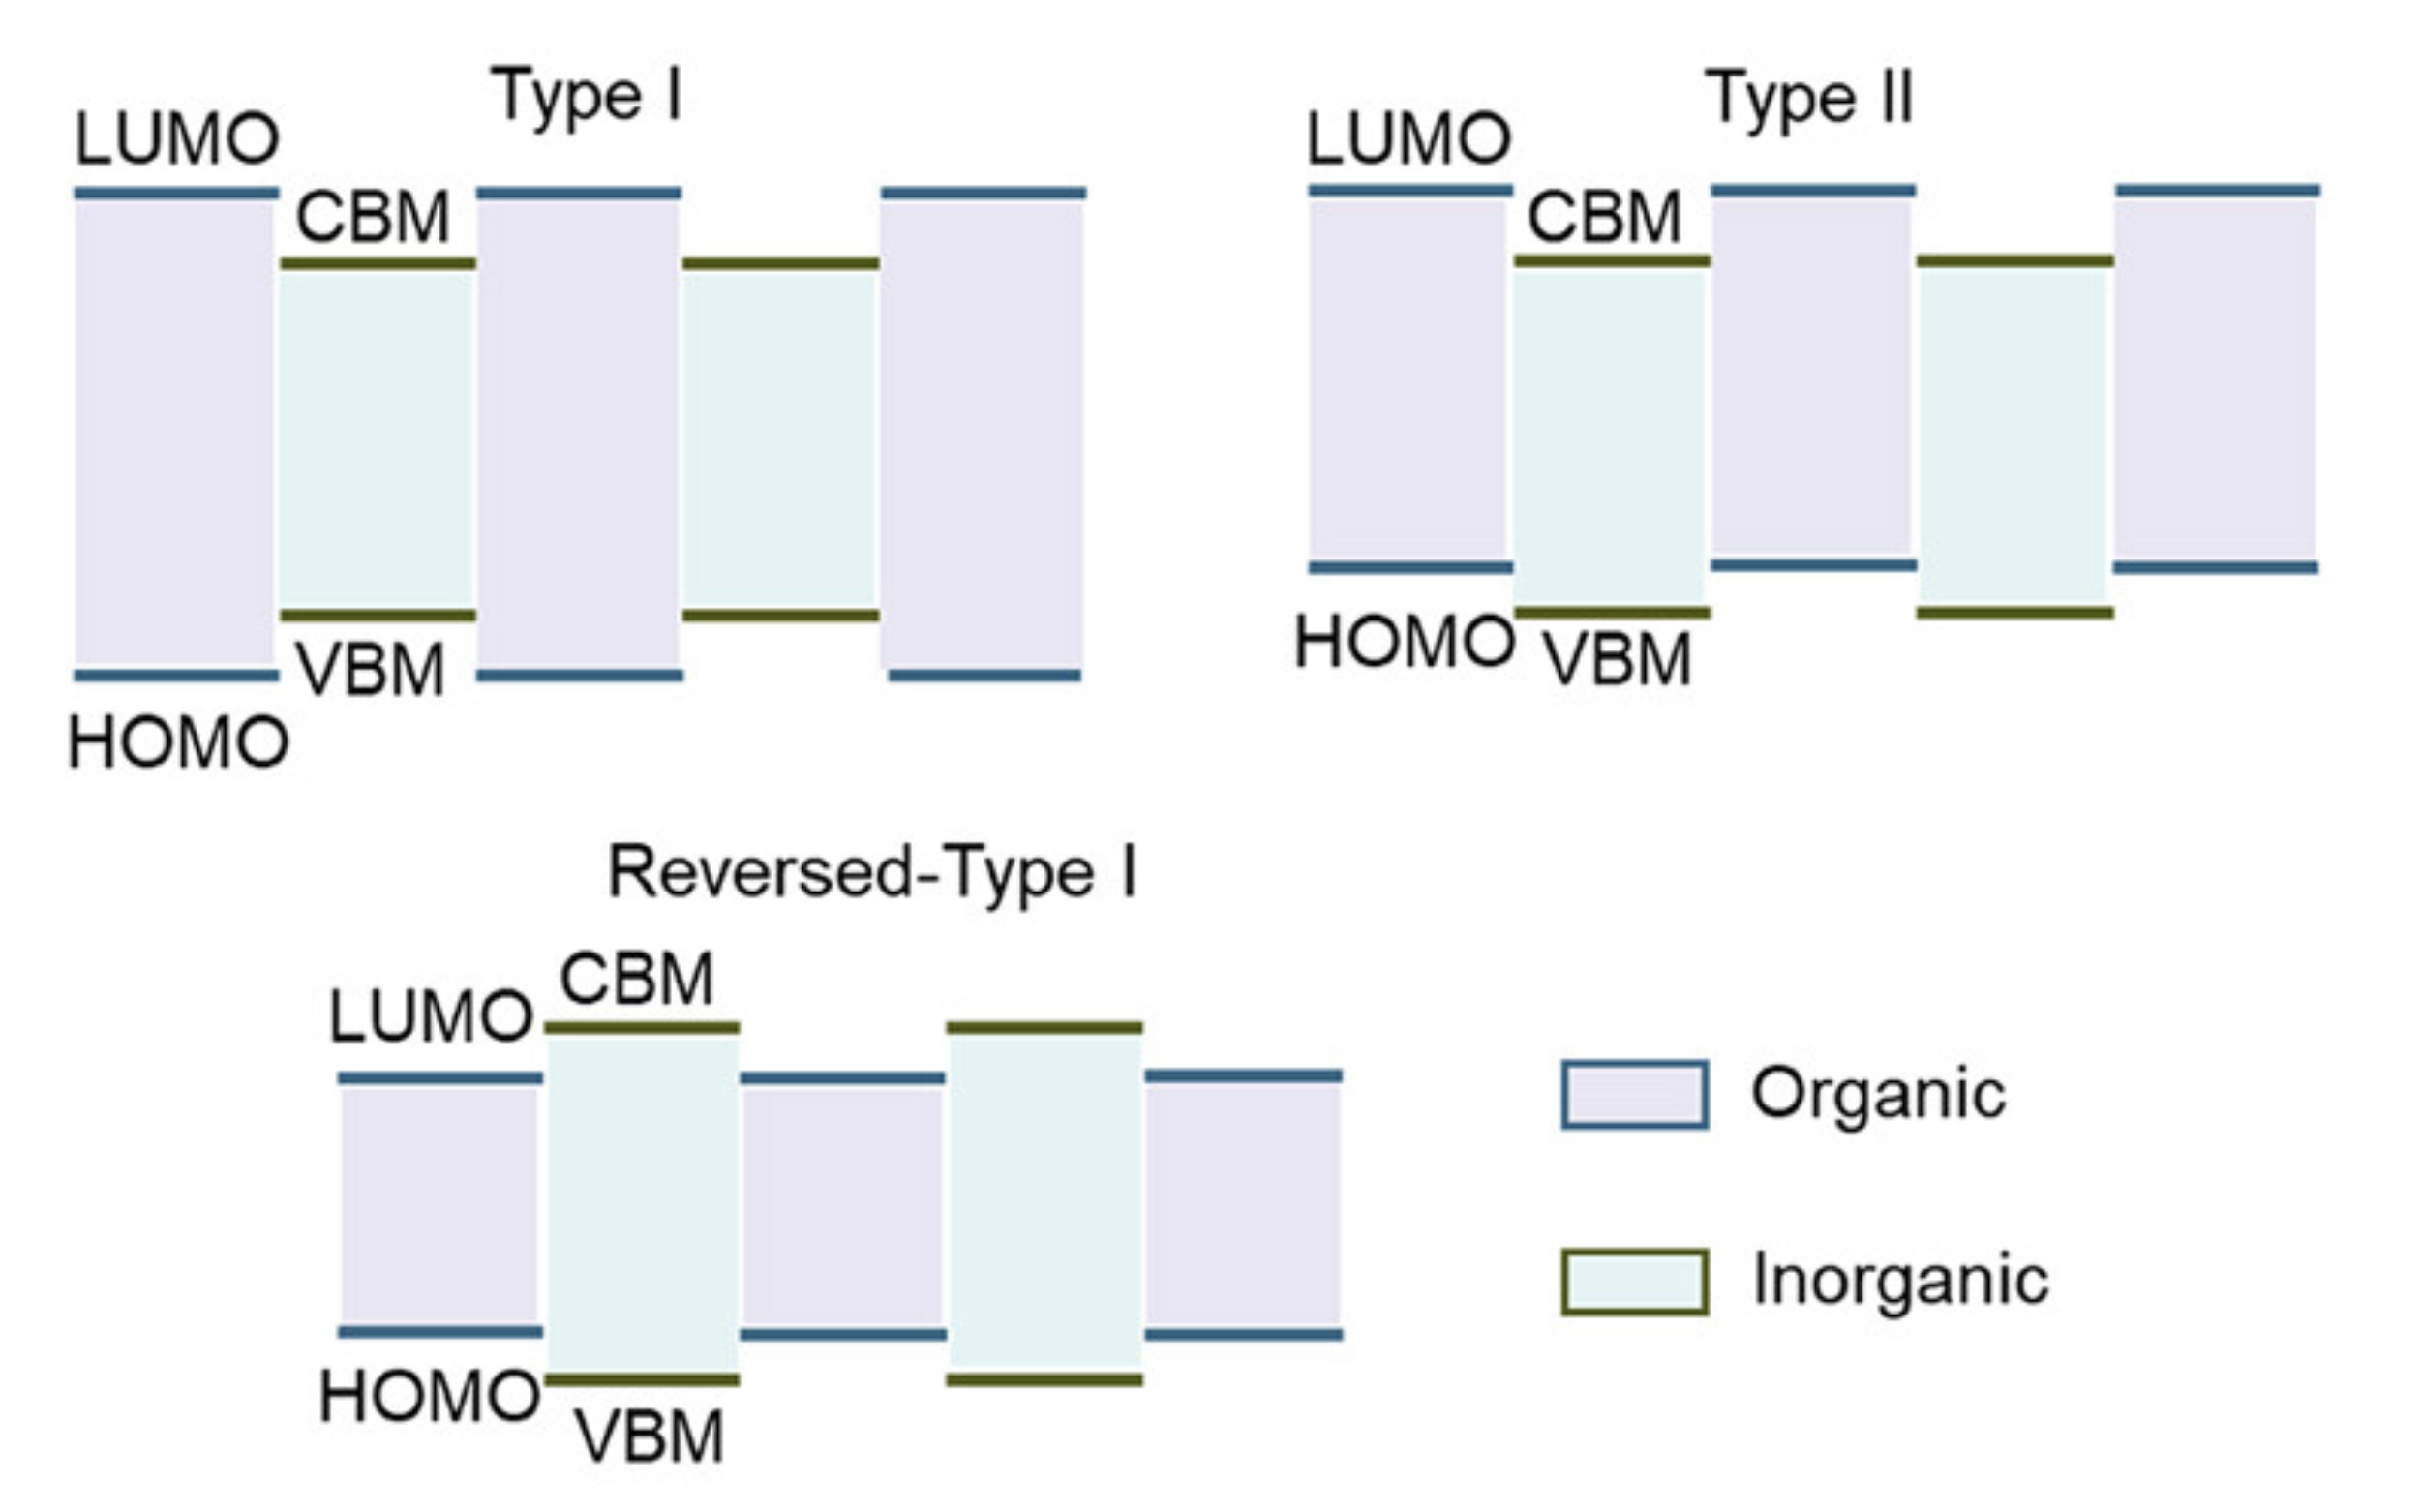
\includegraphics[width=0.9\textwidth]{figures/literature-review/figure2-12.png}
    \caption{Schematics of the quantum well effect in 2D perovskites\cite{RN304}.}
    \label{fig:figure2.12}
\end{figure}

One of the most actively explored strategies for improving 2D perovskite performance is tuning their quantum well structure through composition engineering. Energy-level alignments in these systems are generally categorized as type-I (straddling gap) or type-II (staggered gap), with four possible configurations. Most 2D perovskites naturally adopting a type-I configuration with organic component acts as the insulating barrier (Figure \ref{fig:figure2.12}). Research has explored various approaches to modulating energy level alignment, including altering the thickness and composition of the inorganic layer and tailoring the organic spacer design\cite{RN20,RN626,RN305}. Among these strategies, organic spacer engineering has emerged as the most promising, demonstrating the ability to achieve all four possible types of energy level alignment.

Despite these advancements, the tuning of energy level alignment remains limited, and many organic spacers have yet to be explored for further optimization. In the following section, we introduce design strategies for organic spacers to enhance their impact on perovskite properties.

\subsection{Design Strategies for Organic Spacers}

As mentioned above, the organic spacer cations in 2D perovskites play a pivotal role in determining their structural, electronic, and environmental stability properties. Rational design of these spacers enables the tuning of perovskite properties to optimize performance in optoelectronic devices.

The early discovery of organic spacers for 2D perovskites was largely serendipitous, driven by the limited availability of organic cations known to incorporate into the perovskite framework. Initial studies primarily focused on simple alkylammonium spacers, such as butylammonium (BA) and propylammonium (PA), with research efforts centred on varying spacer length or functional groups to improve film morphology and device performance\cite{RN135,RN504,RN217}. 

In recent years, spacer engineering has evolved significantly, shifting towards the deliberate design of organic cations with tailored functionalities. This includes the exploration of conjugated organic spacers, typically featuring aromatic systems such as benzene or thiophene rings\cite{RN218,RN31}. The introduction of conjugation has been shown to enhanced interactions between organic spacers, improved charge transport, and enable tunable optoelectronic properties\cite{RN228}. Additionally, spacer modification strategies now encompass functional group engineering—such as side-chain substitutions, fluorination, and positional adjustments of ammonium tethering groups—to finely control interlayer interactions, defect passivation, and environmental stability.

\begin{figure}[ht]
    \centering
    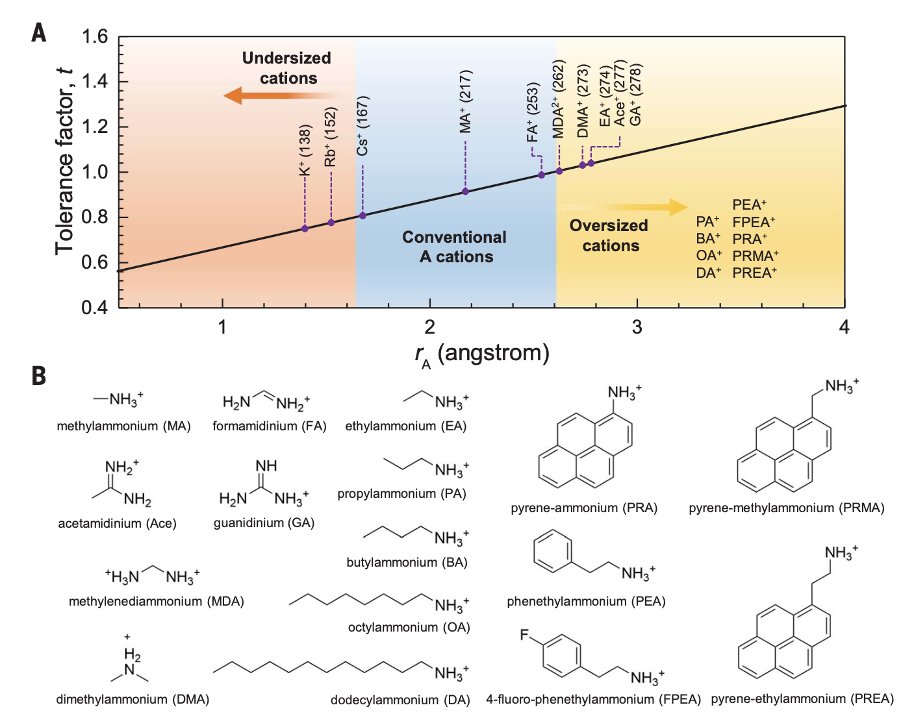
\includegraphics[width=\textwidth]{figures/literature-review/figure2-13.png}
    \caption{Molecular size constraints for organic spacers in 2D perovskites\cite{RN42}.}
    \label{fig:figure2.13}
\end{figure}

To maintain the perovskite framework, organic spacers must satisfy certain structural and chemical criteria. From a steric perspective, the size and shape of the organic spacer play a crucial role in determining whether it can fit within the inorganic framework and stabilize the 2D perovskite structure (Figure \ref{fig:figure2.13}). While there is no strict limitation on the length of the organic spacer—studies have successfully incorporated linear alkyl organic spacers with up to 18 carbon atoms into 2D perovskite framework\cite{RN637,RN638,RN639}—the cross-section area must remain within a certain threshold to avoid exceeding the available space within the 2D perovskite lattice\cite{RN519}. In particular, the cross-section width of the organic spacer, often approximated by the diameter of its conjugated backbone, should be smaller than width of the MX$_6$ octahedral unit\cite{RN20}. If the spacer is too bulky, studies have shown that it can lead to different structural dimensions or even disrupt the formation of a stable 2D lattice, leading to 0D or 1D perovskite\cite{RN640,RN641}.

Another critical consideration in designing organic spacers is the shape and configuration of the ammonium head group, which strongly influences hydrogen bonding. In 2D perovskites, this ammonium head typically fits into the cavity formed by the inorganic octahedral network, creating hydrogen bonds that stabilize the overall structure\cite{RN519,RN117}. The halide ions in the inorganic framework serve as hydrogen-bond acceptors, necessitating that the organic spacer contains a suitable hydrogen bond donor—typically an electron-deficient nitrogen bearing at least one hydrogen. Primary ammonium groups (i.e., $NH_3^+$) are widely used because they offer relatively strong hydrogen bonding, though secondary ($NH_2^+$) or tertiary ammonium group ($NH^+$) can also participate in hydrogen bond, albeit with generally lower bonding strength. Excessive steric hindrance around the nitrogen can impede its insertion into the inorganic pocket and weaken these critical bonds, potentially destabilizing the 2D perovskite. Typically, the hydrogen bond distance must remain below $\sim3.0-3.5 \AA$ to provide sufficient structural stabilization\cite{RN117}.

\begin{figure}[ht]
    \centering
    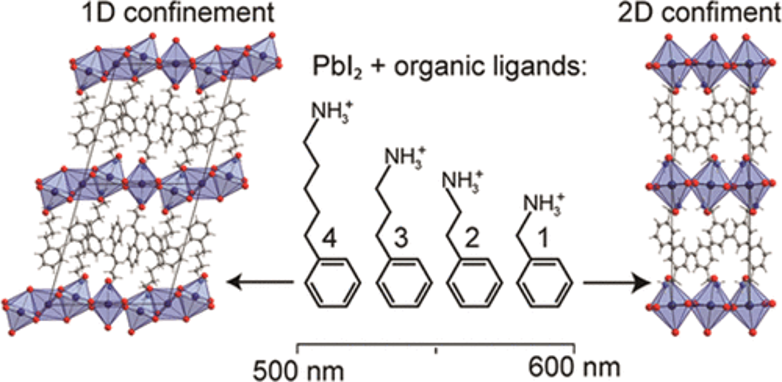
\includegraphics[width=0.9\textwidth]{figures/literature-review/figure2-14.png}
    \caption{Modulation of 2D perovskites formability by tuning linker length\cite{RN649}.}
    \label{fig:figure2.14}
\end{figure}

Recent work has demonstrated various strategies for modulating hydrogen bonding. In one study, researchers investigated organic spacers in which the ammonium tethering group was placed at different positions along the molecule, altering the distance between the ammonium head and the inorganic framework\cite{RN28}. The spacer with the weakest hydrogen bonding formed a one-dimensional (1D) perovskite, whereas the two stronger-bonding spacers yielded 2D structures. Another approach involved varying the length of linker segment between the ammonium head and the main body of the spacer, thereby increasing conformational flexibility and enhancing hydrogen-bond interactions with the inorganic lattice (Figure \ref{fig:figure2.14})\cite{RN86,RN649}. Additionally, functional group engineering—such as fluorination—has been shown to further strengthen hydrogen bonds, likely due to the high electronegativity and induced dipole moment of fluorine atoms\cite{RN211}.


Beyond the structural considerations necessary for forming a 2D perovskite, organic spacer engineering also provides opportunities to tailor electronic properties. In many cases, the organic spacer does not directly participate in the electronic structure of the inorganic framework, allowing it to act primarily as a structural template. For instance, shorter organic spacers can reduce the interlayer distance and thereby enhance out-of-plane charge transport\cite{RN179}. Additionally, adjustments to the inorganic octahedral tilting can further modulate the perovskite bandgap\cite{RN31}. Some conjugated organic cations—particularly those containing aromatic rings—are known to reduce energy barriers for charge transport relative to their alkyl-based counterparts\cite{RN239,RN88}.

\begin{figure}[ht]
    \centering
    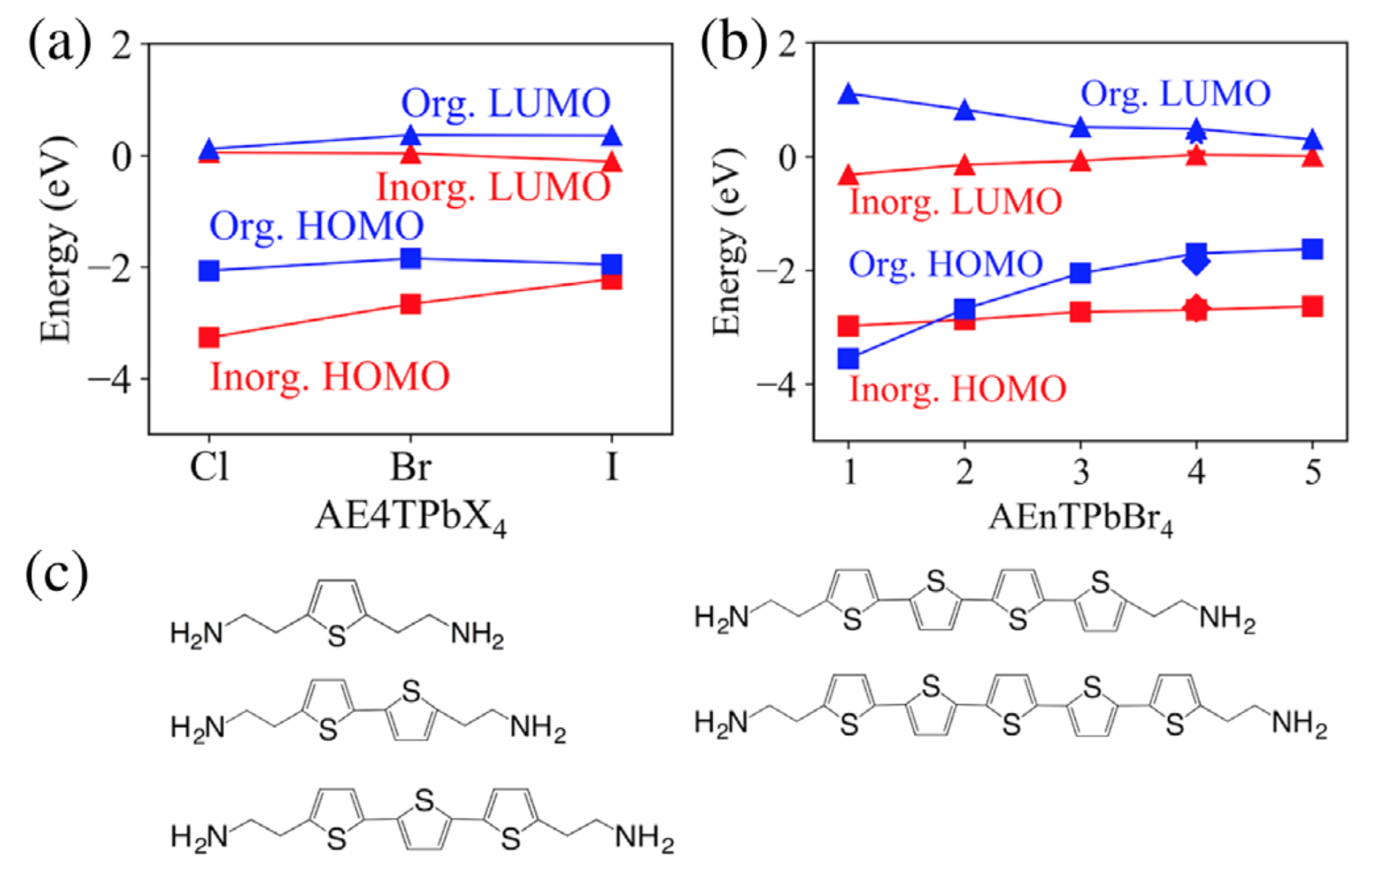
\includegraphics[width=\textwidth]{figures/literature-review/figure2-15.png}
    \caption{Engineering the energy level alignment in 2D perovskites by designing organic spacers\cite{RN18}.}
    \label{fig:figure2.15}
\end{figure}

Modifying the quantum well structure offers another route for electronic tuning. Introducing organic spacers with extended conjugation can shift the spacer’s frontier orbitals, potentially inverting the quantum-well alignment from type I to type II. Achieving this often requires complex spacer architectures with extended $\pi$-conjugation and functional-group modifications. In one study, organic cations featuring a $\pi$-conjugated pyrene backbone with varying linker lengths were introduced onto the perovskite surface. These cations contributed electronically to the surface band edges and influenced carrier dynamics, ultimately improving solar cell efficiency\cite{RN39}. In another series of studies (Figure \ref{fig:figure2.15}), oligothiophene-based organic spacers were incorporated into DJ-phase perovskites, with both DFT calculations and experimental results confirming that increasing the number of aromatic rings effectively tuned the energy-level alignment, leading to the realization of type-II alignment\cite{RN38,RN18}. Additionally, research on RP-phase perovskites has explored highly conjugated organic spacers, demonstrating that modifications to functional groups can achieve all four types of energy-level alignment. For instance, the introduction of electron-withdrawing units enabled type-II alignment, where the organic LUMO and inorganic VBM define the band edges. Meanwhile, incorporating a small bandgap unit facilitated a reversed type-I alignment\cite{RN20}. 

Despite the established design strategies for organic spacers in 2D perovskites, the optimization process remains highly complex. The intricate structural features of organic spacers, along with their interactions with the inorganic framework, introduce a vast number of variables that are challenging to fully understand through conventional trial-and-error methods or human intuition alone. To address this complexity, AI-driven approaches have emerged as powerful tools for accelerating material discovery and optimization. The following section explores recent advancements in AI-driven methodologies for 2D perovskites, with a particular emphasis on organic spacer design.

\subsection{AI-Driven Approaches for 2D perovskites}

ML methods have been extensively applied to the design of 3D perovskites, yet their use in guiding the discovery and optimization of 2D perovskites remains in a comparatively early stage. In 3D perovskites, a key focus has traditionally been an optimizing the inorganic frameworks—often represented by elemental compositions that are relatively straightforward for computational methods to handle\cite{RN314,RN422,RN317}. By contrast, 2D perovskites incorporate both inorganic layers and organic spacers. The design challenge therefore shifts prominently to selecting and engineering the organic spacer, which must meet specific geometric (e.g., size constraints) and chemical (e.g., functional group compatibility) requirements.

Given that ML-assisted discovery of 2D perovskites is still in its early stages, relevant studies in this field remain scarce. Therefore, to provide a broader perspective, below we review ML application in three closely related research areas: organic spacer design in 2D perovskites, hybrid materials interface design, and organic materials design. 

\begin{figure}[ht]
    \centering
    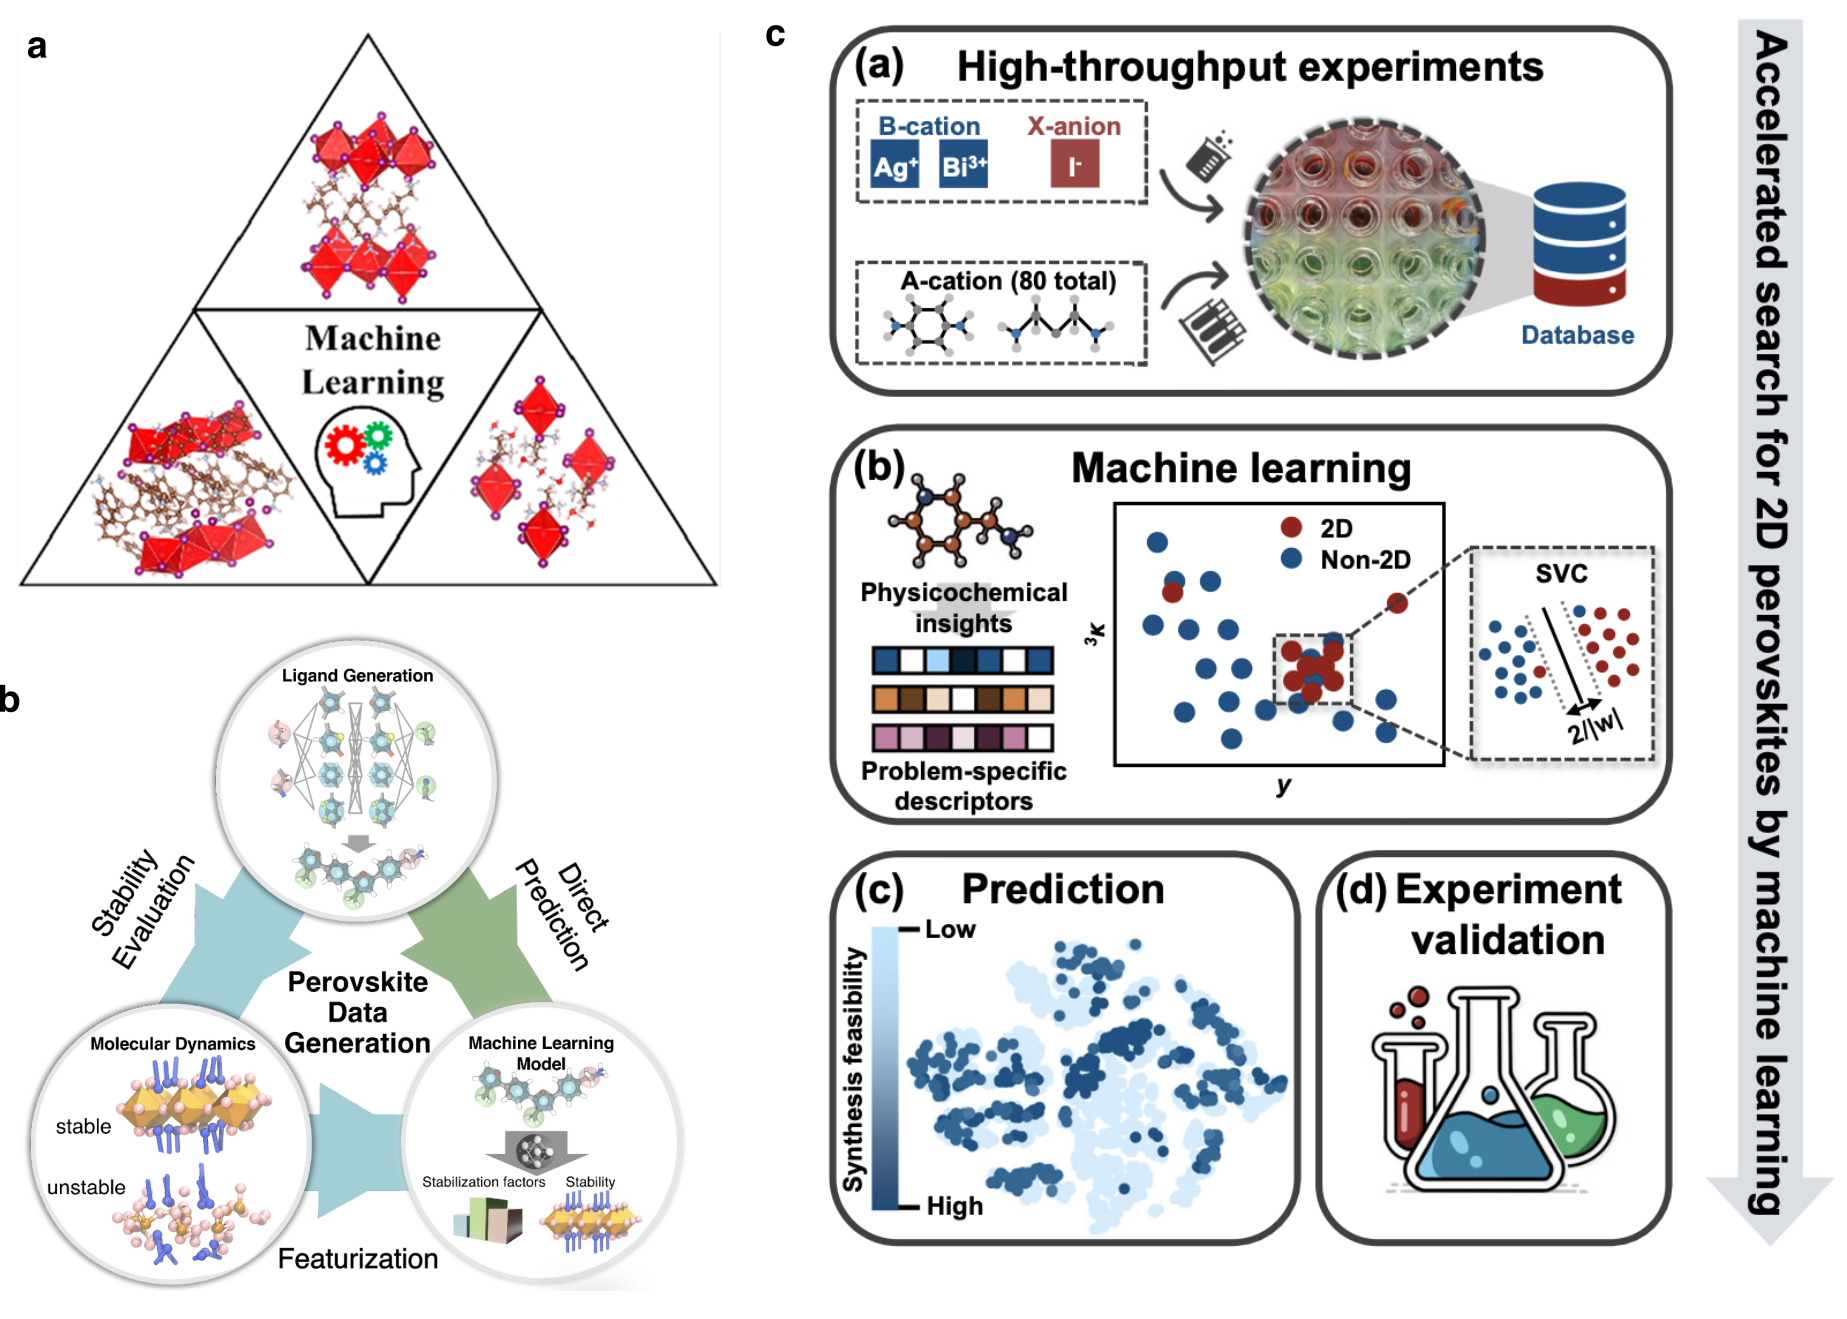
\includegraphics[width=\textwidth]{figures/literature-review/figure2-16.png}
    \caption{Machine learning workflows for 2D perovskite design\cite{RN283,RN12, RN315}.}
    \label{fig:figure2.16}
\end{figure}

The virtually unbounded chemical space of possible organic spacers has driven researchers to explore ML and other data-driven strategies for 2D perovskites (Figure \ref{fig:figure2.16}). An early study has used ML models trained on 86 reported organic spacers in lead-based 2D perovskites to derive design rules for predicting the perovskite dimensionality of five new organic spacers\cite{RN12}. Recent approaches have expanded the scope of spacer exploration considerably. For instance, Wu et al. utilized a ML model trained on 80 high throughput synthesized lead-free double perovskites to evaluate the synthesis feasibility of 8,460 organic spacers from PubChem\cite{RN315}. In another study, molecular dynamics simulations on over ten-thousand hypothetical organic spacers were used as training data to select six new ligands for perovskite synthesis\cite{RN283}. 


Beyond 2D perovskites, similar ML workflows have been applied to other hybrid materials interfaces involving small molecules, particularly in passivation materials for perovskite solar cells\cite{RN13,RN538,RN630}. In these studies, ML workflows typically follow a three-step approach. First, the physiochemical descriptors are selected based on domain knowledge. Second, the descriptors are computed from the organic molecule structure. Finally, these descriptors are used as input features for supervised machine learning models to predict key properties. For example, a recent study used various regression models to predict the power conversion efficiency (PCE) of perovskite solar cells passivated by ammonium salts, using a set of physiochemical descriptors\cite{RN538}. 

Compared to hybrid perovskites, ML-assisted design of organic materials is a relatively mature field, with well-established methods for molecular representation and advanced machine learning models\cite{RN612,RN563,RN610,RN564}. The most critical aspect of ML workflows in organic materials is how molecules are represented. Common molecular representations include: 

(1) SMILES (Simplified Molecular Input Line Entry System) – An invertible molecular representation widely used in text-based ML models. 

(2) Molecular fingerprints – Such as Morgan fingerprints or Extended Connectivity Fingerprints (ECFPs), which have been extensively applied to polymer design, peptide engineering, and organic emitter discovery. 

For instance, a recent study used a 2048-bit Morgan fingerprint to represent heat-resistant polymers, combined with a feed-forward neural network to down-select promising candidates from a virtual library\cite{RN610}. These representation techniques, combined with advanced ML models, have proven effective for guiding molecular design. However, directly applying these techniques to 2D perovskites is not straightforward due to the added complexity of the organic–inorganic interface.

A major limitation of the current ML approaches in 2D perovskites is their reliance on forward design workflows, which require exhaustive brute-force screening of chemical space. Since organic spacers must be predefined before descriptors can be calculated, the approach is not invertible, preventing direct generation of new molecular structures from target properties. Moreover, descriptor-based representations often fail to fully capture the molecular complexity of organic spacers. Such brute-force screening can be computationally expensive and may miss promising regions of chemical space if the initial library is not sufficiently diverse. Therefore, inverse design—where desired properties are defined a priori, and algorithms propose candidate molecules or structures—holds the promise of accelerating materials discovery for 2D perovskites. 

Furthermore, much of the pioneering ML work on 2D perovskites has been centred on questions of formability and stability, a critical gap remains in the application of AI-assisted workflow to predict physical properties of 2D perovskites. Energy level alignment, a key property controlling the spatial distribution and transfer of charge carriers and excitations in semiconducting materials and their interfaces, directly impacts the performance of optoelectronic devices. Different from well-studied elemental and compound semiconductors, organic and inorganic components in hybrid perovskites are heterogeneous with separate energetics, forming quantum-well-like structures\cite{RN18}. Although 2D perovskites have been investigated using traditional workflows, such as the Edisonian approach\cite{RN20} and high-throughput calculations\cite{RN236,RN617}, systematic exploration of the energy level alignment through AI-assisted approaches is still in its early stages\cite{RN618}, presenting a significant opportunity for advancement. 

\section{Summary and Research Gaps}\label{section:section2-3}

In the preceding sections, we introduced the two main pillars of this thesis: AI-assisted materials discovery—with particular attention to inverse design methodologies—and the design challenges posed by 2D perovskites, especially in the context of organic spacers. Their intersection is the central focus of this work.

From the perspective of 2D perovskite design, the vast chemical space of organic spacers necessitates the use of data-driven and machine learning techniques. These materials exhibit highly intricate structure–property relationships, with many potentially relevant features that are difficult to fully grasp through traditional approaches. To tackle this complexity, we focus on DJ-phase n=1 Pb–I-based perovskites as a prototype system for studying structure–property relationships. Insights gained from this prototype can then be generalized to other 2D perovskite phases and alternative inorganic frameworks. We choose energy level alignment as our target property, as it is crucial for optoelectronic applications yet remains insufficiently understood.

From the viewpoint of AI-assisted inverse materials design, this 2D perovskite system presents an equally compelling challenge. Unlike more extensively studied materials with large, well-curated datasets, 2D perovskites are relatively data-scarce and uniquely hybrid in nature, requiring careful consideration of both organic and inorganic components. While inverse design methodologies have shown promise for inorganic materials, organic molecules, and polymers, 2D perovskites introduce additional constraints—such as spacer size limitations and the complex organic–inorganic interface—that necessitate novel AI-driven approaches.

Moreover, the insights gained from this research could extend beyond 2D perovskites to a broader class of hybrid materials, where the intricate interplay between organic and inorganic components defines material properties. As emerging materials fields often suffer from data scarcity, developing machine learning strategies tailored to these challenges is essential. By leveraging AI in such contexts, we aim to contribute to a generalizable framework for hybrid material discovery, enabling data-driven innovation in materials science.

This thesis addresses several critical research gaps in the field of AI-driven 2D perovskite design:

\begin{itemize}
    \item Lack of large, high-quality datasets for 2D perovskites – Unlike well-established materials, 2D perovskites suffer from data scarcity. Existing datasets are often small, inconsistent, or lack standardization, limiting the ability of machine learning models to generalize effectively.
    \item Limited understanding of structure–property relationships – A quantitative and predictive understanding of how organic spacer chemistry influences electronic properties and synthesizability remains underdeveloped. The complexity of organic–inorganic interactions make it challenging to establish clear design rules.
    \item Challenges in inverse design for 2D perovskites – Existing inverse design models do not fully accommodate the unique constraints of hybrid materials, such as the size limitations of organic spacers and the chemical constraints associated with functional group compatibility.
    \item Challenges in AI-assisted approaches for hybrid materials – The absence of a standardized ML workflow for hybrid materials poses a significant barrier. Feature selection remains underdeveloped, and machine learning models struggle to encode key chemical and structural descriptors necessary for accurately modelling organic–inorganic interactions.
\end{itemize}

Addressing these challenges requires robust, AI-driven frameworks tailored to 2D perovskite design—particularly those that incorporate domain expertise, and feature property-driven design. The present thesis aims to bridge some of these gaps by exploring inverse design workflows that couple molecular design with inorganic framework constraints, ultimately accelerating the discovery of high-performance 2D perovskite materials.

    \chapter[Methodology]{Methodology} \label{c:method} 

This chapter outlines the methodology developed for the inverse design of DJ-phase 2D perovskites. Section \ref{section:section3-1} provides an overview of the overall design framework, which integrates chemical space establishment, property prediction, and synthesis feasibility. Section \ref{section:section3-2} introduces the core component of the workflow: an invertible and interpretable molecular fingerprint tailored for organic spacer design. The subsequent sections detail the key pipelines of the framework, including high-throughput calculations (Section \ref{section:section3-3}), machine learning model development and evaluation (Section \ref{section:section3-4}), and the two-step synthesis feasibility screening process (Section \ref{section:section3-5}).


\section{Overview of the inverse design workflow}\label{section:section3-1}

\begin{figure}[ht]
    \centering
    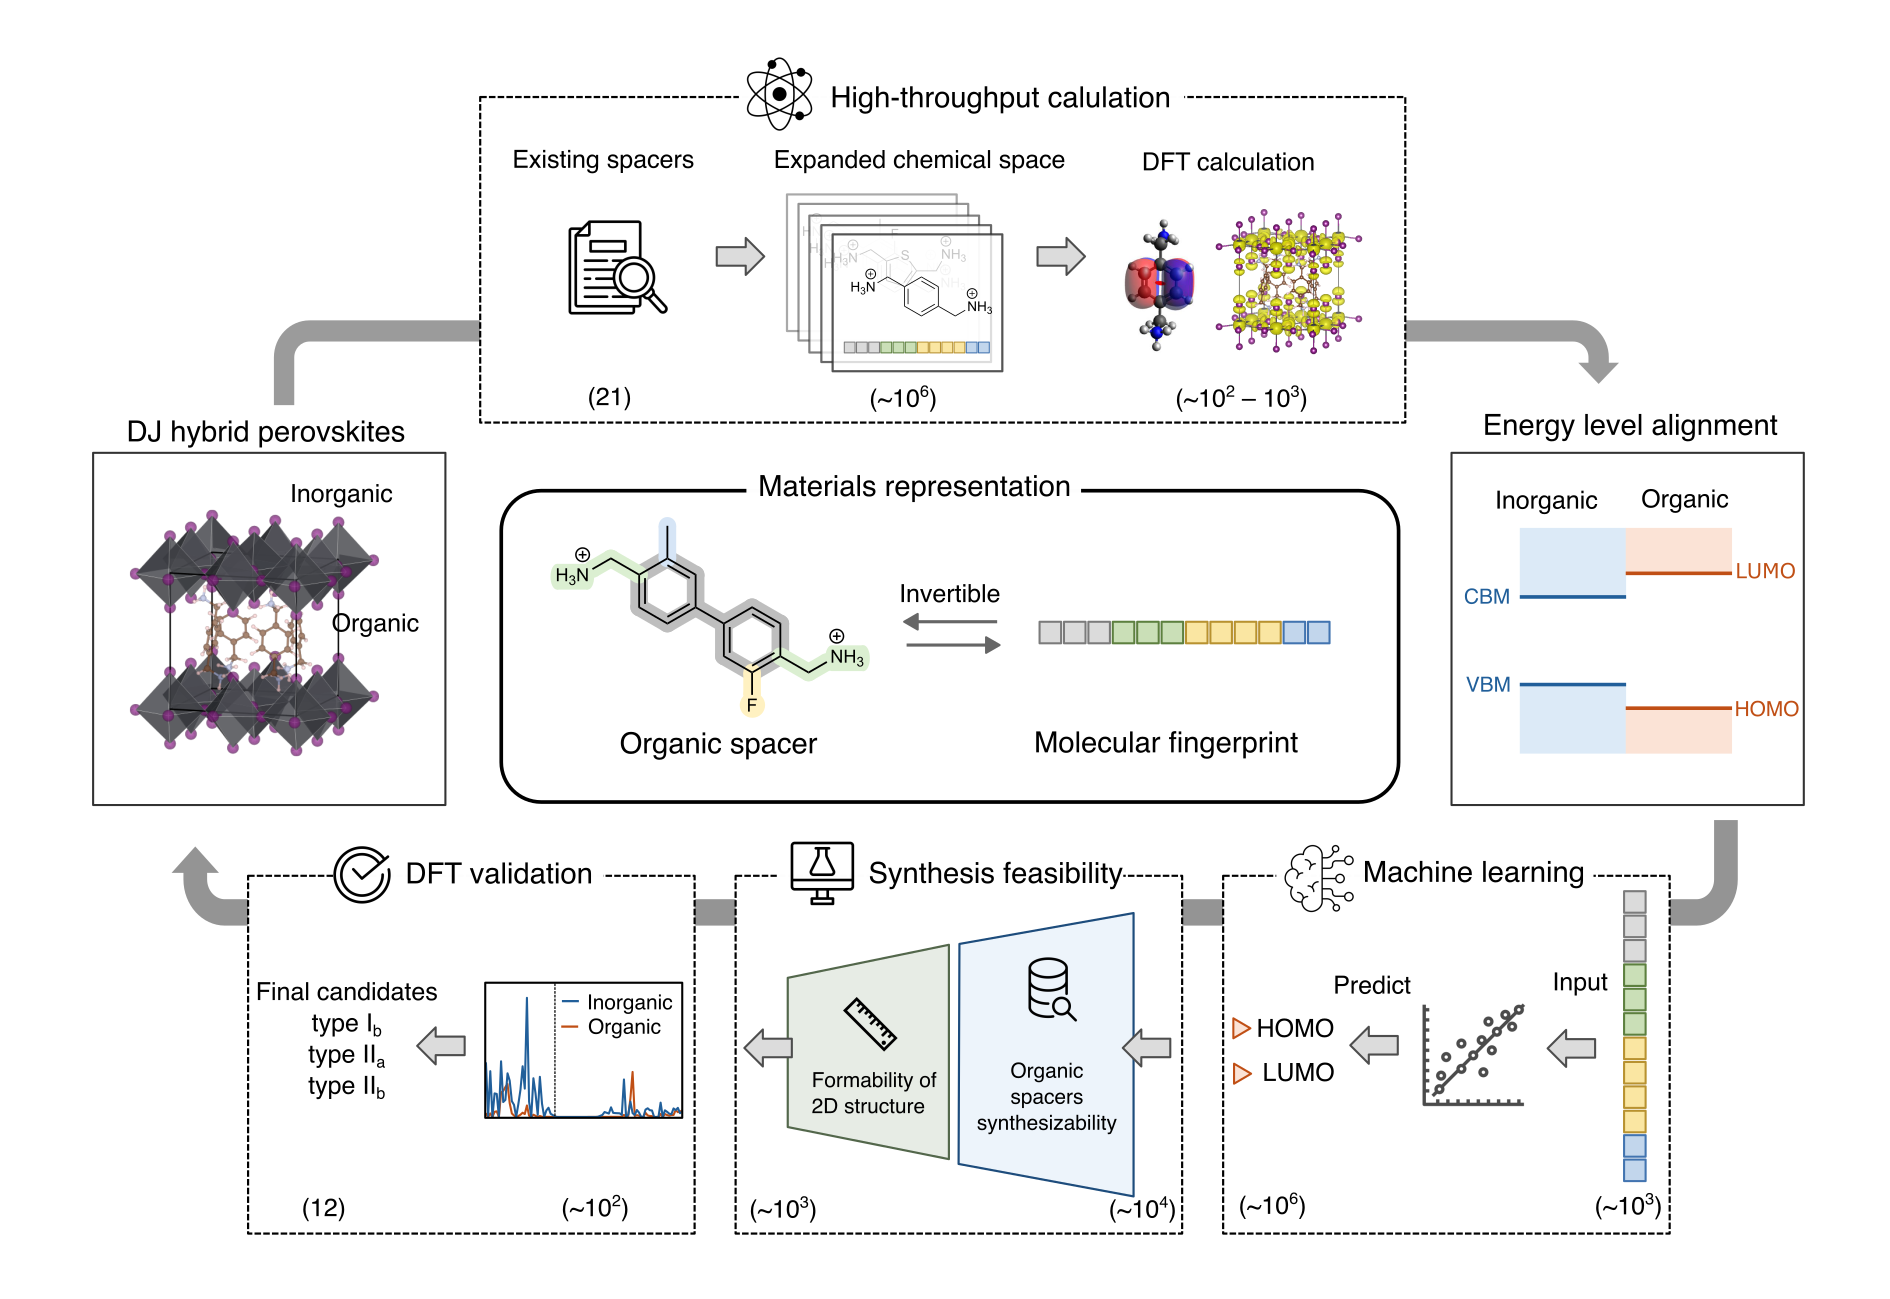
\includegraphics[width=\textwidth]{figures/methodology/figure3-1.png}
    \caption{AI-assisted inverse design workflow for discovering DJ perovskites with targeted energetics and synthesis feasibility. }
    \label{fig:figure3.1}
\end{figure}

The AI-assisted inverse design workflow is illustrated in Figure \ref{fig:figure3.1}. This workflow hinges on a unique 12-digit fingerprint representation scheme to navigate the chemical space of organic spacers, integrating DFT calculations, machine learning, and synthesis feasibility screening. First, hypothetical candidates are generated using a molecular morphing approach and selected for DFT calculation. Second, the DFT data are used to train interpretable machine learning models, accelerating property predictions and revealing structure-property relationships. Third, synthesis feasibility is assessed based on the synthetic accessibility of organic spacers and their potential to form stable 2D structures. Finally, these 2D perovskites undergo DFT validation to confirm their energy level alignment, leading to a selection of recommended candidates.

This workflow was designed based on the unique nature of 2D hybrid perovskites and the targeted property of band alignment. It begins with chemical space expansion using a molecular morphing approach. To realize an invertible representation of conjugated diammonium organic spacers, they are encoded into a compact 12-digit fingerprint vector. Based on the physical insights obtained on 21 existing spacers reported for DJ perovskites, we generated the fingerprints of approximately $4\times10^6$ hypothetical spacers with complexity comparable to the reported ones. High-throughput density functional theory (DFT) calculations were then used to evaluate the energy levels of the corresponding hybrid perovskites within a designated subset of the chemical space, which were used as the training data. Next, various regression models were trained using fingerprints as input features and organic frontier levels as target property, aiming to extract insights on the structure-property relationship. The hypothetical spacers were then down selected using a two-step synthesis feasibility screening funnel based on their availability in the PubChem database and multiple reported formability descriptors specific to forming 2D perovskite structures. Lastly, feasible candidates for targeted energy level alignment types are validated using DFT calculation. By integrating these components, the workflow facilitates inverse design of DJ perovskites with rarely explored Ib, IIa and IIb band alignment types. 

\begin{figure}[htbp]
    \centering
    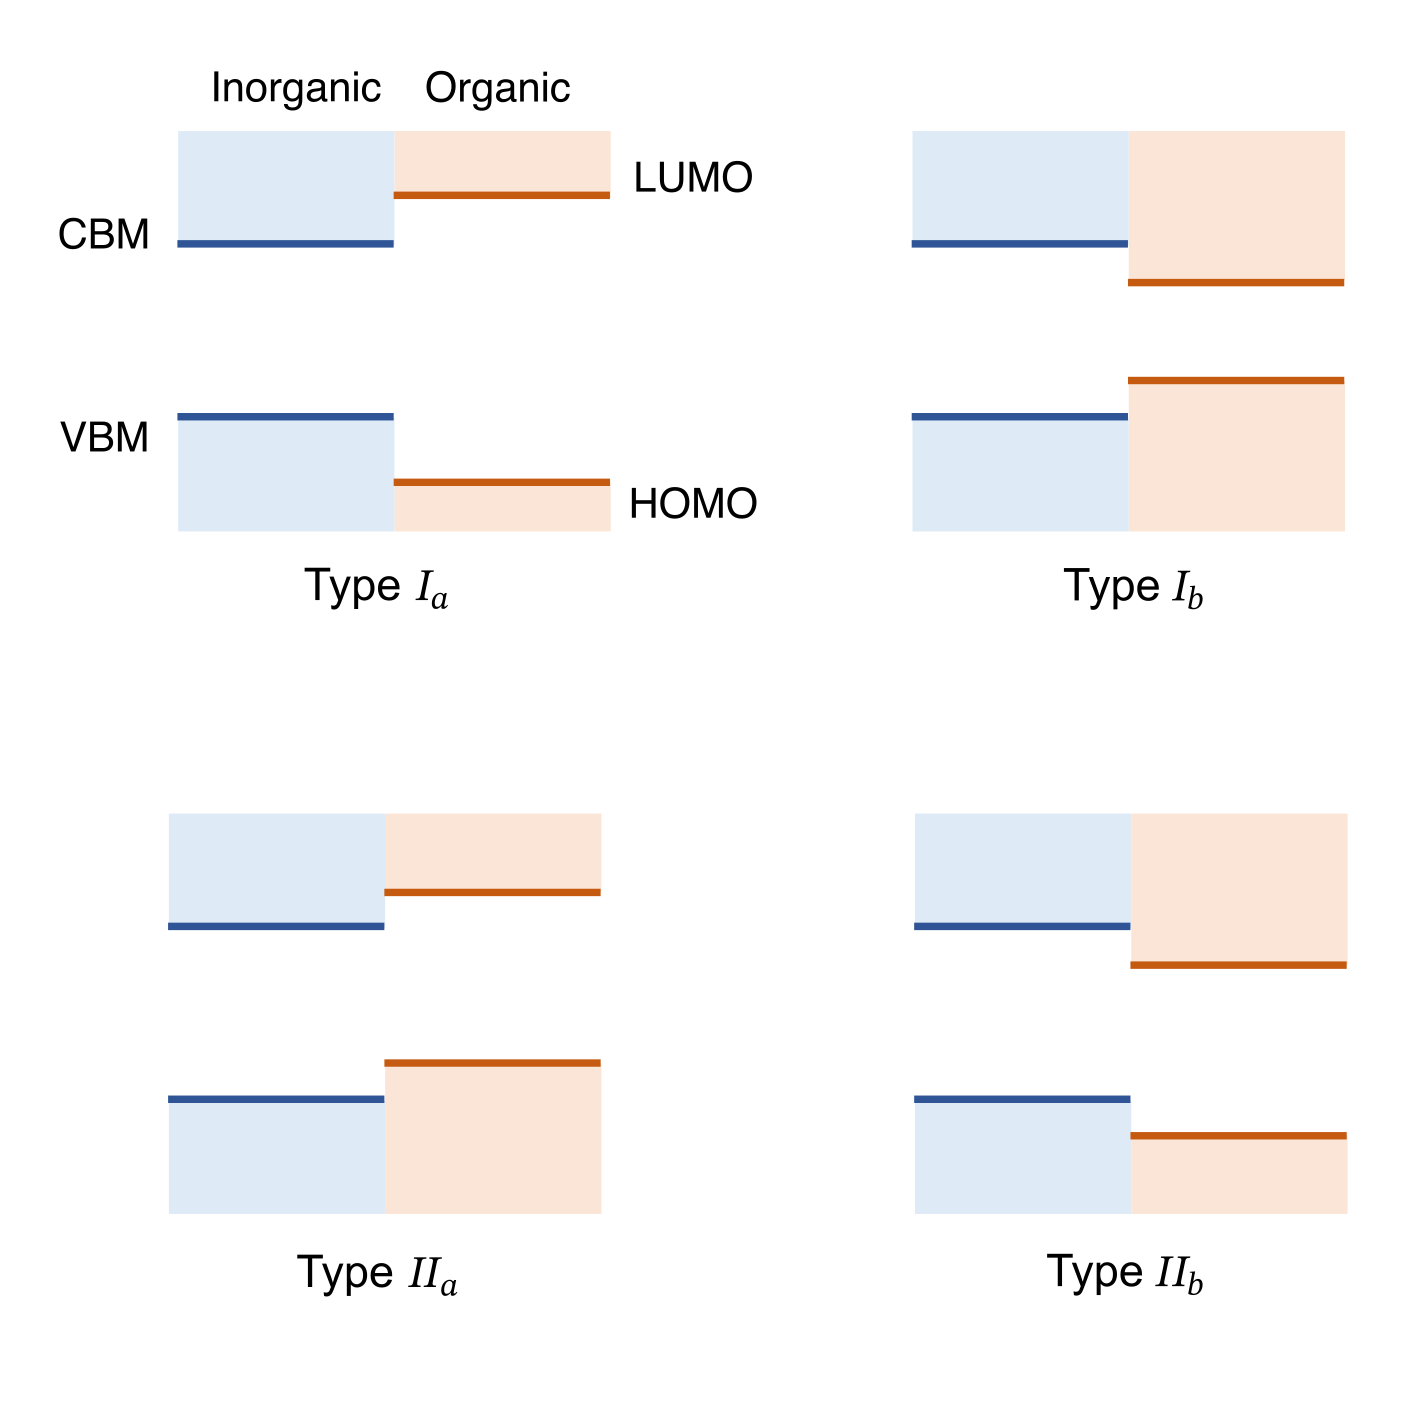
\includegraphics[width=0.6\textwidth]{figures/methodology/figure3-2.png}
    \caption{Schematic representation of energy level alignment types in 2D perovskites. }
    \label{fig:figure3.2}
\end{figure}

The classification of the energy level alignment types is shown in Figure \ref{fig:figure3.2}. In type I alignment, both low-energy electrons and holes are localized in the same component: type Ia in the inorganic layers and type Ib in the organic layers. In type II alignments, electrons and holes are separated between different components: in type IIa, electrons are localized in the inorganic layers and holes in the organic layers, whereas in type IIb, the reverse occurs. It should be noted that the designations “a” and “b” are sometimes interchanged in the literature depending on the component being emphasized\cite{RN18}. In other studies, only type I and type II are referenced without further categorization\cite{RN20}, and type Ib in our context is occasionally described as “reversed type I”\cite{RN606}. Notably, alignment type Ia is referred to as type Ib in some literature\cite{RN104,RN18}; here, we defined type Ia as the configuration where inorganic states serving as the band edges.

While the components of this workflow—database generation, high-throughput calculations, machine learning, and DFT validation—are common to AI-assisted materials discovery\cite{RN321,RN553}, the distinctive feature here is the integration of an invertible materials representation. Invertibility is a key attribute for materials representations in inverse design\cite{RN361}, ensuring two-way conversion between molecular structure and their representation. This type of invertible representation has been applied to some materials systems\cite{RN412,RN354}, but this is the first implementation in the context of hybrid materials. The absence of a versatile scheme of organic spacer representation has confined 2D perovskite research to forward design approaches, limiting the exploration of available chemical space. As we will show in this thesis, the workflow developed herein overcomes these limitations, facilitating the energy level alignment prediction. In addition, we expect that this fingerprint-based workflow will be generalized to investigate the correlation of other material properties with organic motifs in a wide range of hybrid material systems. 

\section{Invertible Molecular Fingerprints}\label{section:section3-2}

\begin{figure}[ht]
    \centering
    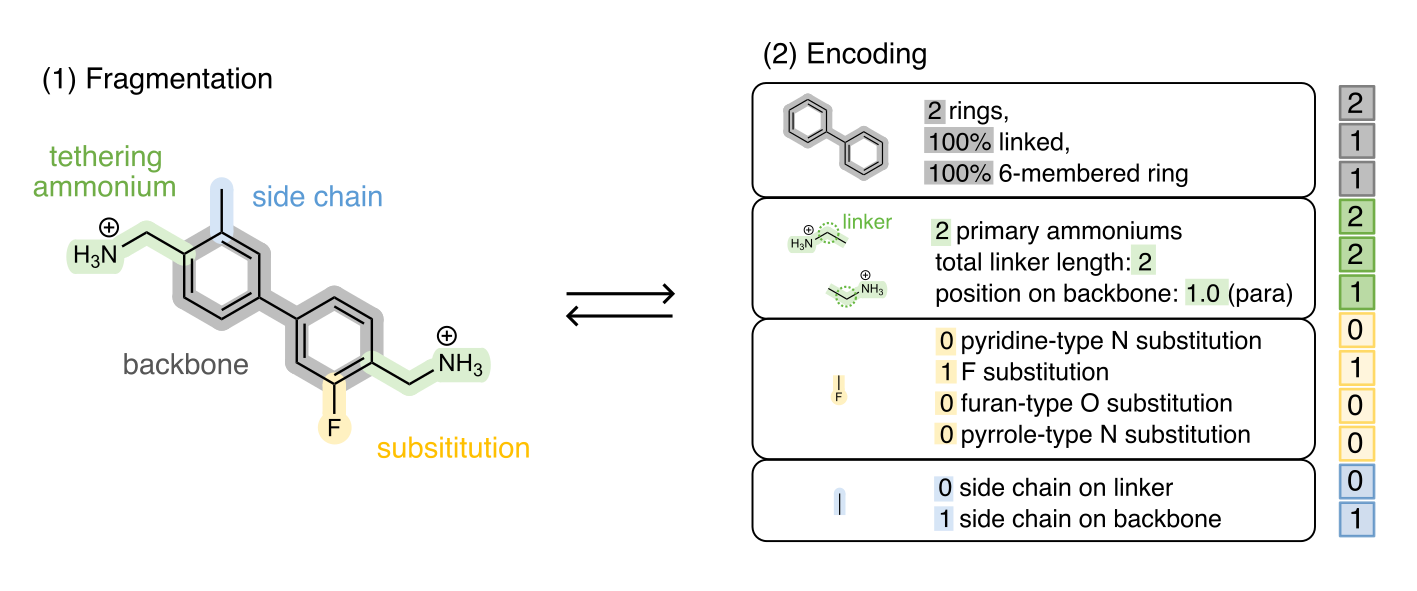
\includegraphics[width=\textwidth]{figures/methodology/figure3-3.png}
    \caption{Invertible molecular fingerprint representation for organic spacers in DJ perovskites.}
    \label{fig:figure3.3}
\end{figure}

Figure \ref{fig:figure3.3} depicts an overview of our fingerprinting scheme, which is based on the specific attributes of conjugated organic cations in 2D DJ perovskites, comprising two key components: molecular fragmentation and functional group encoding. Organic spacers are first fragmented into their building blocks (backbone, tethering ammonium, side chain, and substitutions) and then these building blocks are further encoded into a 12-digit fingerprint. 

\textbf{Fragmentation}

\begin{figure}[htbp]
    \centering
    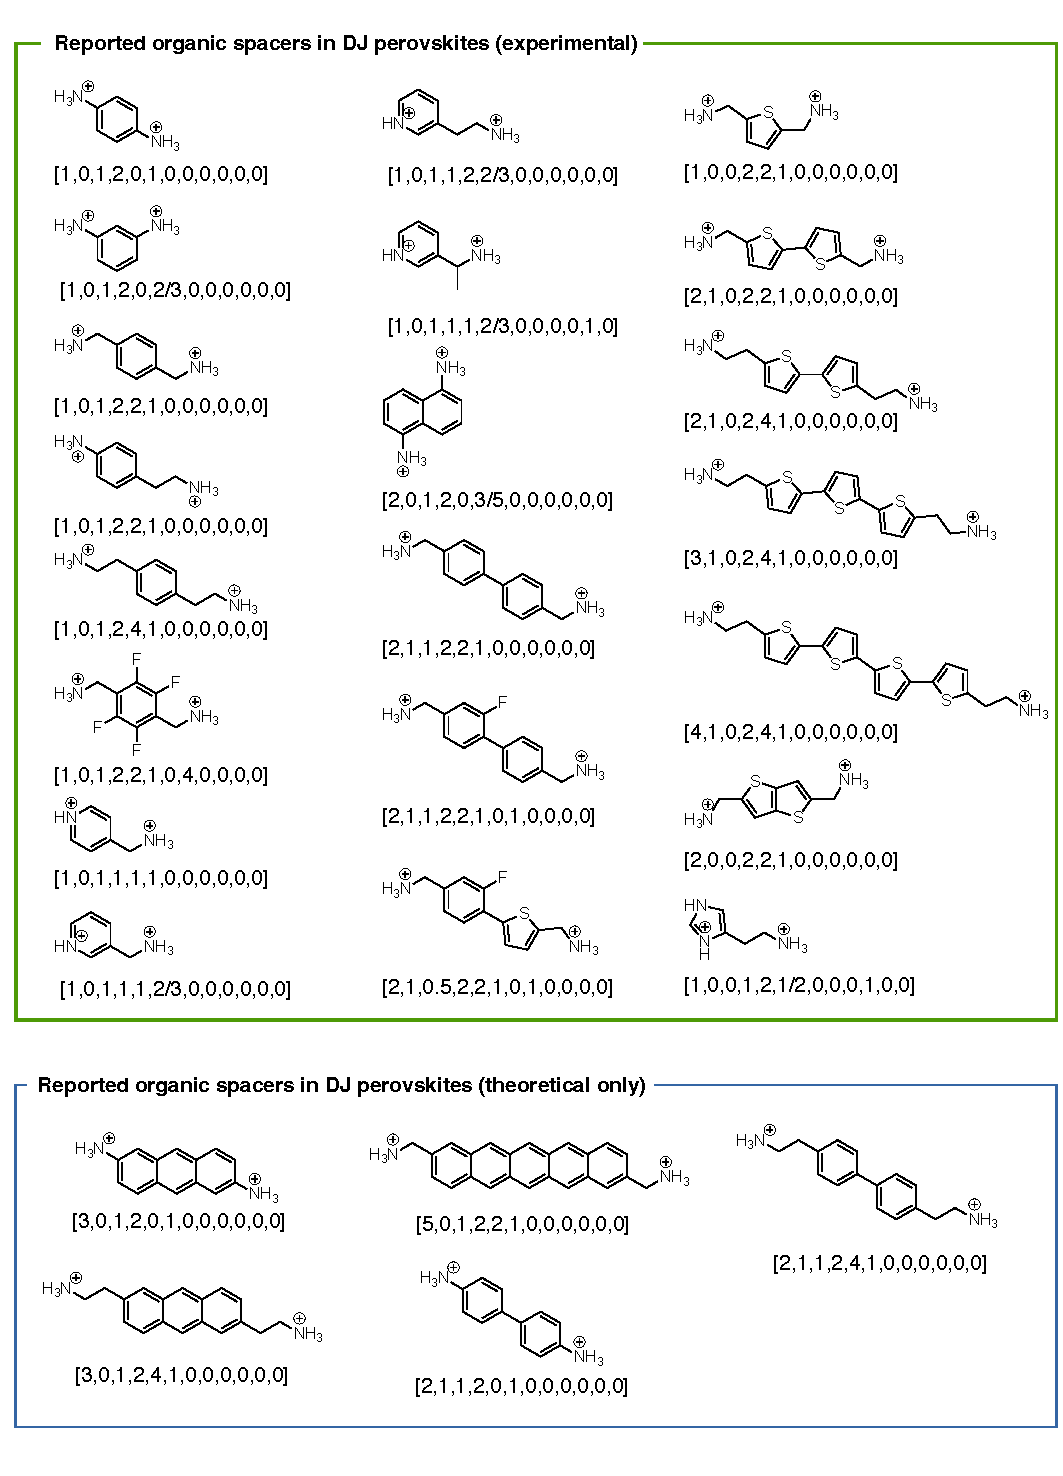
\includegraphics[width=\textwidth]{figures/methodology/figure3-4.pdf}
    \caption{Reported organic spacers included in this study with their molecular fingerprint.}
    \label{fig:figure3.4}
\end{figure}

\begin{figure}[htbp]
    \centering
    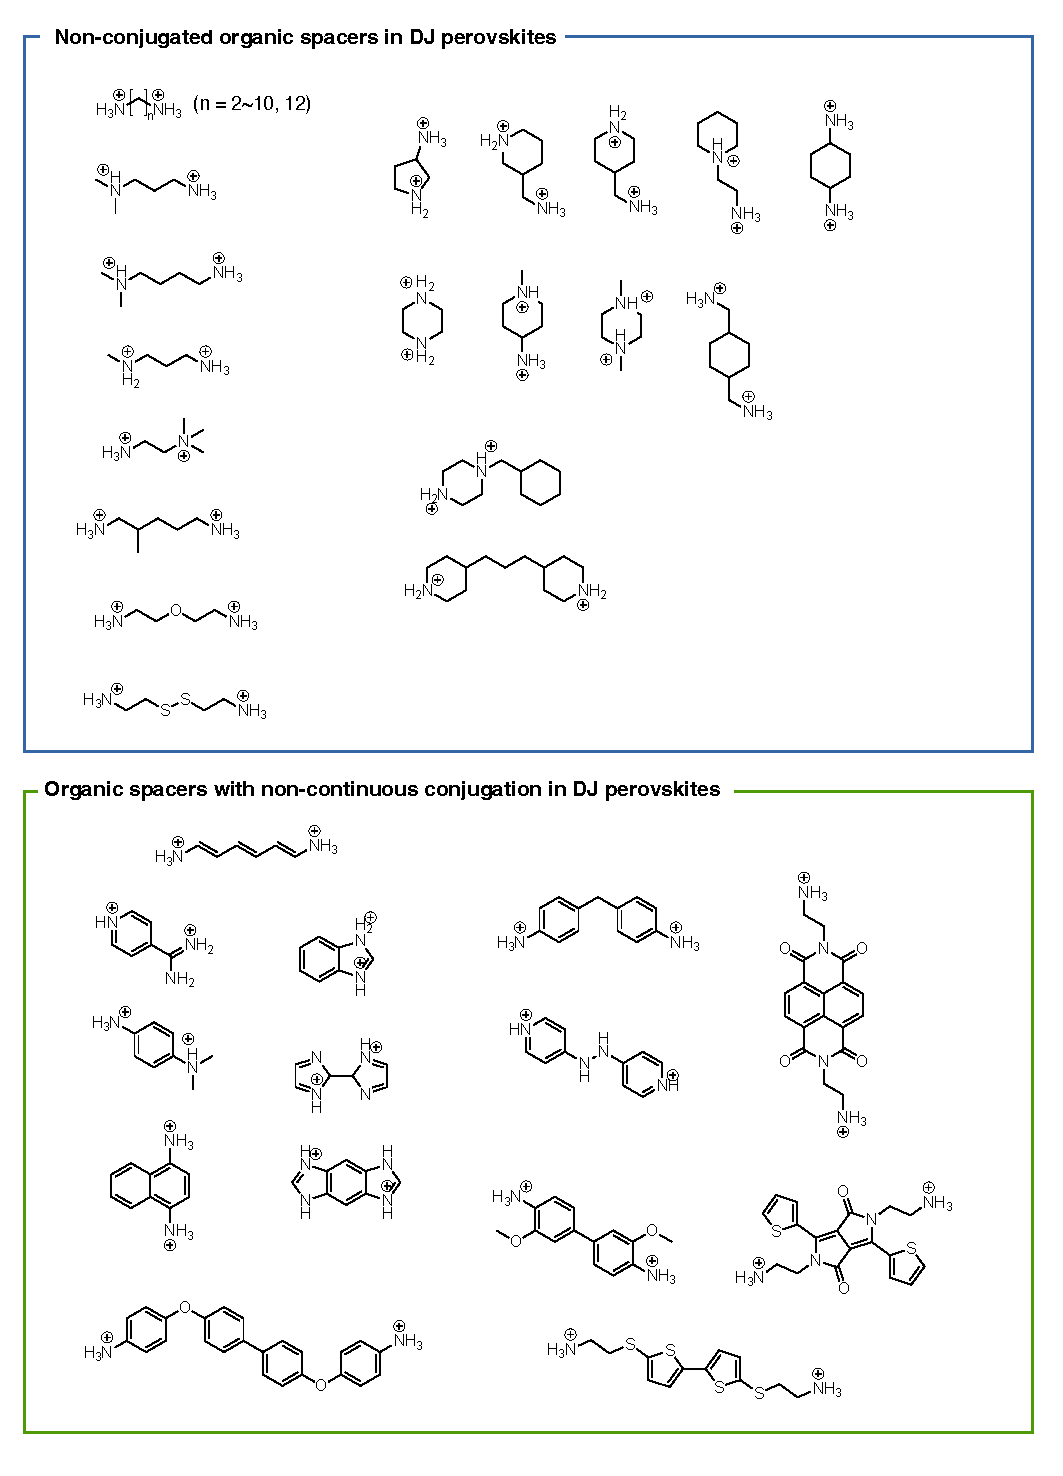
\includegraphics[width=\textwidth]{figures/methodology/figure3-5.pdf}
    \caption{Organic spacers excluded from the scope of this study.}
    \label{fig:figure3.5}
\end{figure}

The fragmentation is designed considering the structural motifs shared by reported conjugated diammonium spacers, as shown in Figure \ref{fig:figure3.4}. The DJ-phase organic spacers explored in this work are assumed to consist of four fragments: 

(1) a conjugated backbone of aromatic rings; 

(2) two tethering ammonium groups that anchor the spacer to the inorganic framework; 

(3) optional heteroatom substitutions;

(4) optional side chains. 

In this work, we limit the heteroatom substitutions to fluorine (F), oxygen (O), and nitrogen (N) on aromatic rings (benzene and thiophene). This simplification is based on two primary considerations: (1) their widespread use in semiconducting organic spacers within 2D perovskite systems, and (2) the need to preserve a chemically interpretable and synthetically accessible design space. Although including additional heteroatoms such as chlorine (Cl), bromine (Br), or phosphorus (P) could enhance electronic diversity, doing so would substantially expand the chemical space, increase fingerprint complexity, and introduce greater uncertainty in terms of synthetic feasibility and structural compatibility with the perovskite lattice.

These structural constraints significantly narrow the chemical space from a potentially immense size (estimated at $\sim10^{60}$ molecules for small organic molecules, as recognized in the context of drug discovery\cite{RN458}) to a much smaller subspace of organic spacers. 

We should note that the resulting chemical space is not exhaustive, leaving out some spacers, for example ones with alkyl backbones or non-continuous conjugation (Figure \ref{fig:figure3.5}). This fingerprinting scheme leads to a chemically relevant and computationally manageable set of organic cations (vide infra), giving rise to 2D DJ perovskite candidates with tailored properties. We primarily focused on semiconducting $\pi$-conjugated molecules due to their high relevance to optoelectronic applications of 2D perovskites and rich chemical diversity.

\textbf{Encoding}

\begin{figure}[ht]
    \centering
    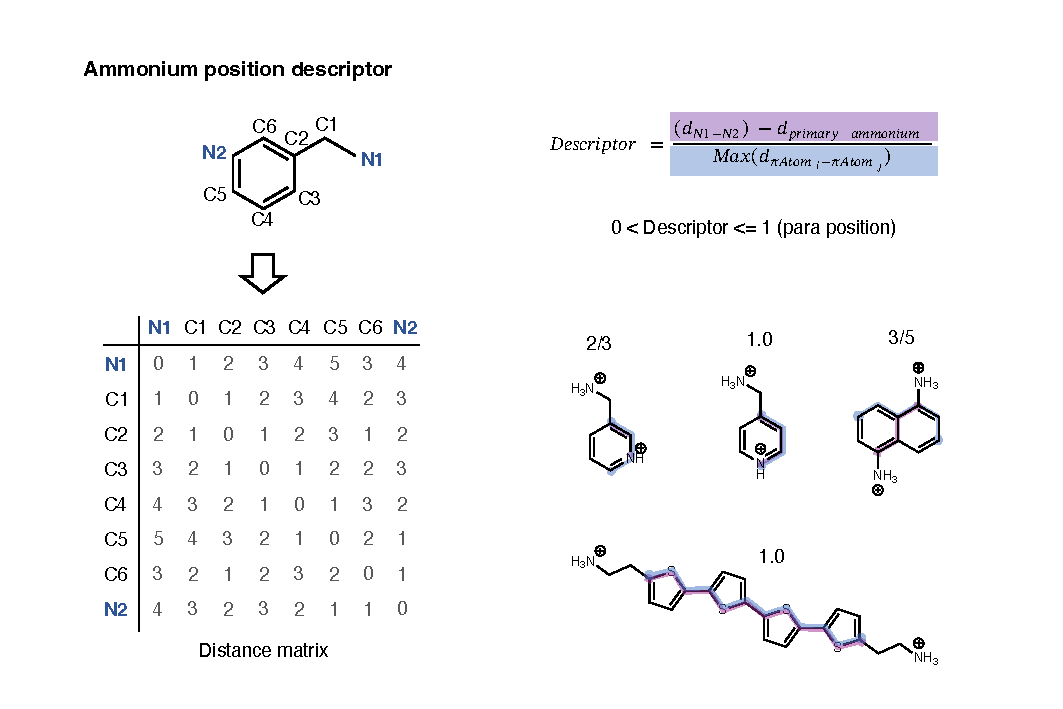
\includegraphics[width=\textwidth]{figures/methodology/figure3-6.pdf}
    \caption{Illustration of the ammonium position descriptor.}
    \label{fig:figure3.6}
\end{figure}

The encoding component of the scheme translates molecular structure into a fingerprint vector containing 12 customized descriptors, each representing a specific structural feature. Eleven descriptors are obtained by counting functional groups, while a unique “ammonium position” descriptor is derived from a distance matrix (Figure \ref{fig:figure3.6}). The main principle is to choose a minimal number of descriptors to reduce computational cost while these descriptors must be sufficient to describe the organic spacers relevant to DJ perovskites. As we will show later in the ML results in Chapter \ref{c:result-1}, there is minimal overlap between the descriptors, and they capture essential features for energy level prediction. 

For high-throughput purposes, all organic spacer structures in this study were stored in the Simplified Molecular Input Line Entry System (SMILES) format, a widely used textual representation of molecular structure. Molecular fingerprinting was performed to extract key structural and chemical descriptors automatically using the RDKit library in Python. The workflow took the SMILES representation of the organic spacer as input and returned a set of 12 organic descriptors, categorized as follows:

\begin{enumerate}
    \item Conjugated backbone descriptors: number of rings; percentage of ring linkages; percentage of six-membered rings
    \item Tethering ammonium descriptors: number of primary ammonium groups ($NH_3^+$); linker length (distance between ammonium groups and backbone); and ammonium position on the backbone
    \item Heteroatom substitution descriptors: number of nitrogen atoms (pyridine-type); number of fluorine atoms, number of oxygen atoms (furan-type); number of nitrogen atoms (pyrrole-type)
    \item Side chain descriptors: number of side chain attached to linkers; number of side chains attached to the backbone 
    
\end{enumerate}

Descriptors were computed using SMARTS (SMiles ARbitrary Target Specification) patterns, enabling the identification and counting of specific functional groups. A new descriptor, the ammonium position on the backbone, was developed specifically for this work. This descriptor quantifies the relative position of tethering ammonium groups on the conjugated backbone using a distance matrix approach, as depicted in Figure \ref{fig:figure3.6}.

The ammonium position descriptor is derived from the molecular skeleton using a distance matrix. This descriptor is calculated as the ratio of the maximum distance along the conjugated backbone to the distance between the tethering ammonium group and the backbone. Representative organic spacers with their corresponding ammonium position descriptors are shown in Figure \ref{fig:figure3.6}.

We should note that the molecule-fingerprint correspondence is not exclusive, in other words, some molecular isomers share the same fingerprint. Although additional descriptors, or longer fingerprints (e.g., heteroatom substitution position, and side chain position) could offer more structural detail, we found such features have minimal impact on electronic properties, making the current fingerprinting scheme sufficient for predicting new DJ perovskites with all four band alignment types.

\begin{figure}[ht]
    \centering
    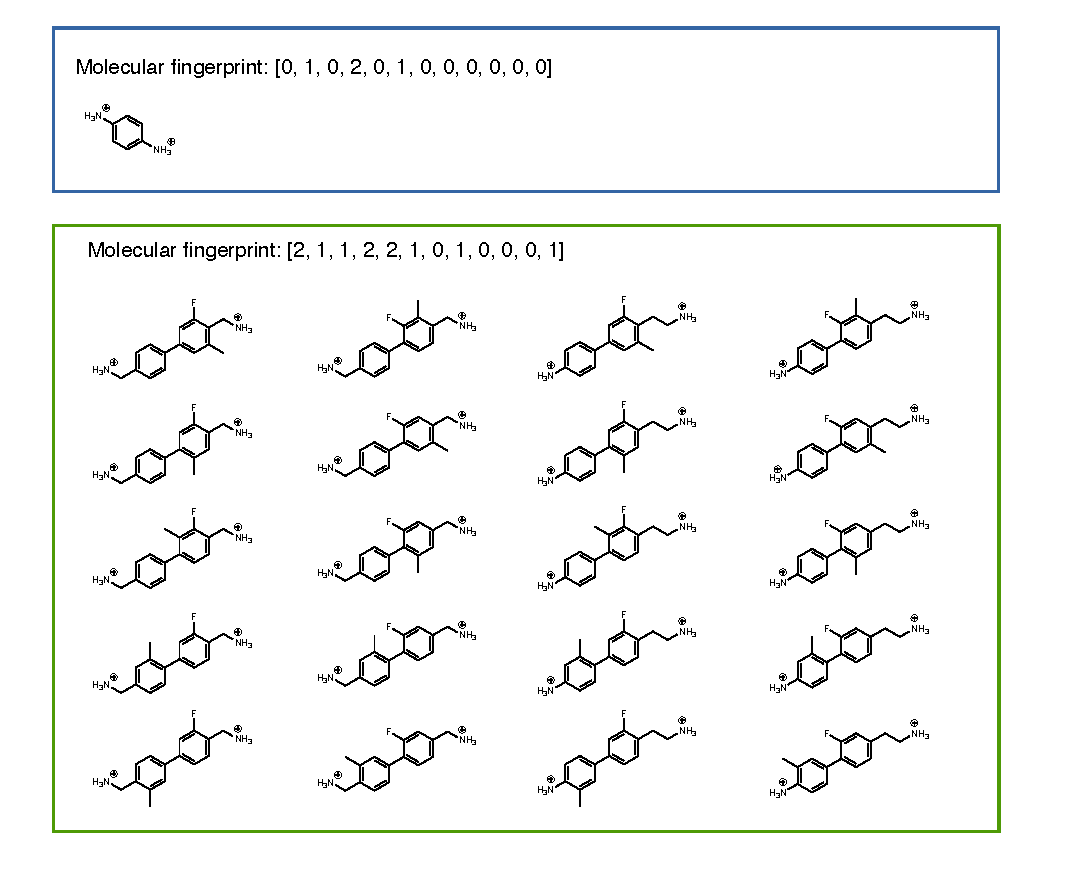
\includegraphics[width=\textwidth]{figures/methodology/figure3-7.pdf}
    \caption{An illustration of one-to-one (top) and one-to-multiple (bottom) mappings between a molecular fingerprint and its corresponding organic spacer(s).}
    \label{fig:figure3.7}
\end{figure}

Figure \ref{fig:figure3.7} illustrates the relationship between a fingerprint and its corresponding organic spacer(s). The upper panel shows a one-to-one mapping, where a fingerprint corresponds to a single organic spacer. In contrast, the lower panel shows a one-to-many mapping, where multiple organic spacers (isomers) share the same fingerprint, including the example shown in Figure \ref{fig:figure3.3}. These isomers may differ in structural features such as the position of heteroatom substitution, side chain placement, or the linker length between tethering ammonium groups. While such variations may affect to a certain extent the chemical and physical properties of the cations, the the energy levels are almost the same due to the shared molecular backbone. However, these isomers may have different levels of synthesis feasibility, which warrants elucidation based on future detailed analysis and experimental efforts. At this stage, no additional screening is applied to these isomers. All molecules corresponding to a given fingerprint are retained in the dataset to preserve the full chemical diversity for downstream analysis.

In previous AI-assisted 2D perovskite discovery efforts, organic spacers are typically represented using physiochemical descriptors\cite{RN315,RN283}, but an effective molecular representation scheme that can explicitly capture the molecular structure has not been established. In the myriad research fields involving organic molecules, the structural variations are often encoded using digits (e.g., fingerprints), strings (e.g., SMILES), or graph-based methods\cite{RN361}. Among these, fingerprinting methods—such as the widely adopted but non-invertible 2048-digit Morgan fingerprint—have demonstrated their efficiency in AI-assisted workflow\cite{RN610,RN549}. In contrast, our 12-digit fingerprint scheme has been tailored according to the specific attributes of 2D hybrid perovskites, offering several advantages. First, it is efficient, with minimal redundancy and overlap between descriptors, ensuring a compact representation that captures structural variation most relevant to DJ perovskites. Second, it is interpretable, enabling human experts to extract meaningful insights into the encoded structural variations. Finally, it is invertible, allowing direct mapping back to the molecular structure by both human experts and machines, which is essential for inverse design.

\section{High-throughput calculation}\label{section:section3-3}

\textbf{Molecular morphing}

Molecular morphing was implemented as a systematic method to explore chemical space by generating variants of molecular structure. The process used reaction SMARTS patterns implemented in the RDKit library to iteratively apply predefined chemical transformations. This approach performs stepwise modifications on a starting molecular structure, generating new variants while adhering to defined chemical constraints. 

\begin{figure}[ht]
    \centering
    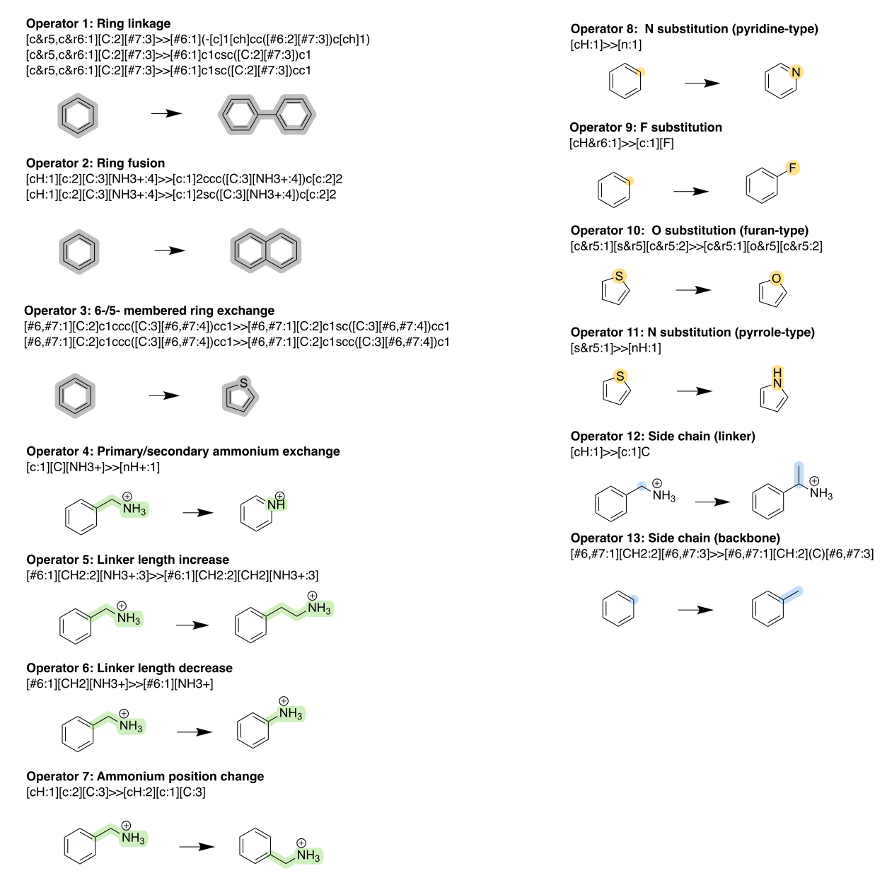
\includegraphics[width=0.9\textwidth]{figures/methodology/figure3-9.png}
    \caption{List of molecular morphing operators used in this study for generation of hypothetical organic spacers.}
    \label{fig:figure3.8}
\end{figure}

The molecular morphing process began with  PDMA, a well-characterized prototype molecule, represented in SMILES format. As shown in Figure \ref{fig:figure3.8}, a set of 13 morphing operators, encoded as 17 unique SMARTS patterns, was defined to ensure that each transformation adhered to established chemical constraints. These morphing operation include:
increasing number of rings, substituting heteroatoms on aromatic rings, modifying linker lengths, etc.

Each operator was applied iteratively to the starting molecule to generate new molecular structures. The newly generated molecules were stored as SMILES strings, ensuring compatibility with downstream fingerprinting and modelling workflows.

PDMA was chosen as the starting molecule due to its structural simplicity and extensive study in the literature. Figure \ref{fig:figure3.9} illustrates the distribution of existing spacers across generations when different candidates are selected as $G_0$ molecules. PDMA (top right) was selected because it results in most existing spacers appearing in early generations, demonstrating its structural simplicity and suitability for easy transformation into other molecular structures via morphing operations.


\begin{figure}[ht]
    \centering
    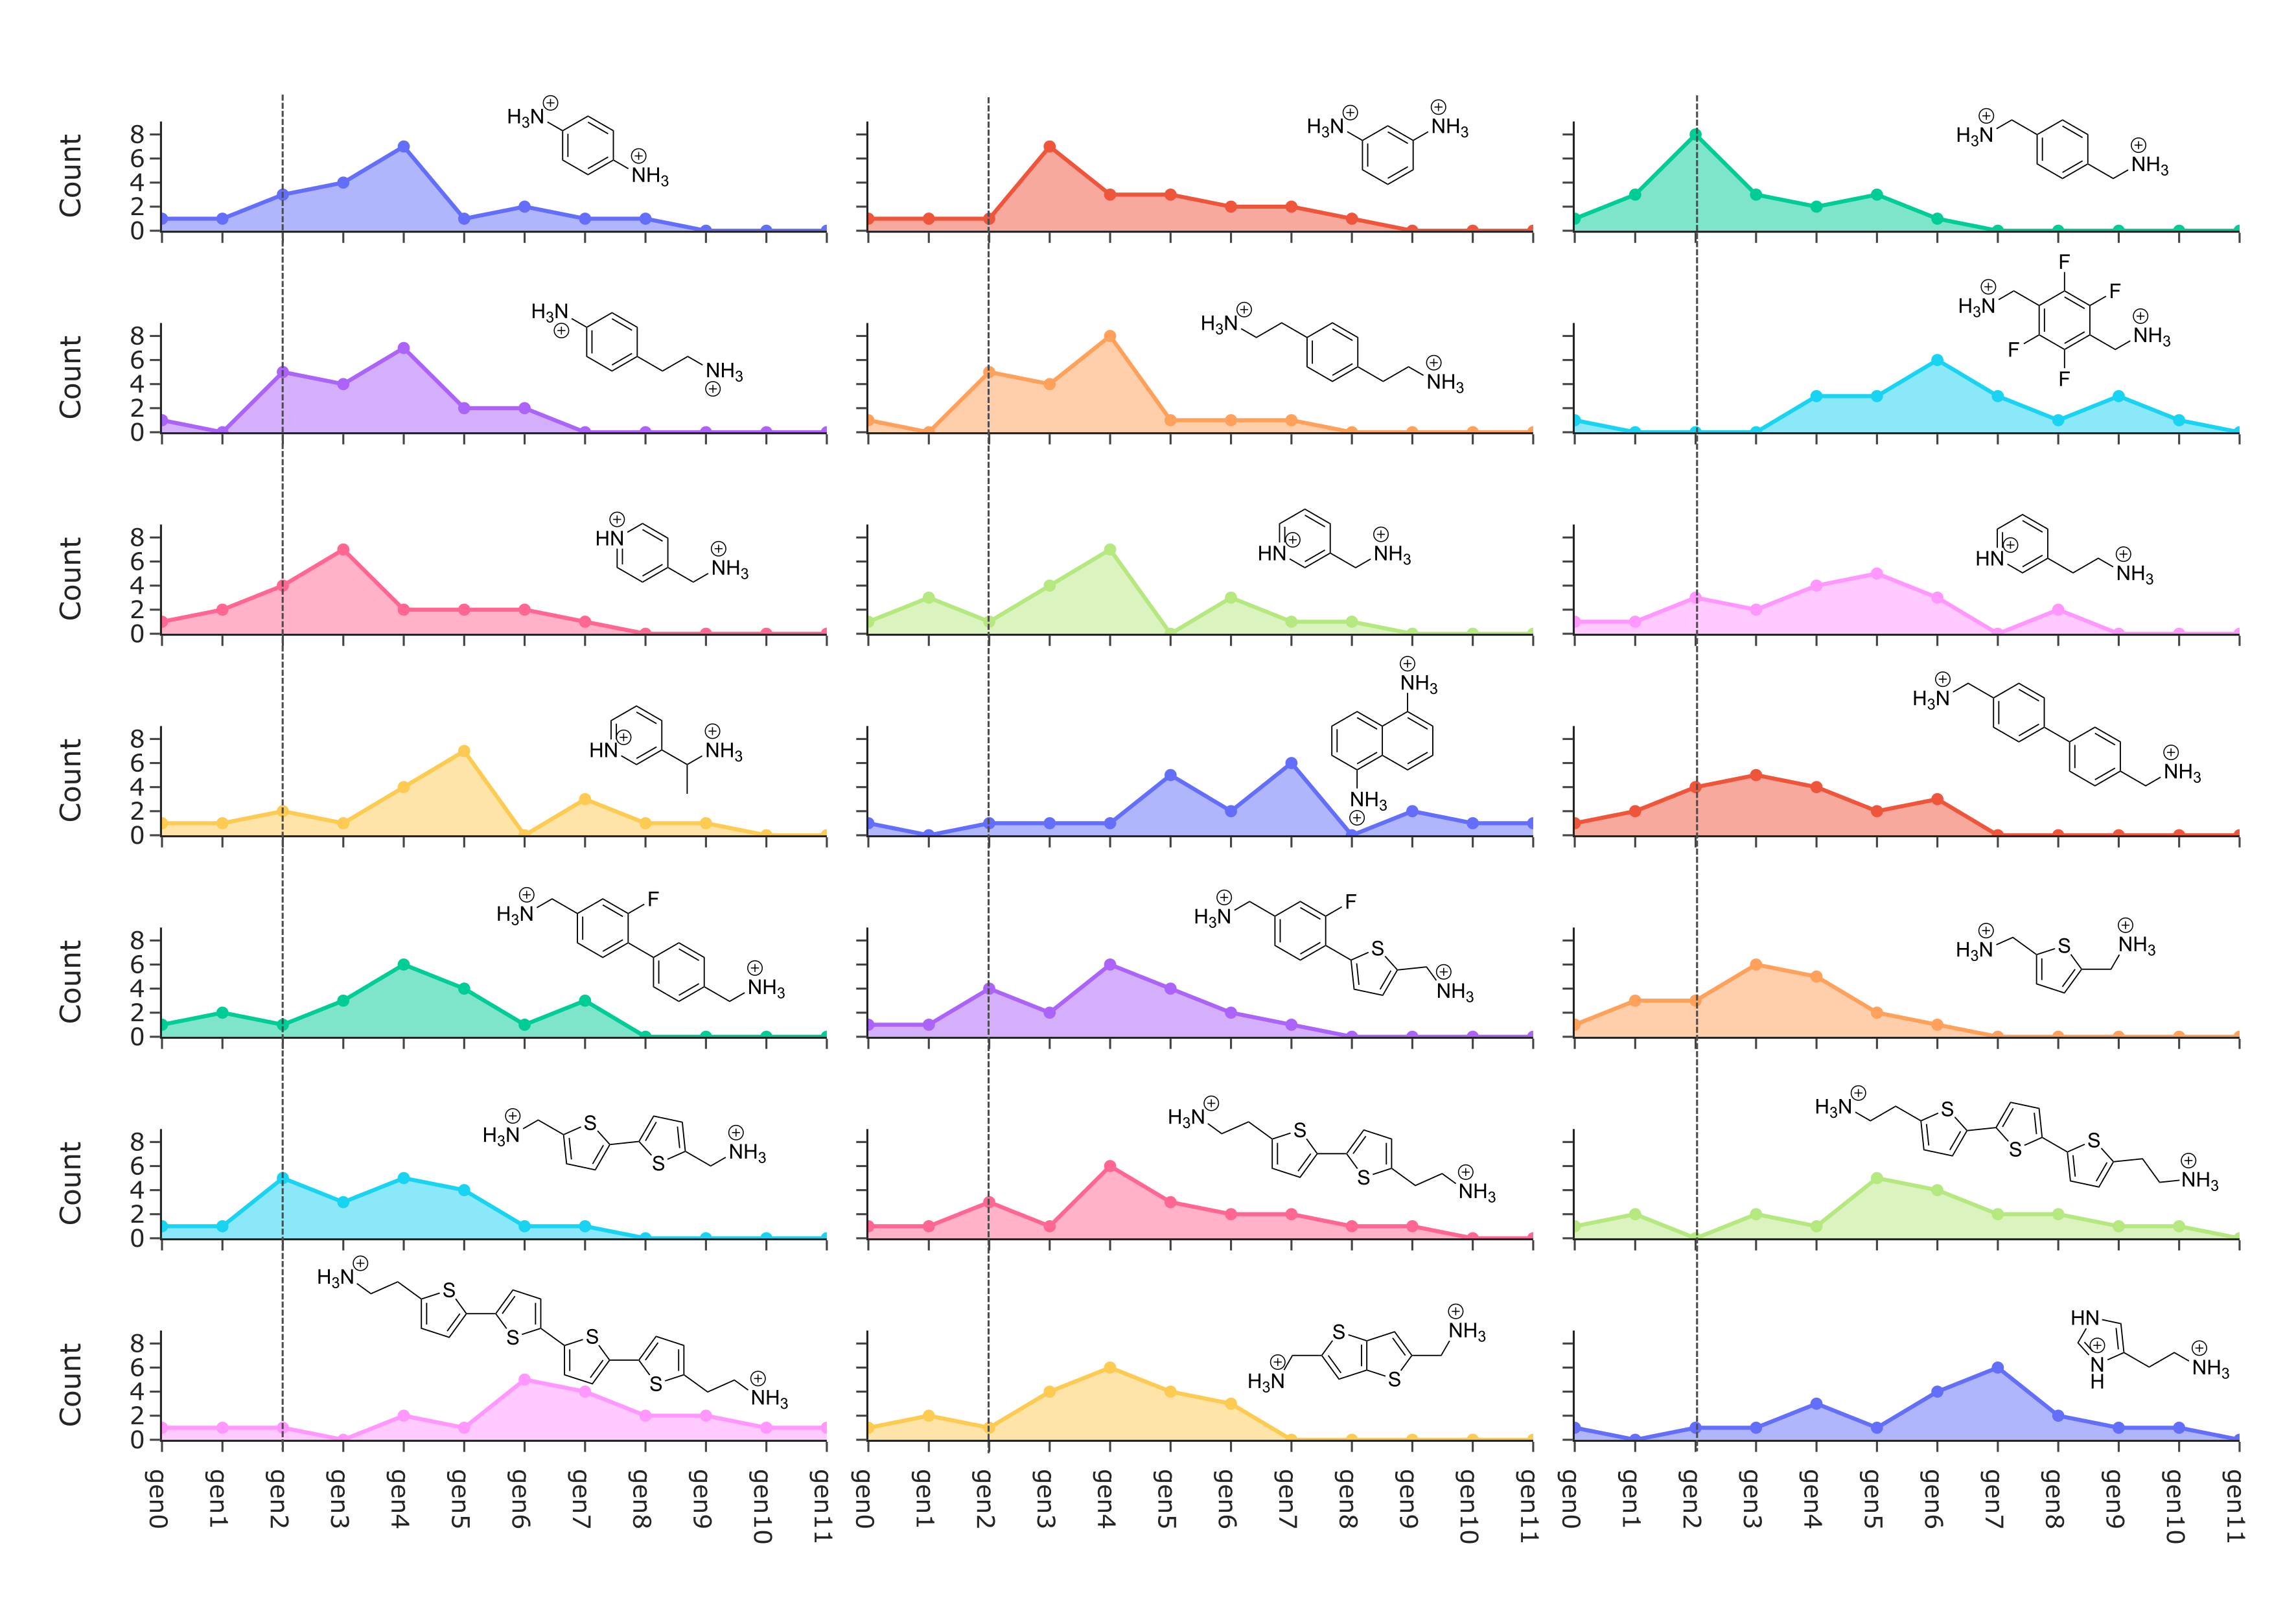
\includegraphics[width=\textwidth]{figures/methodology/figure3-8.png}
    \caption{Rationale for selection of PDMA as the generation $G_0$ organic spacer.}
    \label{fig:figure3.9}
\end{figure}


\textbf{Frontier level calculation of organic spacers}

The 3D molecular structures of organic spacers were generated from SMILES string using the RDKit library, which efficiently converts the molecular graph representations into 3D coordinates. Conformational sampling was conducted assuming the isolated, gas-phase configurations of the spacers, independent of their incorporation into the 2D perovskite structure. 

DFT calculations were performed using Gaussian 09 package with the B3LYP functional and 6-31G** basis set to calculate the energy levels of the HOMO and LUMO.

\textbf{Hybrid Perovskite Structure Generation}

The hybrid perovskite structures were constructed by inserting the organic spacers into a PbI$_4$-based inorganic framework. Initial conformations of the organic spacers were visualized in Avogadro and adjusted according to literature-reported configurations to reflect their likely conformations within the 2D perovskites. Specific modifications include: 

(1) Ensuring the linearity of linker groups to reduce aggregation effects observed in isolated forms. 

(2) Constraining rotations of linked aromatic rings to reflect dihedral angles typically found in hybrid perovskites, which are smaller than those in the isolated gas phase. For instance, benzene-benzene linkages were assigned a dihedral angle of 20°; thiophene-thiophene and thiophene-benzene linkages were constrained to 0°.

A $2\times2\times1$ supercell of PbI$_6$ octahedra was employed (each unit cell containing four organic spacers and four PbI$_4$ units), starting with an ideal cubic configuration in inorganic layers. Organic spacers are aligned along the lattice c direction, with two ammonium tethering groups intercalated within the cavities formed by the PbI$_6$ octahedra. Organic spacers are arranged in herringbone (out-of-phase) configuration. This configuration was chosen as it is frequently observed in experimental studies, with minimal influence on the electronic structure compared to other configurations. Interlayer distances between neighbouring PbI$_4$ layers were modulated according to spacer length, ensuring realistic structural representation. The framework was built programmatically using a combination of RDKit and pymatgen.

\begin{figure}[ht]
    \centering
    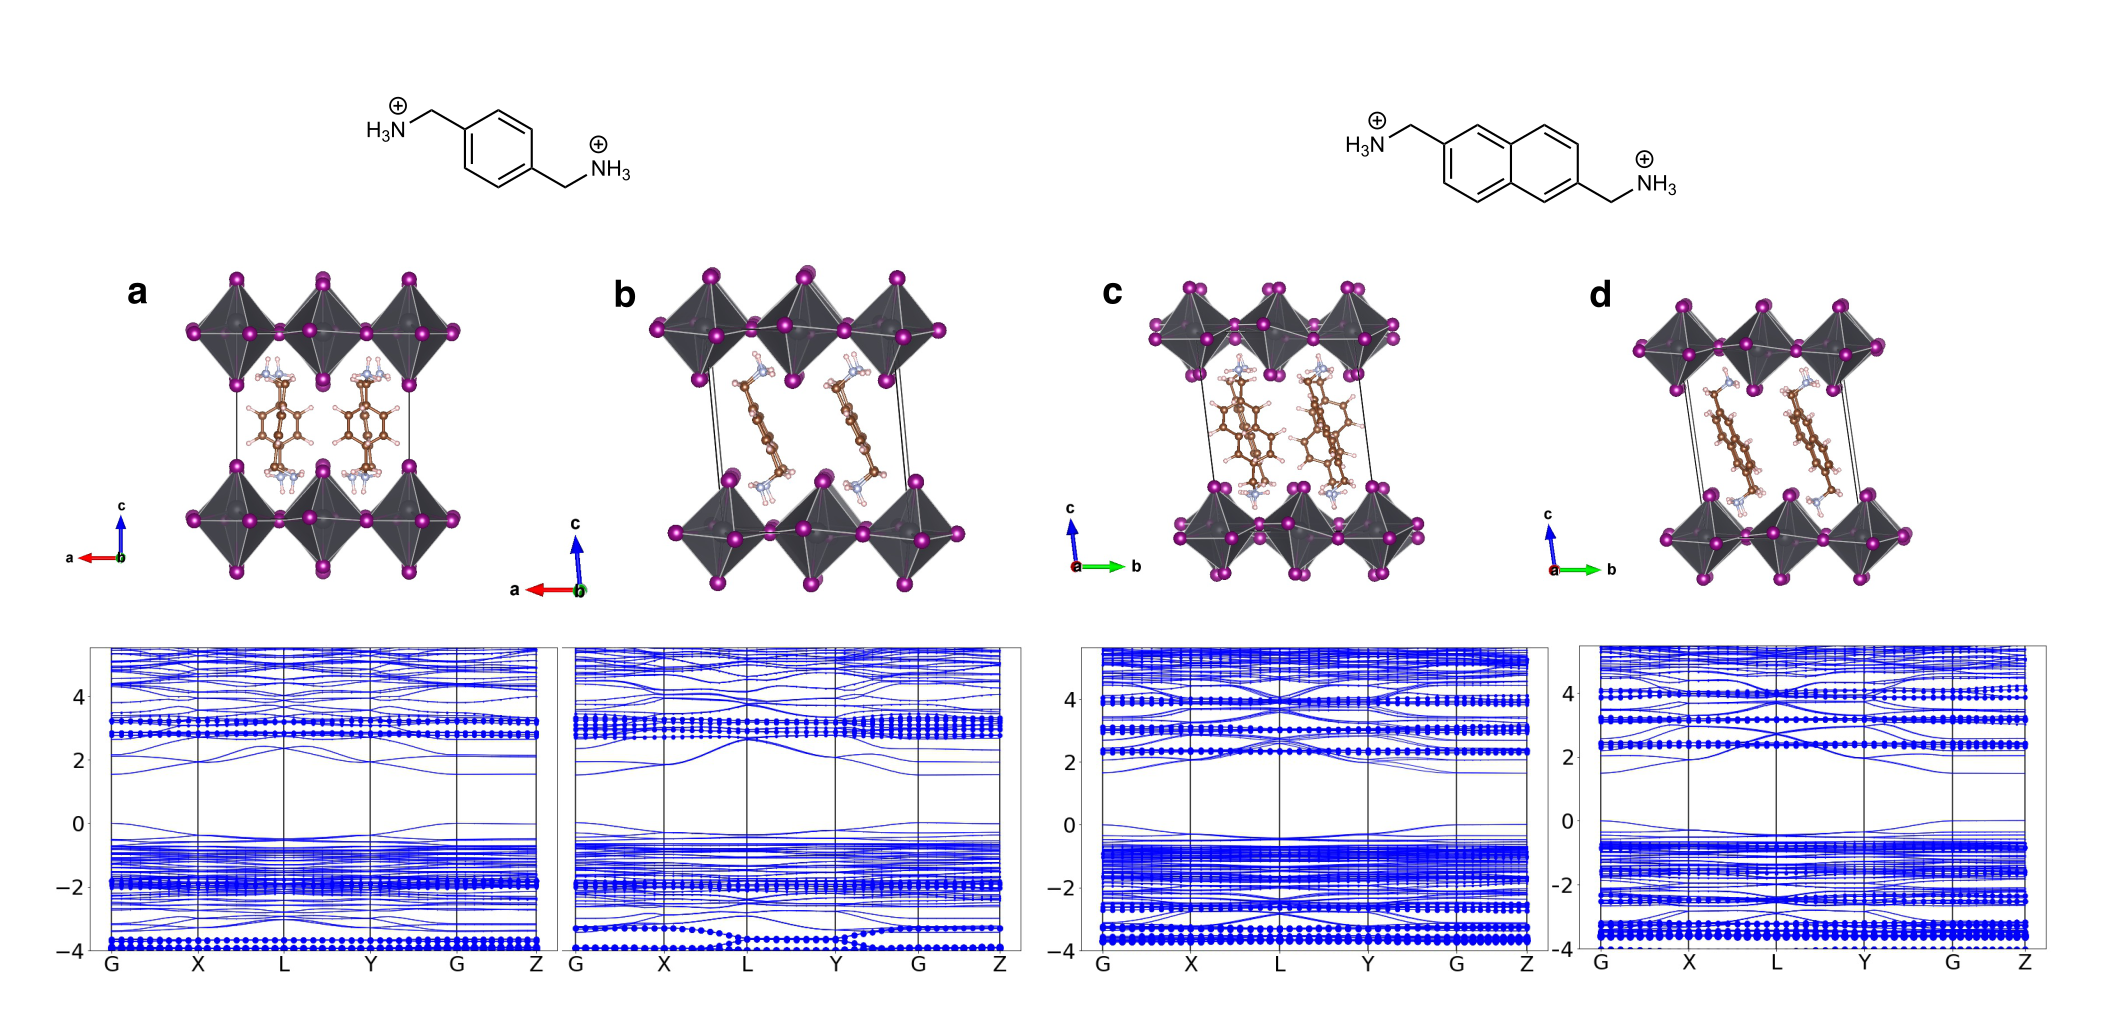
\includegraphics[width=\textwidth]{figures/methodology/figure3-10.png}
    \caption[Crystal structures and band structures of DJ perovskites with different organic spacer packing arrangements.]{Crystal structures and band structures of DJ perovskites with different organic spacer packing arrangements. Two example spacers are shown. Panels \textbf{a} and \textbf{c} illustrate out-of-phase (herringbone) packing, while \textbf{b} and \textbf{d} show in-phase packing.}
    \label{fig:figure3.10}
\end{figure}

Figure \ref{fig:figure3.10} shows a comparison between different packing pattern of organic spacers and their influence on the energy level in 2D perovskites. Figure \ref{fig:figure3.10}a and c shows the out-of-phase (herringbone) arrangement of organic spacers. This configuration is commonly observed in reported 2D perovskites, and our DFT calculation indicate this type of packing leads to minimal dispersion of molecular orbitals. Figure \ref{fig:figure3.10}b and d shows the in-phase arrangement, a configuration typically found in oligomer thiophene-based spacers. Our DFT calculation indicate that the molecular orbitals exhibit sizable dispersion ($\sim0.7$ eV as observed in this study), consistent with previous reports attributing this behaviour to electronic coupling among tightly packed adjacent organic spacers\cite{RN2}. Notably, one study indicates that out-of-phase configurations are energetically favoured\cite{RN41}. For consistency, we adopt the out-of-phase packing pattern across all structures. We anticipate that this in-plane dispersion of molecular orbitals will not affect our proposed final candidates for energy level alignment type Ib, IIa, and IIb, as this dispersion primarily broadens the organic frontier levels without shifting their centres.

\textbf{Perovskite Structure Relaxation}

DFT-based structure relaxations were performed using the Vienna Ab initio Simulation Package (VASP) with the Perdew-Burke-Ernzerhof (PBE) functional and projector augmented wave (PAW) pseudopotentials. Grimme’s DFT-D3 dispersion correction with zero damping was included to account for van der Waals interactions critical to layered perovskites. Relaxation was conducted in two steps: 

(1) A preliminary relaxation with a loose reciprocal density of 64 (resulting in k-point grids such as $1\times1\times1$ or $1\times1\times2$, depending on the lattice parameters along the c-axis). 

(2) A tighter relaxation with a reciprocal density of 300 (resulting in k-point grids such as $3\times3\times2$, $3\times3\times3$, or $3\times3\times4$). Convergence criteria required an energy difference per atom below $5\times10^{-6}$ eV.

\textbf{Electronic Structure Calculations}



To investigate the electronic properties of 2D perovskites, spin-orbit coupling (SOC) was included due to the significant relativistic effects in Pb-based compounds. The following workflow addressed the known limitations of commonly used functionals in predicting bandgap values and ensure alignment with experimental data: 

\begin{enumerate}
    \item Band structure shape identification: The band structure across the Brillouin zone was initially calculated using the PBE+SOC functional. This functional effectively captures the qualitative shape of the band structure but is known to underestimate the bandgap for perovskite materials. The results provided a foundational map of the electronic band dispersion. 

    \item Accurate bandgap calculation at representative points: To obtain accurate bandgap values, the HSE06+SOC hybrid functional was applied at critical points in the Brillouin zone ($\Gamma$ and Z). This method corrects the bandgap underestimation of PBE+SOC, ensuring quantitative agreement with experimental values. For structures with interlayer distances below 5 $\AA$, calculations were performed at both $\Gamma$ and Z points to capture the dispersion of inorganic bands from $\Gamma$ to Z. For larger interlayer distances (greater than 5 $\AA$), calculations were focused on the $\Gamma$ point only, as the dispersion becomes negligible. A Hartree-Fock exchange (HF) percentage of 40\% was used in the HSE06+SOC calculations, yielding bandgap values with a deviation of only 0.05 eV from experimental results. 

\begin{figure}[ht]
    \centering
    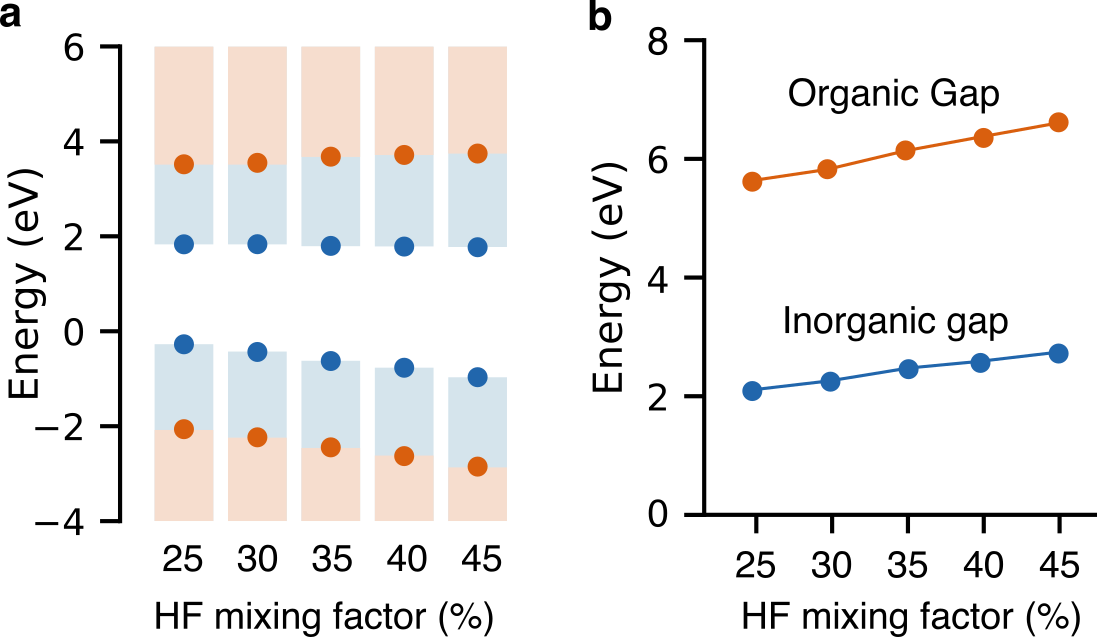
\includegraphics[width=0.75\textwidth]{figures/methodology/figure3-11.png}
    \caption[Effect of Hartree–Fock (HF) mixing factor on the calculated energy levels of organic and inorganic components in DJ-phase perovskites with the G$_0$ molecule (PDMA).]{Effect of Hartree–Fock (HF) mixing factor on the calculated energy levels of organic and inorganic components in DJ-phase perovskites with the G$_0$ molecule (PDMA). \textbf{a} Variation in energy level alignment with increasing HF mixing. \textbf{b} Evolution of the organic and inorganic energy gaps as a function of HF mixing factor.}
    \label{fig:figure3.11}
\end{figure}

\begin{figure}[ht]
    \centering
    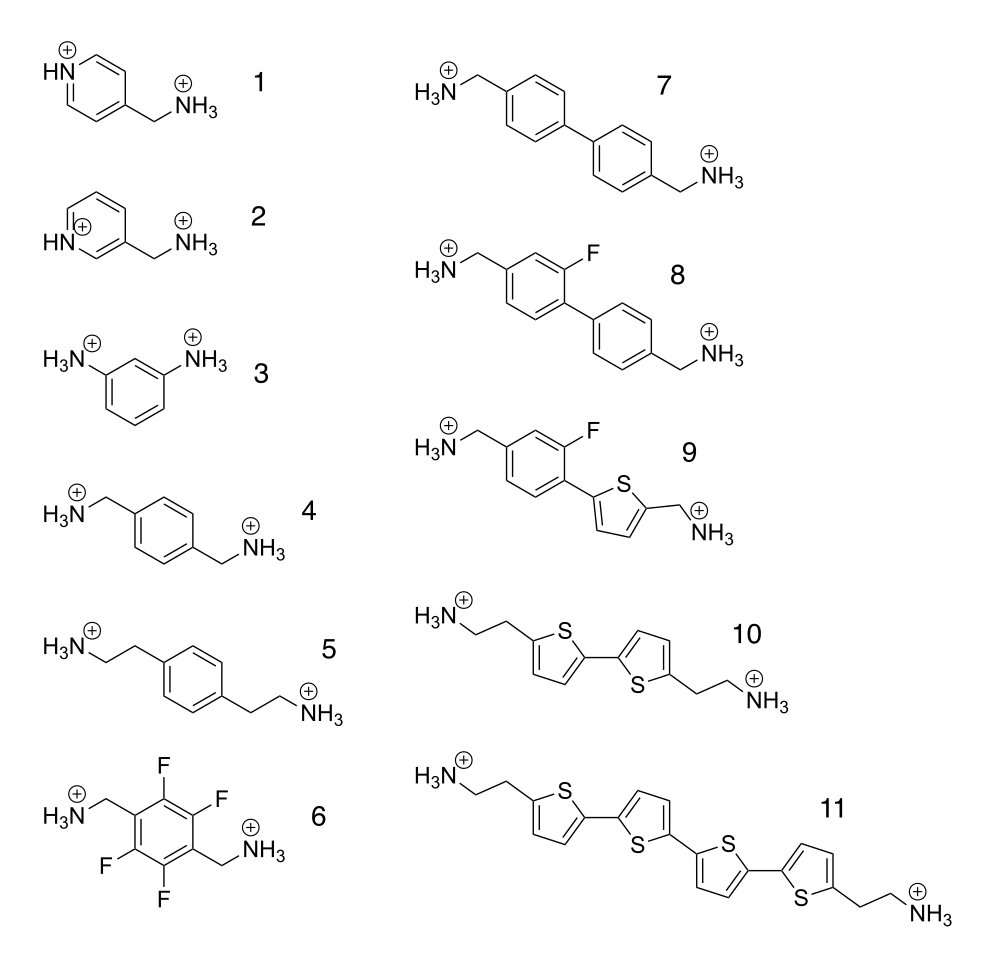
\includegraphics[width=0.6\textwidth]{figures/methodology/figure3-12.png}
    \caption{Reported organic spacers for which experimental bandgap values have been measured in the corresponding DJ perovskites.}
    \label{fig:figure3.12}
\end{figure}

\begin{table}[!ht]
    \centering
    \caption[Comparison of bandgap values calculated using HSE + SOC, HF=40\% and reported experimental values.]{Comparison of bandgap values calculated using HSE + SOC, HF=40\% and reported experimental values. Compound IDs correspond to the organic spacers listed in Figure \ref{fig:figure3.12}.}\label{table:table3.1}
    \begin{tabular}{|l|l|l|}
        \hline
        \textbf{Compound} & \textbf{Calculation (eV)} & \textbf{Experiment (eV)} \\  \hline
        1 & 2.42 & -\cite{RN31} \\ \hline
        2 & 2.26 & 2.34\cite{RN31} \\ \hline 
        3 & 2.39 & 2.42\cite{RN33} \\ \hline
        4 & 2.56 & 2.44\cite{RN86}, 2.42\cite{RN34} \\ \hline 
        5 & 2.42 & 2.46\cite{RN86}, 2.43\cite{RN95} \\ \hline 
        6 & 2.57 & 2.58\cite{RN95} \\ \hline
        7 & 2.38 & 2.52\cite{RN84} \\  \hline
        8 & 2.56 & 2.42\cite{RN84} \\  \hline 
        9 & 2.56 & 2.39\cite{RN84} \\  \hline
        10 & 2.79 & -\cite{RN41} \\ \hline 
        11 & 2.38 & 2.38\cite{RN38} \\ \hline 
    \end{tabular}
\end{table}

\begin{table}[!ht]
    \centering
    \caption[Effect of HF mixing factor on the calculated bandgap values of DJ perovskites.]{Effect of HF mixing factor on the bandgap values of DJ perovskites. Compound IDs correspond to the organic spacers listed in Figure \ref{fig:figure3.12}.}
    \label{table:table3.2}
    \begin{tabular}{|l|l|l|}
        \hline
          & \textbf{Compound 2 (eV)} & \textbf{Compound 4 (eV)} \\ \hline
        \textbf{Experiment} & 2.34\cite{RN31} & 2.44\cite{RN86}, 2.42\cite{RN34} \\ \hline
        \textbf{25\%} & 1.82 & 2.12 \\ \hline
        \textbf{30\%} & 1.97 & 2.26 \\ \hline
        \textbf{35\%} & 2.11 & 2.41 \\ \hline
        \textbf{40\%} & 2.26 & 2.56 \\ \hline
        \textbf{45\%} & 2.42 & 2.71 \\ \hline
    \end{tabular}
\end{table}

    Figure \ref{fig:figure3.11} shows the impact of mixing factor on the organic frontier levels in DJ perovskite. A range of mixing factors (25\% to 45\%) has been employed in earlier studies to match experimental bandgap values. In this work, we select a mixing factor of 40\%, as it yields the smallest average error of 0.05 eV. The mixing factor impacts the organic levels slightly more than the inorganic levels, though both follow very similar trends. This suggests that the energy level alignment type is unlikely to vary significantly for most proposed DJ perovskites. 

    Table \ref{table:table3.1} and \ref{table:table3.2} shows the bandgap of several existing DJ perovskites with different mixing factors, confirming the mixing factor of 40\% yield the smallest error compared to experimental value.

    \item Refined band structure across the Brillouin zone: To extend the high accuracy of HSE06+SOC calculations across the entire Brillouin zone without incurring the prohibitive computational cost, a scissoring technique was applied. The band structure obtained from PBE+SOC was adjusted using the band edges calculated at the $\Gamma$ and Z points with HSE06+SOC. The scissoring operation aligned the PBE+SOC-derived band structure with the inorganic band edge and organic frontier orbital levels predicted by HSE06+SOC, providing a consistent, high-fidelity representation of the electronic structure.
\end{enumerate}



\textbf{High-throughput framework}

The high-throughput DFT calculations for both organic spacers and hybrid perovskite structures were conducted on the Gadi supercomputer, utilizing a workflow based on the Materials Project (MP) input parameter template. The MP standards are widely recognized as the minimal benchmark in the field of DFT calculations, ensuring reproducibility and consistency across studies. These parameters are particularly suitable for capturing the general structural and electronic properties of a wide range of materials.

To meet the specific demands of hybrid perovskite systems, which are characterized by strong spin-orbit coupling, van der Waals interactions, and low-symmetry structures, we further refined and tightened the computational parameters. Key refinements included:

\begin{itemize}
    \item Energy Convergence Criterion: The MP default for electronic energy convergence (EDIFF) is $5\times10^{-5}$ eV per calculation. For our study, we set a stricter threshold of $5\times10^{-6}$ eV per atom to ensure reliable energy differences for low-symmetry perovskite structures.
    \item Plane-Wave Cutoff Energy: While the MP standard cutoff energy is typically 520 eV, we adjusted this to 480 eV, as testing showed that this value-maintained accuracy for perovskite systems while optimizing computational efficiency.
    \item Reciprocal Space Sampling: For initial structural relaxation, we used the default MP reciprocal density of 64 (resulting in k-point grids such as $1\times1\times1$ or $1\times1\times2$, depending on the c-axis lattice parameter). For final relaxation and electronic property calculations, we increased the reciprocal density to 300, corresponding to dense k-point grids such as $3\times3\times3$, $3\times3\times2$, or $3\times3\times4$. This stricter k-point sampling ensured accurate modelling of structural distortions and electronic properties in the layered perovskites.
    \item Dispersion Corrections: To account for van der Waals interactions in layered systems, Grimme’s DFT-D3 dispersion correction with zero damping was included. This refinement is critical for accurately describing interlayer interactions in 2D perovskites.
\end{itemize}

The high-throughput framework was automated using the pymatgen library to generate VASP input files and parse outputs, enabling systematic and efficient exploration of $\sim3,000$ organic spacers and $\sim400$ hybrid perovskite structures. By building on the minimal standards established by the Materials Project and incorporating additional refinements specific to perovskites, we ensured that our computational results met the highest standards of accuracy and reliability for this material system.

\section{Machine Learning}\label{section:section3-4}

All machine learning tasks in this thesis were conducted using the Scikit-learn library in Python. This included data preprocessing, dimensionality reduction, training of regression and classification models, and extraction of feature coefficients for model interpretation.

\textbf{Dimensional reduction for chemical space visualization}

To visualize the chemical space of organic spacers, we employed unsupervised learning techniques for dimensionality reduction. We compared Principal Component Analysis (PCA), a linear dimensionality reduction method, with t-distributed stochastic neighbour embedding (t-SNE), a nonlinear technique designed to capture complex high-dimensional data structures in a lower-dimensional space. While PCA provided an initial overview, the resulting plots exhibited significant overlap between data points, limiting its ability to distinguish between structurally diverse spacers. Consequently, we selected t-SNE for its superior capability in preserving local and global relationships within the data.

Each spacer was represented numerically using a 12-dimensional fingerprint vector that encodes key structural and chemical features relevant to our analysis. The dataset, comprising $\sim20,000$ fingerprints corresponding to $\sim4\times10^6$ spacers generated across generations $G_0$ to $G_6$, was subjected to t-SNE analysis. We utilized a perplexity of 40 to balance the consideration of local and global data structures, optimizing the algorithm’s sensitivity to both densely and sparsely populated regions of the chemical space.

The output of this process was a set of two-dimensional coordinates that effectively represent the high-dimensional chemical space of the spacers, enabling clear visualization of structural similarities and differences across spacer generations.

\textbf{Data Collection and Input Features}

The dataset comprised high-throughput computational data on 3,239 organic molecules across generations $G_0$ to $G_4$ with varying structural and electronic properties. The target properties for prediction were the highest occupied molecular orbital (HOMO) and lowest unoccupied molecular orbital (LUMO) energies of isolated organic spacers.

The input features were 12-digit organic fingerprints, which are highly relevant to the target properties due to their comprehensive representation of molecular descriptors. These fingerprints capture the chemical, electronic, and structural characteristics of the organic molecules, providing a robust basis for predictive modelling. Correlation analysis revealed minimal redundancy among the features, negating the need for additional feature selection methods.

To ensure comparability across features, all input data were normalized to have zero mean and unit variance using the StandardScaler module in the Scikit-learn library. This normalization step mitigates bias arising from differences in feature scales, thereby optimizing model performance.

\textbf{Model Training and Validation}

The data was partitioned into training and test sets using an 80:20 random split, ensuring an unbiased evaluation of model performance. The training data was further subjected to five-fold cross-validation to ensure robustness and to avoid overfitting.

\begin{table}[ht]
\centering
\caption{Hyperparameters for various regression ML models for HOMO and LUMO predictions.}
\begin{tabular}{|l|l|l|}
\hline
\textbf{Method} & \textbf{HOMO} & \textbf{LUMO} \\ \hline
Linear regression & no hyperparameter & no hyperparameter \\ \hline
Lasso regression & $\alpha = 0.001$ & $\alpha = 0.001$ \\ \hline
Ridge regression & $\alpha = 1.0$ & $\alpha = 5.0$ \\ \hline
Elastic net regression & $\alpha = 0.001$ & $\alpha = 0.001$ \\ \hline
SVM (kernel = linear) & $C=20, \epsilon=0.1$ & $C=10, \epsilon=0.1$ \\ \hline
SVM (kernel = rbf) & $C=10, \epsilon=0.1$ & $C=10, \epsilon=0.1$ \\ \hline
SVM (kernel = poly) & $C=1, \epsilon=0.1$ & $C=1, \epsilon=0.1$ \\ \hline
K neighbours regressor & $n\_neighbours=7$ & $n\_neighbours=7$ \\ \hline
Random forest regressor & $n\_estimators=100$ & $n\_estimators=100$ \\ \hline
\end{tabular}

\label{table:table3.3}
\end{table}

We evaluated the performance of several machine learning models implemented in the Scikit-learn library. Grid search with cross-validation was used to identify optimal hyperparameters for each model, as summarized in Table \ref{table:table3.3}.

All models with optimal hypterparameters were evaluated using 15-fold cross-validation (cv=15) implemented via Scikit-learn’s cross\_validate function to ensure consistent and reliable estimation of fitting error.

\textbf{Performance metrics}

The models were evaluated based on two key metrics: 

(1) R$^2$ Score. Quantifying the proportion of variance explained by the model, with higher values indicating better fit.

\begin{equation}
    R^2 = 1 - \frac{SS_{\text{RES}}}{SS_{\text{TOT}}} = 1 - \frac{\sum_i (y_i - \hat{y}_i)^2}{\sum_i (y_i - \bar{y})^2}
\end{equation}

(2) Root Mean Squared Error (RMSE): Providing an absolute measure of predictive accuracy, with lower values indicating smaller residual errors.

\begin{equation}
RMSE = \sqrt{\frac{\sum\limits_{i=1}^{n} (\hat{y}_i - y_i)^2}{n}}
\end{equation}

Both metrics were calculated for the training and test datasets. The results demonstrated excellent predictive performance for both linear ($\sim0.95$) and non-linear models ($\sim0.99$). This level of performance suggests that the relationships in the data are well captured by the chosen models, obviating the need for more advanced techniques, such as deep learning, for this study.

LASSO regressions were selected as the optimal model due to their decent predictive accuracy and interpretability. The importance of each input feature, both normalized coefficient and unnormalized coefficient, was analysed to verify the contribution of the organic fingerprint descriptors to the target predictions.

\textbf{SHAP value analysis.}


To interpret the feature importance and contribution of individual organic descriptors in predicting HOMO/LUMO, we employed SHapley Additive exPlanations (SHAP) values. SHAP values provide a game-theoretic approach to quantify each feature’s impact on the model’s output.

Unlike the conventional approach of using the average feature value as the reference point, we calibrated all SHAP values using a baseline molecule from Generation 0. This calibration allowed us to directly compare feature contributions relative to a chemically meaningful reference, facilitating more insightful interpretations. 

The SHAP values were computed and visualized using the SHAP library in Python.

\section{Synthesis feasibility screening}\label{section:section3-5}


\textbf{PubChem existence}

The presence of an organic spacer in the PubChem database was used as a proxy for synthetic accessibility. PubChem is a comprehensive chemical information repository, widely used to assess the availability and feasibility of molecular synthesis.

The neural form of organic spacers is converted to SMILES format to ensure compatibility with PubChem’s search algorithms. The neutral SMILES string was used to retrieve chemical information via the pubchempy library, which interacts with the PubChem API. Key identifiers, including the compound identifier (CID) and International Union of Pure and Applied Chemistry (IUPAC) name, were extracted for each molecule.

Due to limitations on the number of requests allowed by the PubChem API, this process was computationally slower than other components of the high-throughput pipeline. Therefore, synthetic accessibility screening was limited to the generations $G_0-G_4$ molecules, totalling approximately $\sim10^4$ candidates.

\textbf{2D structure formability}

The formability of a 2D perovskite structure was evaluated based on the spatial and chemical properties of hydrogen-donor nitrogen atoms within the organic spacers. Four descriptors were used to quantify the formability of the candidate spacers:
\begin{enumerate}

    \item Steric hindrance index (STEI): This descriptor measures the steric hindrance around a target nitrogen atom, calculated as the inverse sum of the cubed distances to all other atoms in the molecule:
    \begin{equation}
        \text{STEI}_{N_i} = \sum_{j=1}^n \frac{1}{\left(d_{N_i - \text{Atom}_j}\right)^3}
    \end{equation}
A larger STEI indicates a higher density of nearby atoms, increasing steric hindrance and potentially reducing the likelihood of forming hydrogen bonds with the inorganic framework.
    \item Eccentricity: Eccentricity quantifies the molecular shape with respect to a nitrogen atom, measuring the longest distance between the nitrogen and any other atom in the molecule:
    \begin{equation}
        \text{Eccentricity}_{N_i} = \max\left(d_{N_i - \text{Atom}_j}\right)
    \end{equation}

Larger eccentricity values correspond to more elongated molecules, which are favorable for forming 2D perovskite layers.
	\item Number of rotatable bonds (NumRot): This descriptor reflects the flexibility of the ammonium group tethered to the nitrogen atom, calculated as the minimum distance from the nitrogen to the nearest atom in the conjugated backbone:

    \begin{equation}
        \text{Num\_Rot}_{N_i} = \min\left(d_{N_i - \text{RingAtom}_j}\right)
    \end{equation}
A higher number of rotatable bonds improves flexibility, facilitating the anchoring of the organic spacer to the inorganic framework.
	\item N-N pair distance (Dis$_{NN}$): This descriptor measures the spatial separation between two nitrogen atoms in a molecule:
    \begin{equation}
        \text{Dis}_{N_i - N_j} = \frac{1}{\left(d_{N_i - N_j}\right)^2}
    \end{equation}
A smaller value indicates a larger distance, reducing repulsive interactions and enhancing structural stability in 2D perovskite layers.
\end{enumerate}

	
All descriptors were computed from the distance matrix of organic spacers, which is obtained using RDKit library in python. Briefly, all hydrogen-donor nitrogen atoms were identified in the distance matrix, and their corresponding descriptors were calculated using the equation above.

A boundary-based approach was applied to screen out unsuitable organic spacers. Decision boundaries were defined using the properties of known, successfully synthesized spacers from the literature. Molecules failing to meet the criteria for any of the four descriptors were excluded from further consideration. This systematic screening ensured that only candidates with favourable synthetic accessibility and structural formability proceeded to the subsequent stages of analysis.

    \chapter[High-Throughput Calculation and Machine Learning Predictions]{High-Throughput Calculation and Machine Learning Predictions} \label{c:result-1} 

In this chapter, we describe the generation of hypothetical organic spacers and the subsequent prediction of their properties using a combined high-throughput DFT approach and machine learning techniques. Section \ref{section:section4-1} outlines the systematic expansion of the organic spacer library through molecular morphing operations. Section \ref{section:section4-2} presents general physical insights derived from high-throughput DFT calculations. Sections \ref{section:section4-3} and \ref{section:section4-4} discuss the selection and evaluation of machine learning models, highlighting their predictive performance and their role in extracting structure-property relationships.


\section{Molecular generation for chemical space expansion}\label{section:section4-1}

\subsection{Morphing operation}

\begin{figure}[htbp]
    \centering
    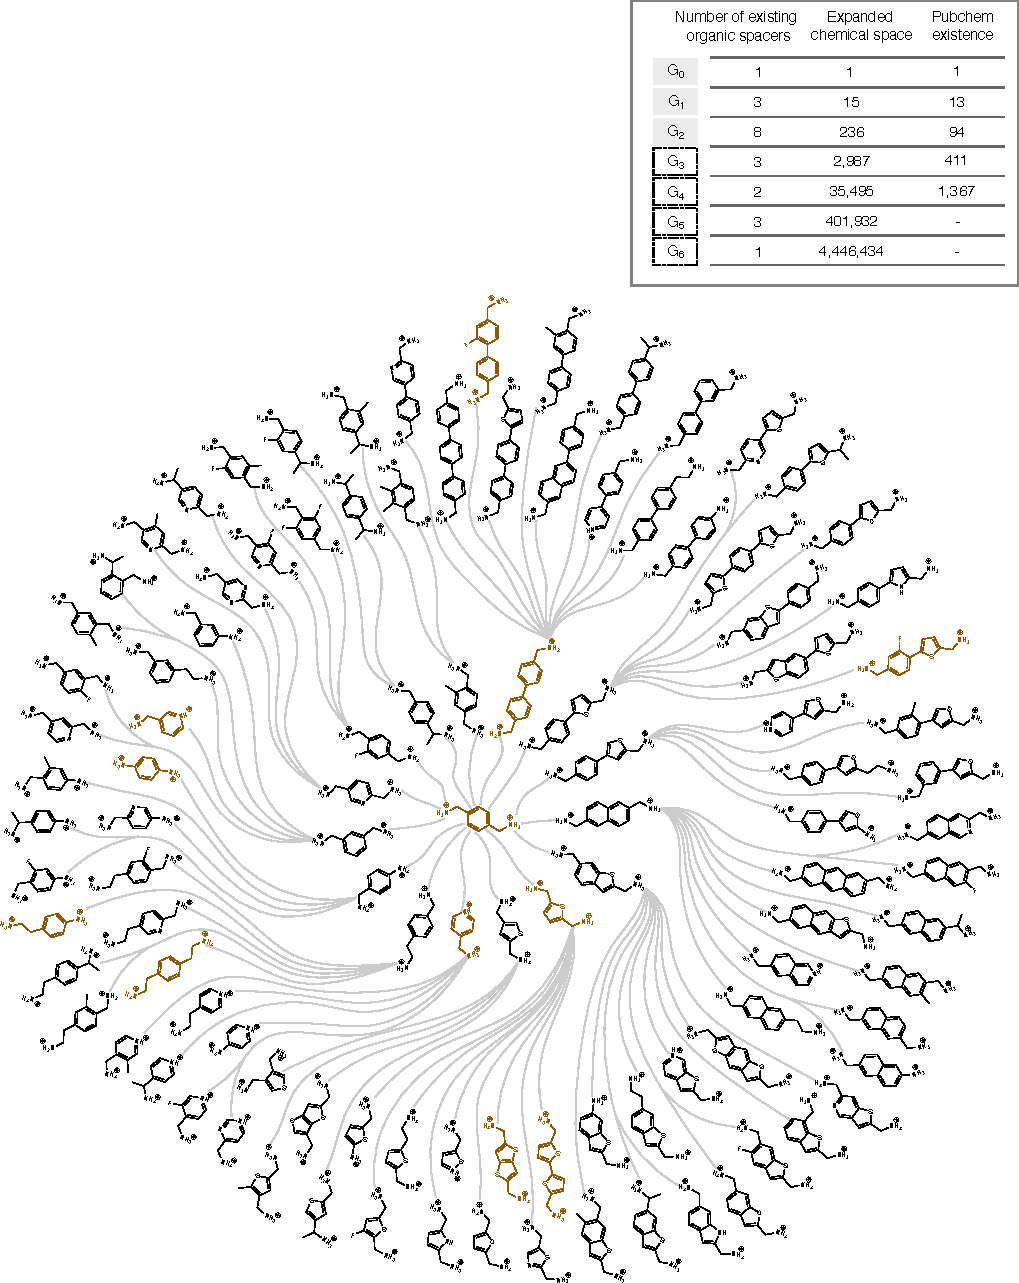
\includegraphics[width=\textwidth]{figures/HT-ML/figure4-1.pdf}
    \caption{Scaffold tree plot illustrating the organic spacer generation process.}
    \label{fig:figure4.1}
\end{figure}

To systematically explore a broad and diverse chemical space, we employed a deterministic molecular morphing approach rather than stochastic molecular generation methods\cite{RN236,RN310}. This ensures controlled diversification while maintaining the chemical interpretability of the generated spacers. As detailed in Chapter \ref{c:method}, each spacer is represented by a 12-digit fingerprint vector, which encodes key molecular features such as $\pi$-conjugation, ammonium tethering, heteroatom substitution, and side-chain modifications. All the morphing operators are associated with organic desciptors in the molecular fingerprint (Table \ref{t:morphing1}). This approach enables the enumeration of structurally diverse yet chemically meaningful molecular variations, ensuring a comprehensive and uniform coverage of the chemical space.

We initiate the morphing process from PDMA (Generation 0, $G_0$), a well-characterized organic spacer\cite{RN34}. We iteratively apply 13 distinct morphing operators to introduce incremental modifications, systematically generating higher-order generations ($G_1-G_6$). The molecular generation process is illustrated in Figure \ref{fig:figure4.1}. All organic spacers in $G_0$ (centre core), $G_1$(first circle) are displayed. For $G_2$ (second and third circle), only representative structures with unique molecular fingerprints to maintain clarity. Experimentally reported molecules within $G_0-G_2$ are highlighted, while the inset table quantifies the exponential expansion of the chemical space, which increases from an initial set of 21 reported organic spacers to millions of hypothetical spacers within $G_0-G_6$.

\begin{table}[!ht]
    \centering
    \caption{List of organic descriptors and their associated morphing operators.}\label{t:morphing1}
    \begin{tabular}{|l|r|r|}
        \hline
        \textbf{Number} & \textbf{Morphing operation} & \textbf{Organic descriptor} \\  \hline
        1 & Benzene-thiophene ring exchange & five-membered ring \\ \hline
        2 & Ring linkage & ring linkage \\ \hline 
        3 & Ring fusion & ring fusion \\ \hline
        4 & Primary secondary amine exchange & number of primary amine \\ \hline 
        5 & Linker length increase & Linker length \\ \hline 
        6 & Linker length decrease & Linker length \\ \hline
        7 & Linker position change & linker position \\  \hline
        8 & Hetero-nitrogen substitution & hetero-nitrogen \\  \hline 
        9 & Fluorination & fluorination \\  \hline
        10 & Furan exchange & furan \\ \hline 
        11 & Pyrrole exchange & pyrrole \\ \hline 
        12 & Side chain on backbone & no. side chain on backbone \\ \hline  
        13 & Side chain on linker & no. side chain on linker \\ \hline
    \end{tabular}
\end{table}

The morphing operations yield progressively complex sets of organic spacers. For example, to incorporate five-membered ring backbones, we utilize a ring contraction operator that transforms benzene into thiophene, thereby diversifying the core molecular framework. This systematic expansion extends beyond commonly studied phenyl- and thiophene-containing families, encompassing a broader spectrum of heteroatom-substituted structures (e.g., F, O, N) and various side-chain modifications.

The 21 experimentally reported organic spacers were captured within generations $G_0-G_6$, and with comparable complexity in these generations, we enumerated 21,306 fingerprints, corresponding to 4,887,100 hypothetical organic spacers. To assess the chemical feasibility of the generated molecules, the neutral forms of the hypothetical spacers were cross-referenced against the PubChem database. Within generations $G_0-G_4$, where computational feasibility allowed exhaustive searches, $\sim10^3$ spacers were identified in PubChem, confirming that a subset of our generated structures aligns with known chemical compounds. This validates the chemical plausibility of the generated molecular space.

\subsection{Visualization of generated chemical space}

To provide an intuitive understanding of the distribution and structural diversity of the generated organic spacers, we employ a dimensionality reduction technique to visualize the chemical space. Since the molecular fingerprints exist in a 12-dimensional space, we utilize t-distributed stochastic neighbour embedding (t-SNE)\cite{RN551}, an unsupervised learning algorithm that transforms high-dimensional data into a two-dimensional representation while preserving the relative distances between structurally similar molecules.

\begin{figure}[htbp]
    \centering
    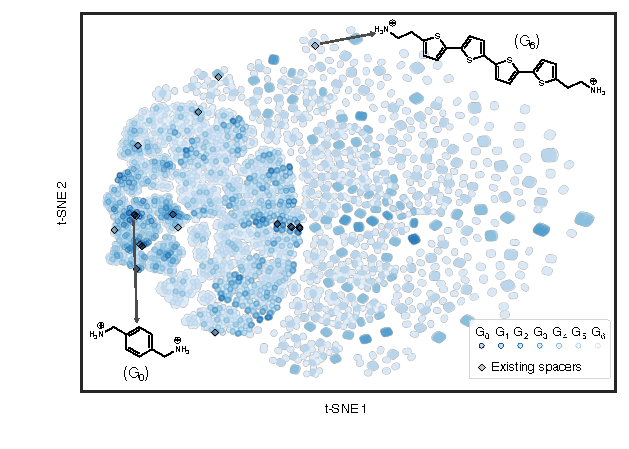
\includegraphics[width=0.8\textwidth]{figures/HT-ML/figure4-2.pdf}
    \caption{t-SNE representation of the generated chemical space containing the hypothetical organic spacers.}
    \label{fig:figure4.2}
\end{figure}

The resulting t-SNE map is shown in Figure \ref{fig:figure4.2}, representing $\sim2\times10^4$ unique fingerprints corresponding to $\sim4\times10^6$ organic spacers across generations $G_0-G_6$. Experimentally reported spacers are highlighted, with representative molecules from $G_0$ and $G_6$ explicitly labelled. The spatial organization of the t-SNE clusters reflects the underlying structural similarities among different spacers: closely grouped molecules share similar fingerprint features, while larger inter-cluster distances correspond to structurally dissimilar spacers.

Notably, among all reported spacers, the highest-generation example ($G_6$), AE4T\cite{RN38}, is distinctly separated from other spacers, reflecting its more complex structure. This visualization demonstrates that our generative workflow comprehensively covers the chemical space surrounding experimentally known spacers, including AE4T. Compared to traditional molecular datasets compiled from pre-existing databases, our approach ensures a more uniform and representative sampling, avoiding biases toward extreme or rare structures. By maintaining a balanced distribution of generated molecules, we enable reliable high-throughput calculations and robust machine learning predictions. As we will demonstrate later in this chapter, this curated dataset serves as a reliable foundation for training machine learning models, enhancing their ability to predict electronic properties with high accuracy.

\subsection{Descriptor-based visualization and cluster analysis}

\begin{figure}[htbp]
    \centering
    \includegraphics[width=\textwidth]{figures/HT-ML/figure4-3-1.pdf}
    \caption{Visualization of the chemical space with respect to organic descriptors in molecular fingerprint (Part 1).}
    \label{fig:figure4.3}
\end{figure}

\begin{figure}[htbp]
    \centering
    \ContinuedFloat
    \includegraphics[width=\textwidth]{figures/HT-ML/figure4-3-2.pdf}
    \caption{Visualization of the chemical space with respect to organic descriptors in molecular fingerprint (Part 2, continued).}
\end{figure}

To further examine the relationships between molecular descriptors and structural similarity, we present Figure \ref{fig:figure4.3}, which depicts the same t-SNE map but color-coded according to different molecular descriptors derived from the fingerprint vector. 
This visualization highlights key trends:
\begin{enumerate}
    \item Molecular spacers with similar descriptors cluster together, confirming that the fingerprint representation effectively captures structural relationships.
    \item The non-linear characteristic of t-SNE is well observed and it makes it easier to understand how t-SNE work. Note that the non-linearity organization of data points reflects the fundamental difference between t-SNE and principal component analysis (PCA). While PCA, a linear dimensionality reduction technique, is widely used in materials informatics, we found that it resulted in excessive overlap between structurally distinct molecules. By contrast, t-SNE preserves local structures more effectively, providing better differentiation of organic spacers.
\end{enumerate}

\begin{figure}[htbp]
    \centering
    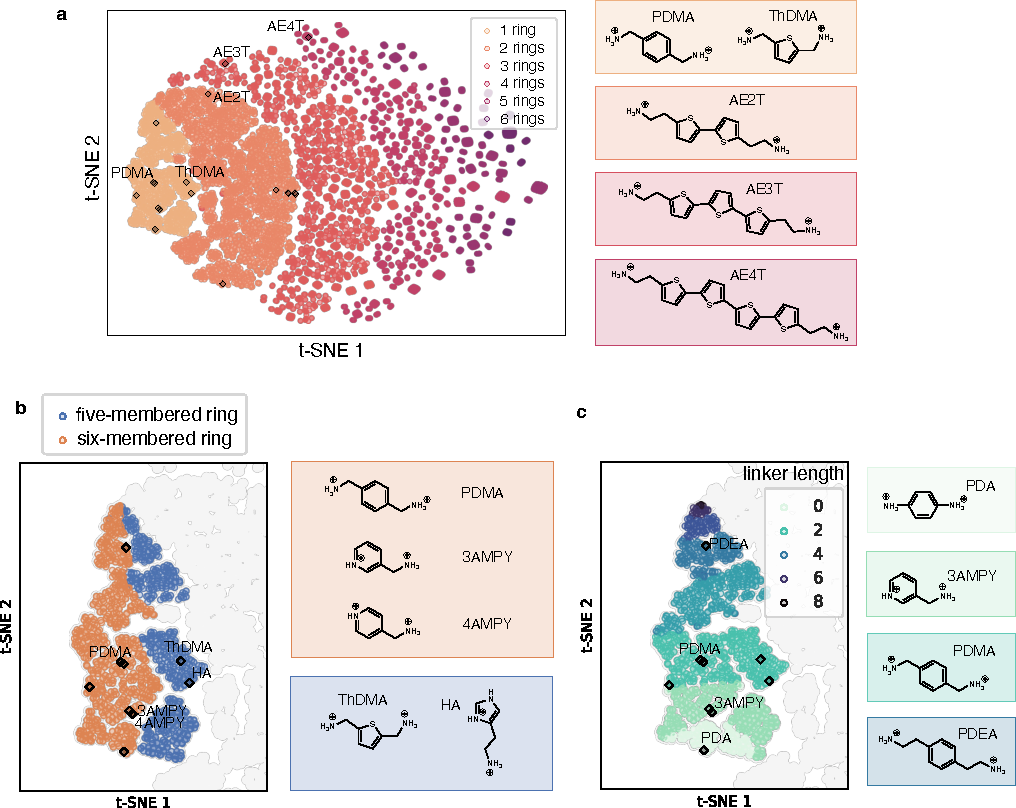
\includegraphics[width=\textwidth]{figures/HT-ML/figure4-4.pdf}
    \caption[Chemical space visualization of existing spacers.]{Chemical space visualization of existing spacers. \textbf{a} Complete chemical space. \textbf{b,c} Enlarged views highlighting spacers containing a single aromatic ring.}
    \label{fig:figure4.4}
\end{figure}


A deeper analysis of specific clusters within the t-SNE map is presented in Figure \ref{fig:figure4.4}, focusing on the existing organic spacers. The full distribution of the generated organic spacers is shown in Figure \ref{fig:figure4.4}a. A clear gradient is observed from left to right, reflecting increasing number of aromatic rings. Spacers such as PDMA and ThDMA, which contain a single aromatic ring and are widely used in 2D perovskites, cluster on the left side of the plot. On the other hand, highly conjugated organic spacers, such as the oligothiophene-based spacers (AE2T, AE3T, AE4T) are found progressively further to the right.

Figure \ref{fig:figure4.4} b,c provide focused views of subspaces containing spacers with a single aromatic ring. In \textbf{b}, molecules are colored by ring type, highlighting distinct clustering between five-membered ring and six-membered ring as conjugated backbones. In \textbf{c}, the same subset is colored by linker length. A spatial gradient is visible, with shorter linkers (e.g., PDA, linker length = 0) clustering in the top and longer linkers (e.g., PDEA, linker length = 4) spreading toward the bottom. This demonstrates that the fingerprint-based t-SNE projection effectively captures meaningful structural and functional diversity among known spacers.



\section{Influence of organic spacer structure on energy levels}\label{section:section4-2}

\subsection{DFT calculation of DJ perovskites}

To assess the impact of organic spacer selection on the electronic properties of DJ perovskites, we performed a detailed high-throughput DFT analysis on 261 DJ-phase perovskites. This dataset includes both experimentally reported spacers and hypothetical spacers from generations $G_0-G_2$ of our expanded chemical space. Model crystal structures were constructed by inserting organic spacers between the PbI$_4$ layers, with each unit cell containing four diammonium spacers and four PbI$_4$ units (see Chapter \ref{c:method} for computational details). 

\textbf{Organic spacer packing configurations}

In computational studies of DJ perovskites, two primary packing arrangements of organic spacers are typically assumed: in-phase and out-of-phase configurations. Unlike the inorganic sublattice, which undergoes significant structural distortions (such as octahedral tilting and bond-angle variations), the organic spacers exhibit minimal changes in packing pattern upon structural relaxation. This behaviour suggests that interactions between organic spacers and the inorganic layers, as well as interactions among the organic spacers themselves, are relatively weak, occurring primarily through hydrogen bonding and van der Waals interactions. Consequently, both in-phase and out-of-phase arrangements lead to well-converged structures, indicating that the energy difference between these configurations is small. This suggests a shallow energy landscape with respect to the relative alignment of organic spacers.

Despite the energetic similarity between different packing arrangements, our analysis revealed that the packing configuration has minimal influence on the energy level alignment. Therefore, to align with experimentally observed structures, all organic spacers were assign to arranged in herringbone (out-of-phase) configurations\cite{RN41}. The optimized geometries were computed at the DFT-PBE level. 

\textbf{Bandgap calibration and energy level alignment}

The energy level alignment between the organic frontier molecular orbitals and the inorganic band edges was subsequently determined using HSE + SOC calculations. A key parameter influencing the computed bandgap values is the mixing factor, which defines the fraction of exact exchange in the hybrid functional. Previous studies on 2D perovskites have used mixing factors ranging from 0.25 to 0.45 to match experimental bandgaps. Our calculations confirm that while the choice of mixing factor significantly alters absolute bandgap values, its impact on energy level alignment trends is minimal, as both organic and inorganic components exhibit a similar response to changes in the mixing factor.
To ensure consistency with experimental data, we benchmarked our DFT results against available experimental bandgap values, finding that a mixing factor of 0.4 provided the best agreement (see Chapter \ref{c:method} for further discussion).

\textbf{Energy level trends in DJ perovskites}

\begin{figure}[htbp]
    \centering
    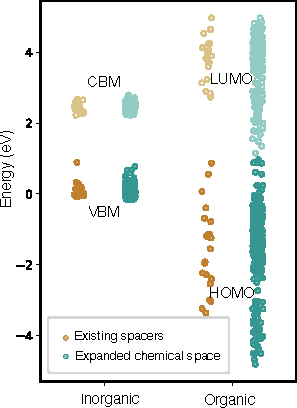
\includegraphics[width=0.5\textwidth]{figures/HT-ML/figure4-5.pdf}
    \caption{Energy level alignment in DJ perovskites with existing spacers and hypothetical organic spacers.}
    \label{fig:figure4.5}
\end{figure}

Our analysis revealed that the majority of DJ perovskites (18 out of 21 experimentally reported structures) exhibit type Ia energy level alignment, characterized by low-energy electrons and holes localized in inorganic layers. The remaining three structures exhibit type IIa alignment. The primary factor dictating this variation in energy level alignment is the frontier molecular orbitals levels of the organic spacers, which exhibit a broad energy variation of $\sim6.1$ eV. In contrast, the inorganic band edges remain relatively invariant, with a variation of only $\sim0.9$ eV (see Figure \ref{fig:figure4.5}). This observation aligns with the common approximation cited in the literature that inorganic energy levels of 2D perovskites can be assumed unchanged with different organic spacers\cite{RN18,RN20}. 

Furthermore, Figure \ref{fig:figure4.5} illustrates how our expanded chemical space exploration has significantly extended the range of organic frontier levels compared to previous studies. The generated DJ perovskites—including $G_0-G_2$ and inverse designed final candidates (introduced later in Chapter \ref{c:result-2})—exhibit an expanded energy distribution of organic frontier levels, covering a much wider range than the reported organic spacers, underscoring the effectiveness of our chemical space exploration approach. 

\subsection{Four factors governing energy level alignment}

\begin{figure}[htbp]
    \centering
    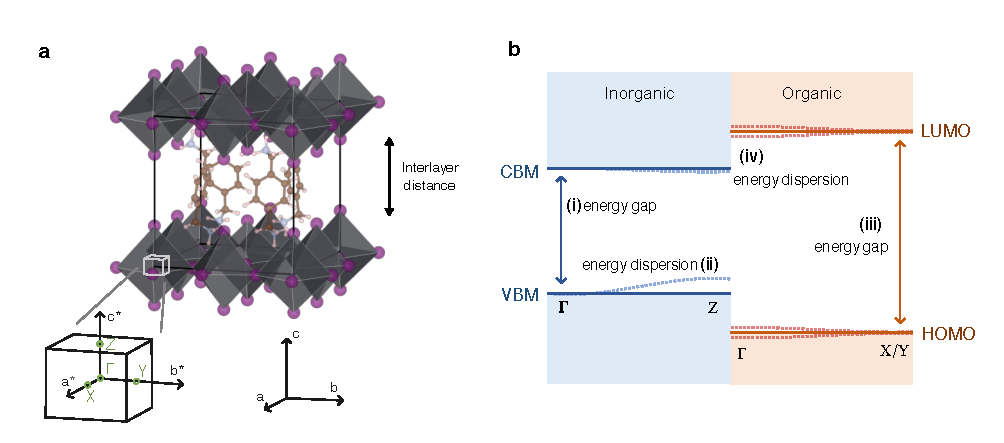
\includegraphics[width=\textwidth]{figures/HT-ML/figure4-6.pdf}
    \caption{Four factors affecting the energy level alignment in DJ perovskites.}
    \label{fig:figure4.6}
\end{figure}

To further understand the structure-property relationships governing energy level alignment in DJ perovskites, we analysed key electronic band structure trends across all structures studied. Four dominant factors were identified, as illustrated in Figure \ref{fig:figure4.6}:

(i) Energy gap at the inorganic band edge ($\Gamma$ point)

(ii) Inorganic band dispersion along the stacking direction ($\Gamma$ to $Z$)

(iii) Energy gap between the organic frontier orbitals (HOMO-LUMO levels)

(iii) Frontier orbital dispersion of the organic spacers

\textbf{Electronic structure of inorganic component}

\begin{figure}[htbp]
    \centering
    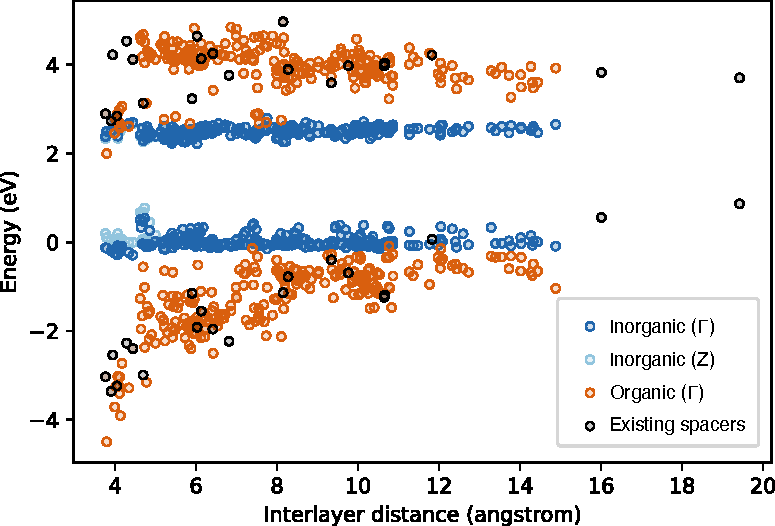
\includegraphics[width=0.9\textwidth]{figures/HT-ML/figure4-7.pdf}
    \caption{Energy level alignment in calculated DJ perovskites plotted against interlayer distance.}
    \label{fig:figure4.7}
\end{figure}

The inorganic layers in DJ perovskites typically form direct bandgap semiconductors with their valence band maximum (VBM) and conduction band minimum (CBM) located at the $\Gamma$ point in the Brillouin zone. However, in cases where interlayer coupling is significant, the bandgap shifts to the Z point. 

The band dispersion is strongly anisotropic, exhibiting strong dispersion in the $\Gamma-X/Y$ direction (in-plane directions in real space), while the dispersion in the $\Gamma-Z$ direction (stacking direction) depends on interlayer interactions. This trend of interlayer interaction is illustrated in Figure \ref{fig:figure4.7}, where the energy level alignment is plotted against the interlayer distance. Interlayer coupling, characterized by the energy difference between the $\Gamma$ and $Z$ point of the inorganic band edge, becomes significant only when the interlayer distance is relatively small.

\begin{figure}[htbp]
    \centering
    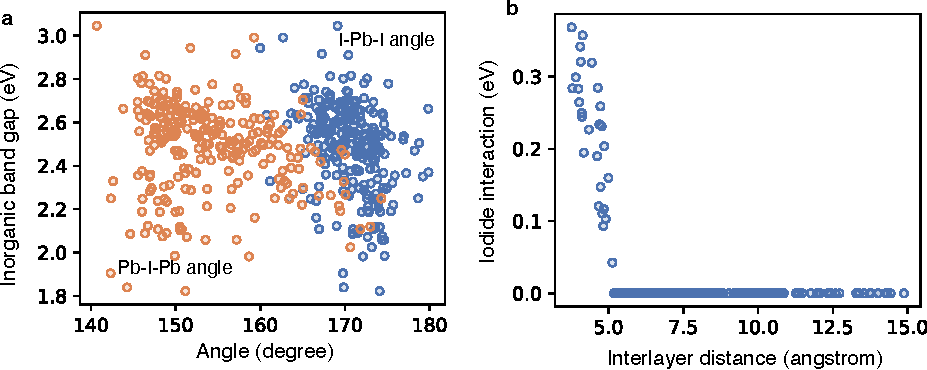
\includegraphics[width=\textwidth]{figures/HT-ML/figure4-8.pdf}
    \caption{Indirect influence of organic spacers on inorganic band edges.}
    \label{fig:figure4.8}
\end{figure}

To further quantify the structure-property relationship between inorganic framework geometry and energy levels, we examined two key structural factors (Figure \ref{fig:figure4.8}):

\begin{itemize}
    \item Factor (i) in Figure \ref{fig:figure4.6} is mainly affected by octahedral tilting and distortion. As shown in Figure \ref{fig:figure4.8}a, variations in the Pb-I-Pb bond angle and I-Pb-I internal distortion significantly impact the inorganic energy gap at the $\Gamma$ point, leading to energy shifts of approximately 1 eV. These distortions arise due to hydrogen bonding interactions between the PbI$_6$ octahedra and the organic cations.
    \item Factor (ii) in Figure \ref{fig:figure4.6} is mainly affected by interlayer distance. As shown in Figure \ref{fig:figure4.8}b, when the interlayer distance decreases below 5.0 $\AA$, iodide-iodide interactions enhance $\Gamma-Z$ energy dispersion, also inducing $\sim$1 eV energy shifts. This behaviour is commonly observed in DJ-phase perovskites with short organic spacers and is consistent with trends reported in ACI-phase perovskites\cite{RN242,RN31}.
\end{itemize}

\textbf{Electronic structure of the organic component}

Unlike the band-like behaviour of the inorganic layers, the organic frontier orbitals (HOMO and LUMO) remain localized and discrete, with minimal dispersion, closely resembling their isolated molecular forms. This occurs because:
\begin{itemize}
    \item There is not interlayer interaction between organic spacers in adjacent layers, resulting in zero dispersion along the $\Gamma-Z$ direction. 
    \item The in-plane ($\Gamma-X/Y$) dispersion is also minimal due to the herringbone packing of organic spacers, which restricts electronic interactions between adjacent organic units. More detailed discussions on the relationship between packing pattern and in-plane dispersion can be found in Chapter \ref{c:method}.
\end{itemize}

\subsection{Simplified modelling of organic frontier levels}

Our analysis confirms that the primary influence of organic spacers on DJ perovskite energy levels lies in their HOMO and LUMO levels, which is primarily a consequence of weak bonding interactions between organic cations and the inorganic framework\cite{RN42,RN144}. 

However, the high computational cost of DFT calculations for large DJ perovskite unit cells limits our ability to simulate thousands of structures. To address this, we propose an efficient approximation: Organic frontier energy levels in hybrid perovskites can be estimated using calculations on isolated cations.

\begin{figure}[htbp]
    \centering
    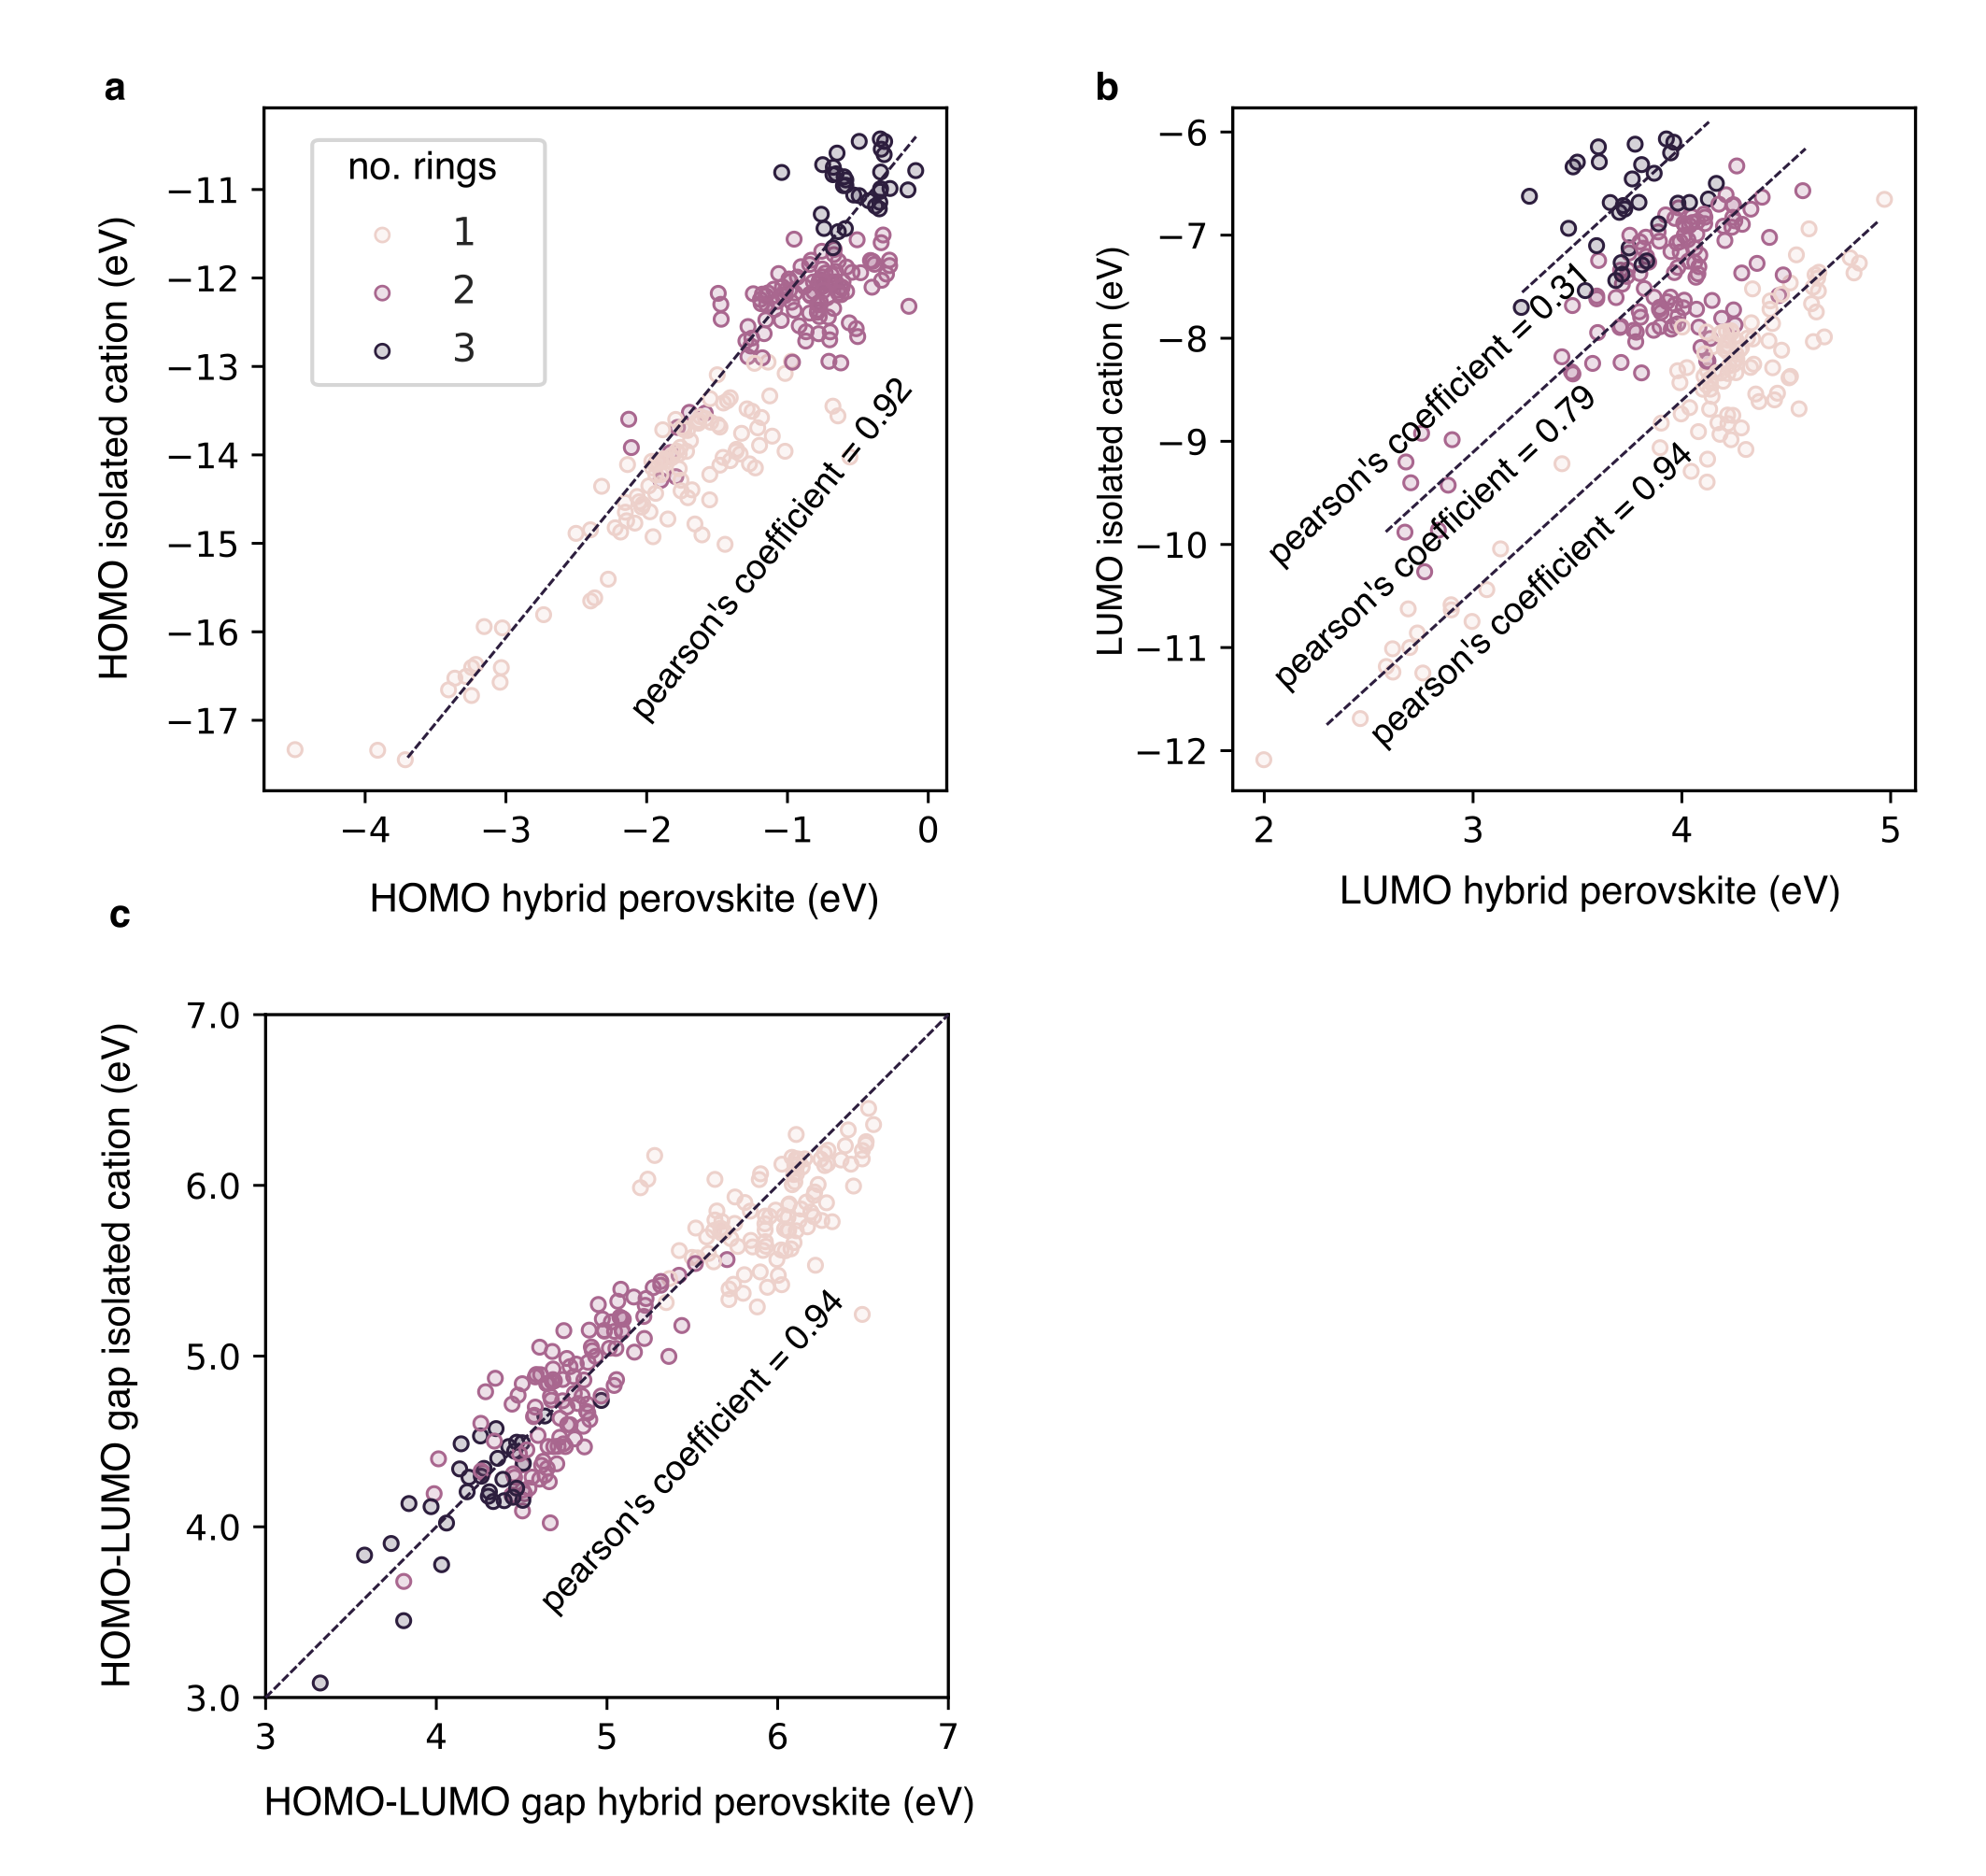
\includegraphics[width=\textwidth]{figures/HT-ML/figure4-9.png}
    \caption{Correlation between organic frontier levels in hybrid perovskites and their isolated molecular forms.}
    \label{fig:figure4.9}
\end{figure}

We computed frontier levels of isolated organic spacers using the B3LYP functional in Gaussian. Figure \ref{fig:figure4.9} compares the frontier orbital energies obtained from hybrid perovskite calculations and isolated organic cations. While absolute energy values differ because of functional choices, basis sets, and the chemical environment, a near-linear relationship emerges between the two calculations:

\begin{itemize}
    \item Figure \ref{fig:figure4.9}a shows that HOMO levels exhibit a linear correlation between hybrid perovskites and their isolated cation counterparts.
    \item Figure \ref{fig:figure4.9}b highlights a similar trend in LUMO levels, with noticeable dependence on the ring count of the organic spacer.
    \item Figure \ref{fig:figure4.9}c indicates that indicates that the HOMO–LUMO gap remains consistent between the two methods.
    
\end{itemize}

By leveraging these correlations, we can predict organic frontier levels without the need for fully relaxed DJ perovskite calculations for each candidate spacer. This significantly reduces the computational cost, enabling us to scale from hundreds to thousands of hypothetical structures—an essential step for generating robust datasets to train machine learning models in the subsequent sections.

\section{Selection and evaluation of machine learning models}\label{section:section4-3}

In the previous sections, we established how organic spacers affect the energy level alignment in DJ perovskites, and we identified key structural descriptors that can serve as input features for predictive modelling. Here, we describe how ML is employed to capture the structure–property relationships between molecular fingerprints and their frontier energy levels, and facilitate the rapid identification of promising spacer candidates.

\subsection{Molecular fingerprint as input feature}

\begin{figure}[htbp]
    \centering
    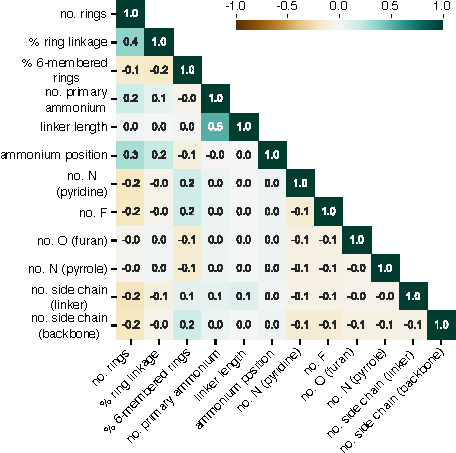
\includegraphics[width=0.9\textwidth]{figures/HT-ML/figure4-10.pdf}
    \caption{Correlation matrix of organic descriptors in the molecular fingerprint.}
    \label{fig:figure4.10}
\end{figure}

To represent each organic spacer, we use a 12-digit molecular fingerprint as the input feature for our machine learning pipeline. This fingerprint does not require additional feature selection, as it was specifically designed to minimize redundancy among descriptors. Indeed, Pearson’s correlation coefficients between fingerprint descriptors are all below 0.5 (see Figure \ref{fig:figure4.10}), confirming low inter-feature correlation and justifying the direct inclusion of all 12 features in model training. This is a significant advantage compared to previous studies that rely on diverse chemical descriptors and require feature selection to reduce multicollinearity\cite{RN315,RN283}.

Our machine learning dataset consists of 3,239 organic spacers spanning generations $G_0-G_3$, with HOMO/LUMO values from high-throughput calculations serving as the target properties. This dataset allows us to explore a broad range of structures and electronic characteristics, setting the stage for robust model training.

\subsection{Comparison of different models}

\begin{figure}[htbp]
    \centering
    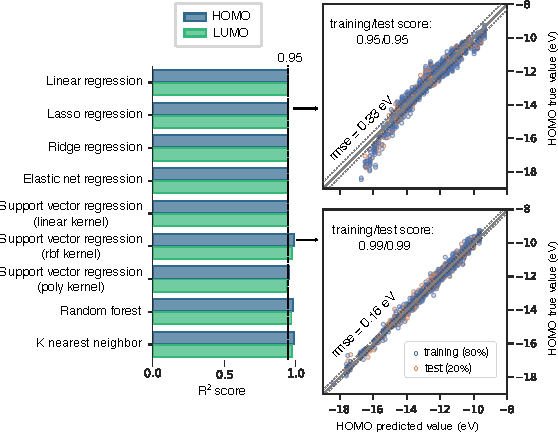
\includegraphics[width=\textwidth]{figures/HT-ML/figure4-11.pdf}
    \caption{Summary of ML model performance for HOMO/LUMO prediction.}
    \label{fig:figure4.11}
\end{figure}

\begin{figure}[htbp]
    \centering
    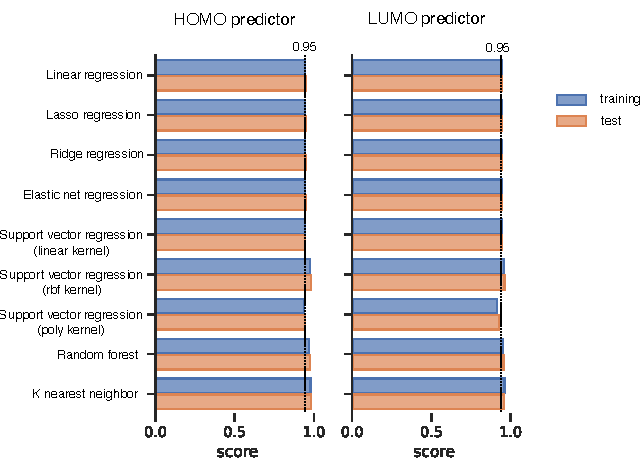
\includegraphics[width=0.9\textwidth]{figures/HT-ML/figure4-12.pdf}
    \caption{Comparison of training/test scores of various ML models for HOMO/LUMO prediction.}
    \label{fig:figure4.12}
\end{figure}

Because our goal is to predict HOMO and LUMO energies from known labels (i.e., computed frontier levels), this is a supervised regression problem. We trained separate machine learning models for HOMO and LUMO predictions respectively, with the dataset split into training and testing sets (80: 20 ratios). All models were evaluated using 15-fold cross-validation to ensure consistent and reliable estimation of fitting error. A variety of linear and non-linear regression methods commonly used in materials science literature were benchmarked, including:
\begin{itemize}
    \item Linear models: linear regression, LASSO regression, Ridge regression, Elastic net regression, Support vector regression with a linear kernel.

    \item Non-linear models: Random Forest, K nearest neighbour, Support Vector Regression with radial basis function (rbf) kernel or polynomial kernel. 
\end{itemize}

Figure \ref{fig:figure4.11} summarizes the R$^2$ scores (ranging from 0 to 1, with higher values indicating better predictions) for each model. Across both HOMO and LUMO predictions, nonlinear models achieve slightly higher R$^2$ scores (around 0.99/0.97) than linear models (around 0.95/0.95). Notably, no overfitting was detected, as evidenced by comparable performance on both training and test sets (Figure \ref{fig:figure4.12}).

Despite their slightly lower performance for low-energy frontier levels, linear models capture the overall trend effectively. This difference becomes clearer in Figure \ref{fig:figure4.13} (HOMO) and Figure \ref{fig:figure4.14} (LUMO), which plot predicted vs. true energy values alongside model scores and root mean squared errors (RMSE). While nonlinear models better capture the extreme regions of energy, linear models show no significant deviations from the overall relationship.

Since our primary objective was to classify energy level alignment types (e.g., Type Ia, Type IIa, etc.) rather than predict absolute HOMO/LUMO values, a slight accuracy gap at the extremes is not critical. By optimizing the decision boundary, linear models can serve as a highly interpretable alternative without a significant loss in performance. Consequently, linear models are chosen for subsequent analysis and feature interpretation.

\begin{figure}[htbp]
    \centering
    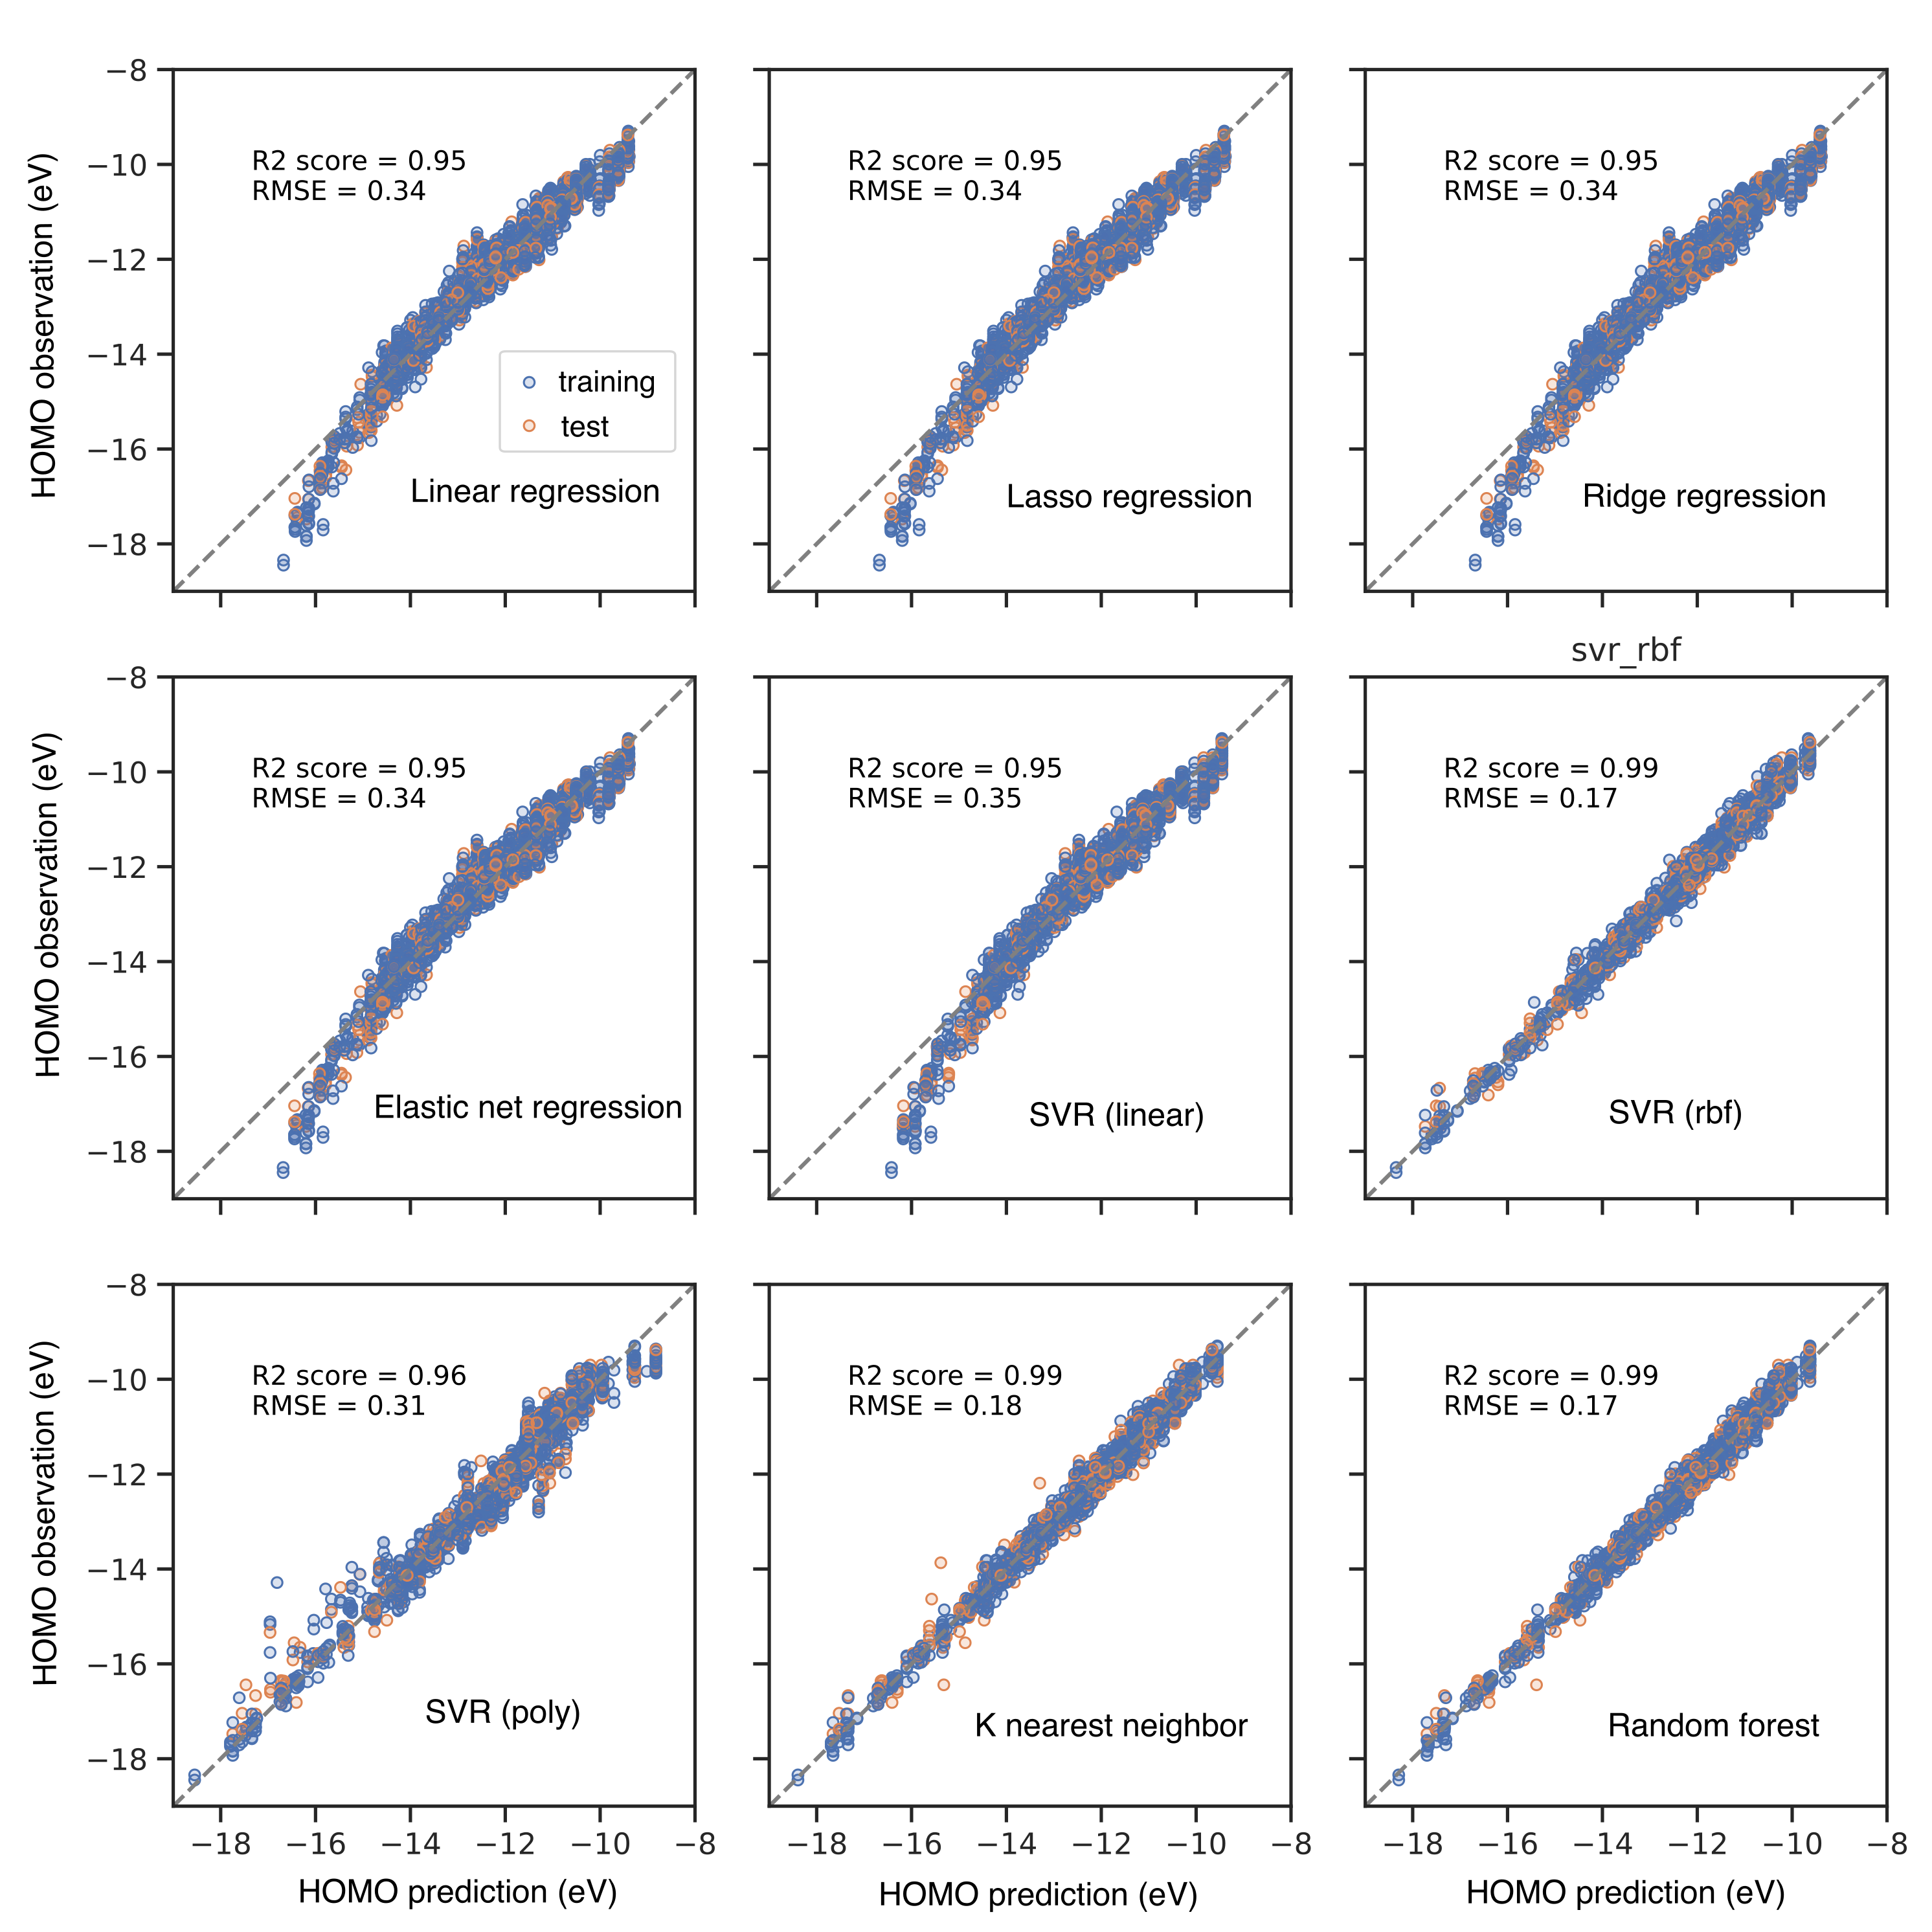
\includegraphics[width=\textwidth]{figures/HT-ML/figure4-13.png}
    \caption{Predicted vs. true values for HOMO level across various ML models.}
    \label{fig:figure4.13}
\end{figure}

\begin{figure}[htbp]
    \centering
    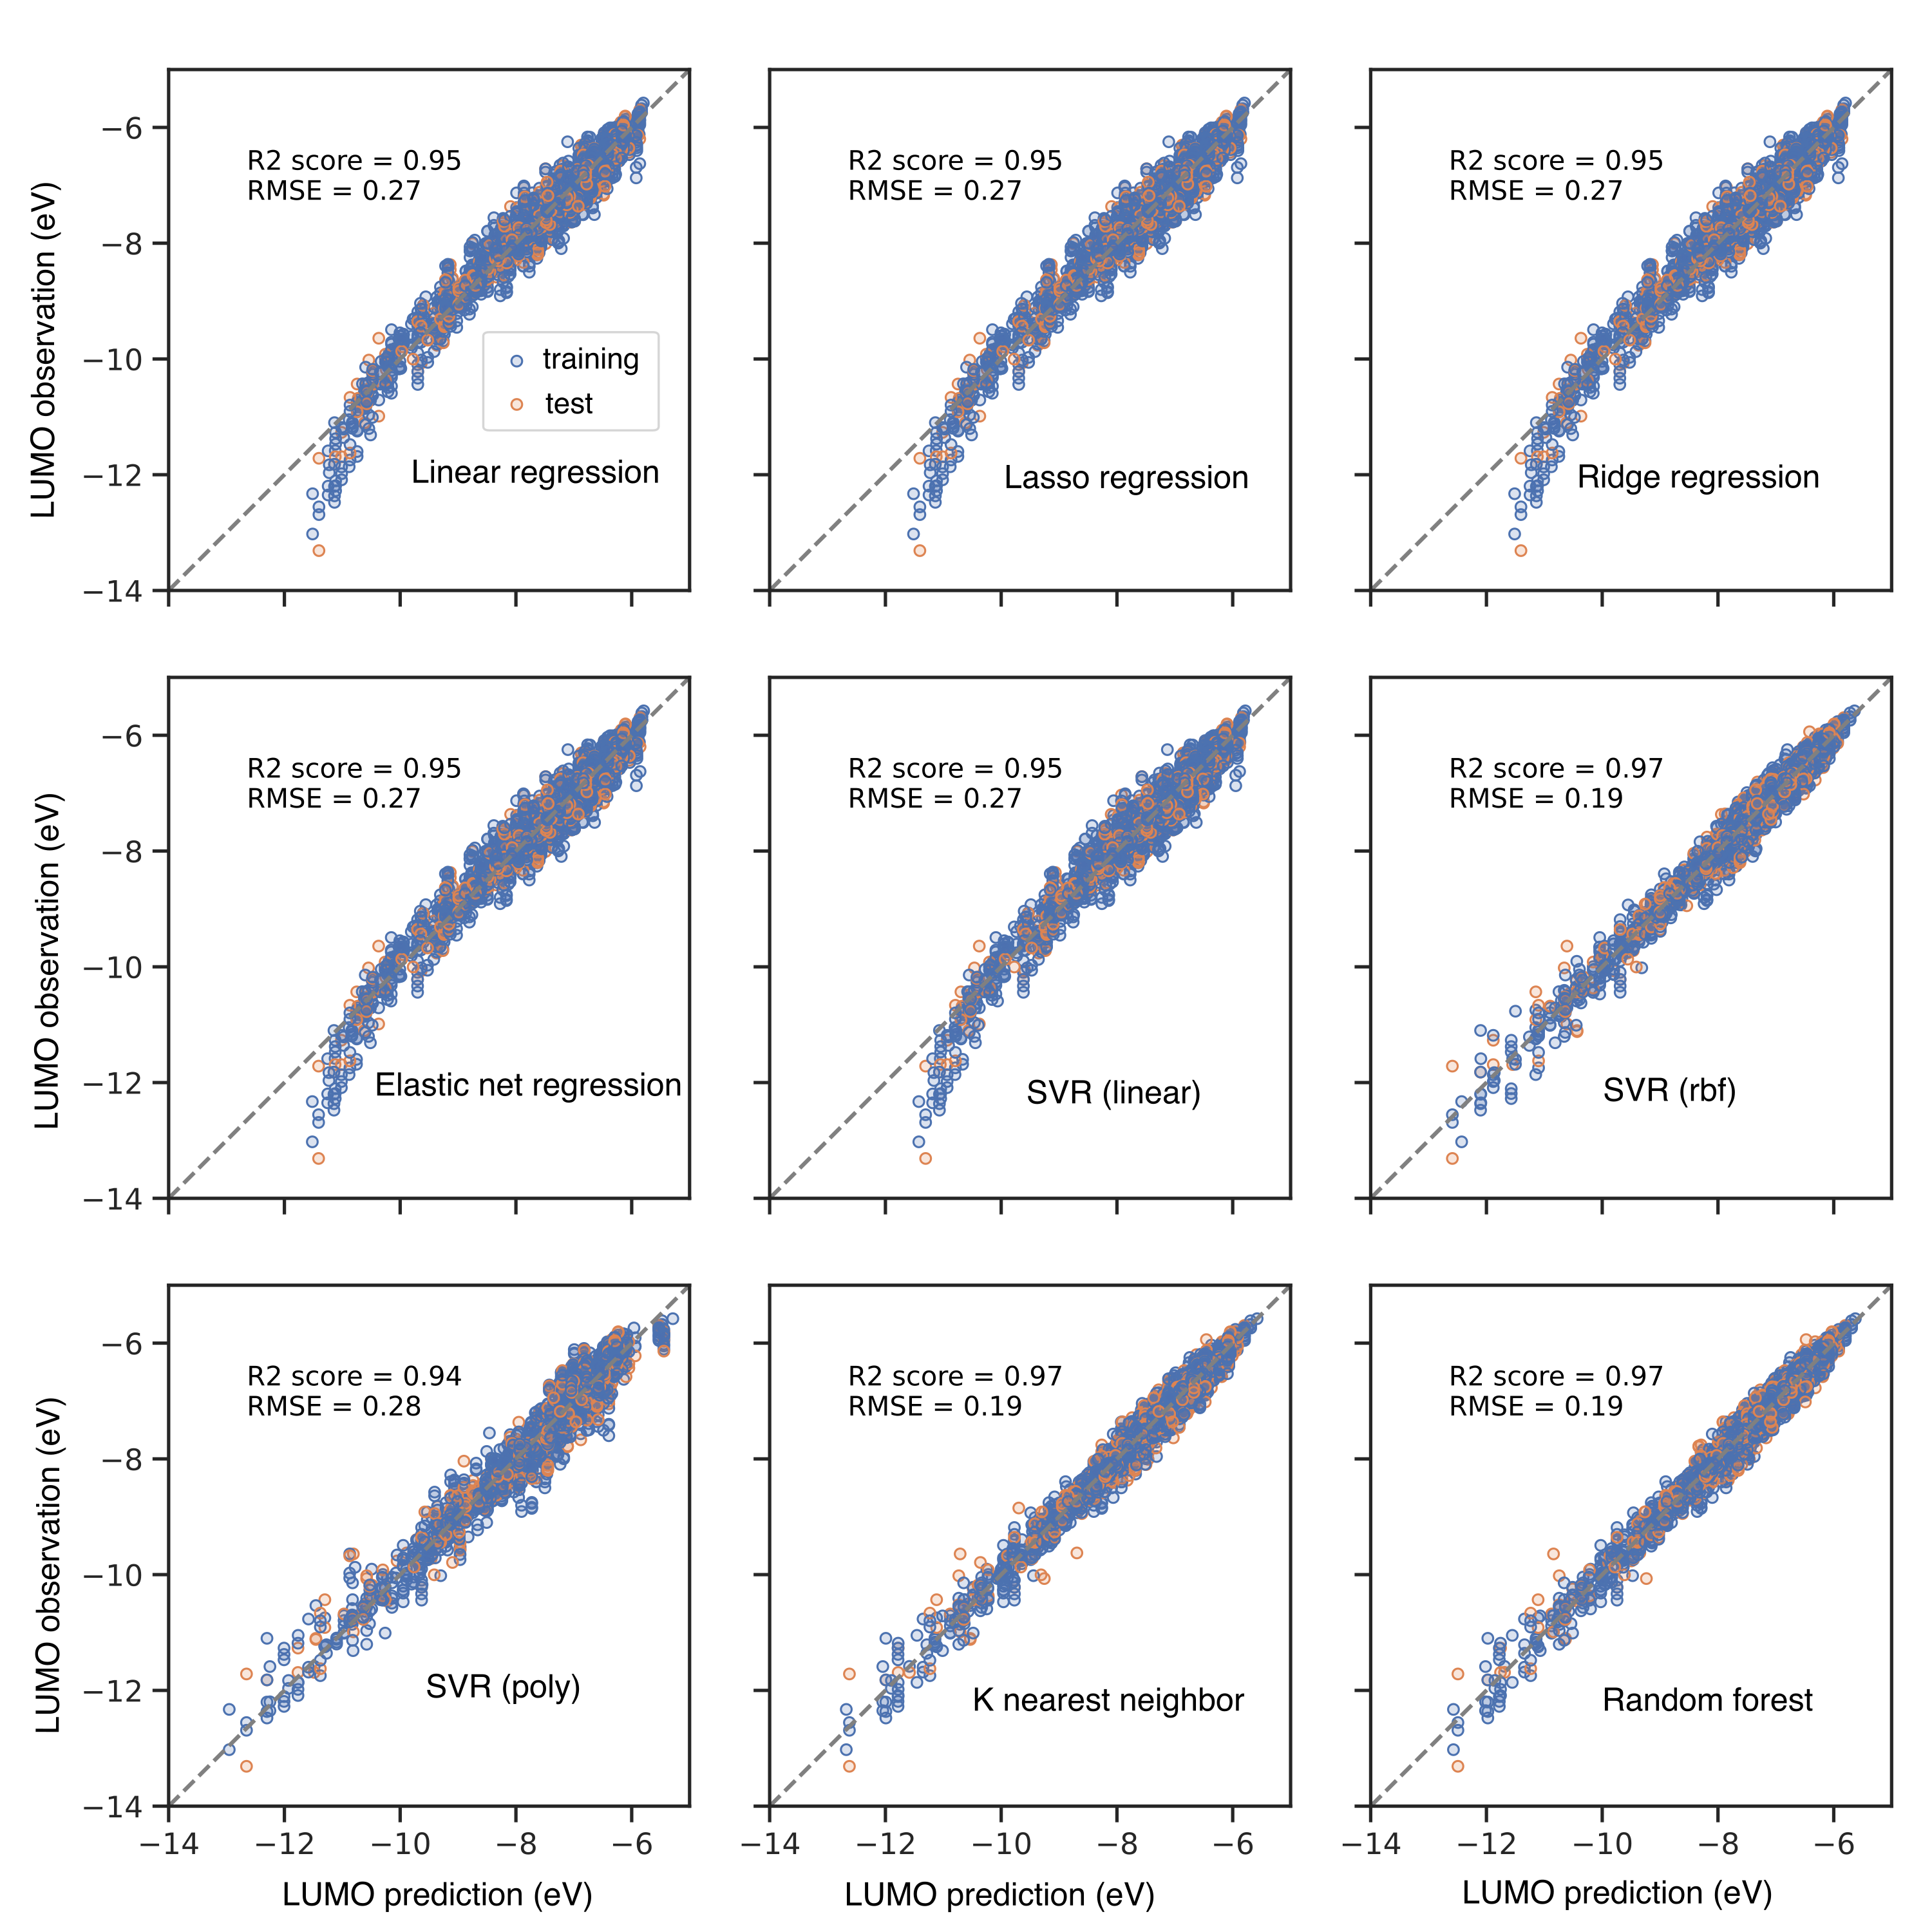
\includegraphics[width=\textwidth]{figures/HT-ML/figure4-14.png}
    \caption{Predicted vs. true values for LUMO level across various ML models.}
    \label{fig:figure4.14}
\end{figure}

\section{Interpretation of structure-property relationships}\label{section:section4-4}

In this section, we explore various approaches to interpreting the machine learning model. We demonstrate how different model interpretation methods can yield slightly different feature importance rankings while still preserving the same underlying physical meaning.

\subsection{Feature coefficient}

In many traditional machine learning approaches—especially linear models—the model parameters (often referred to as coefficients or weights) provide a direct way to interpret how each input feature influences the predicted outcome. In our case, these coefficients offer insight into how various organic descriptors (encoded in the 12-digit fingerprint) affect the HOMO/LUMO energy levels of the organic spacers.

Since our data undergo feature normalization (standardization) before training, two types of coefficients are relevant: normalized feature coefficient (directly reported by the trained model), and unnormalized feature coefficient (raw coefficient rescaled to the original units).

\textbf{Normalized feature coefficient}

During model training, each descriptor is standardized by subtracting its mean and dividing by its standard deviation. As a result, the coefficients reported by the model reflect the effect of a one-standard-deviation change in a descriptor on the predicted HOMO or LUMO. Larger absolute coefficients indicate greater importance, while the sign (positive/negative) denotes whether the feature increases or decreases the predicted value.

\begin{figure}[htbp]
    \centering
    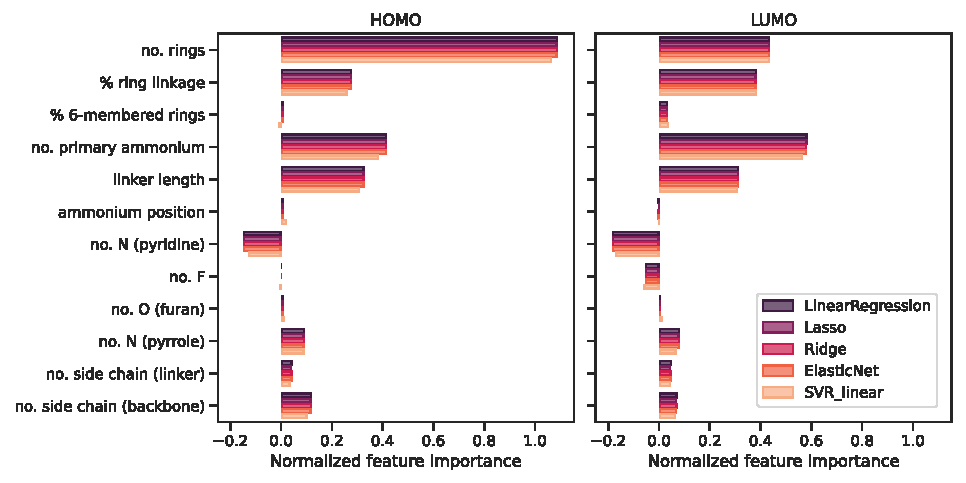
\includegraphics[width=\textwidth]{figures/HT-ML/figure4-15.pdf}
    \caption{Normalized feature coefficients of linear ML models used in this work.}
    \label{fig:figure4.15}
\end{figure}

Figure \ref{fig:figure4.15} compares the normalized feature coefficients from various linear models—including Linear Regression, LASSO, Ridge, Elastic Net, and Linear SVR. All models yield similar coefficients, suggesting that regularization (L1, L2, or a combination) does not drastically alter the identification of the most influential features. Moreover, the consistency in coefficients across models indicates minimal overfitting.

In general, features related to the conjugated backbone (e.g., no. rings) and tethering ammonium groups (e.g., no. primary ammonium) strongly influence both HOMO and LUMO predictions. Notably, most features affect HOMO and LUMO in a comparable manner, implying that variations in the HOMO–LUMO gap primarily arise from a few key descriptors. For HOMO, all features except “no. pyridine-type nitrogens” contribute positively, with number of rings exerting the largest effect. For LUMO, pyridine-type nitrogen and fluorine substitution exert negative contributions, whereas number of rings plays a slightly smaller role compared to HOMO.

Given its L1 regularization, LASSO provides a convenient means of highlighting key features by favouring sparse solutions. Therefore, LASSO regression serves as our representative linear model for subsequent interpretation and prediction, although the insights remain applicable to all linear models.

\textbf{Unnormalized feature coefficient}

While normalized coefficients gauge the effect of a one-standard-deviation change, the unnormalized coefficients express how a one-unit increase in each descriptor affects the HOMO or LUMO in real (eV) units. Consequently, unnormalized coefficients are often more intuitive in a materials science context, where absolute energy shifts matter.

As an example, the LASSO-based HOMO predictor can be written as:

\begin{equation}
\begin{split}
    HOMO &= 1.33\,x_1 + 0.61\,x_2 + 0.05\,x_3 + 1.33\,x_4 + 0.52\,x_5 + 0.18\,x_6 - 0.30\,x_7 + 0.00\,x_8 \\
         &\quad + 0.06\,x_9 + 0.44\,x_{10} + 0.11\,x_{11} + 0.24\,x_{12} - 19.25
\end{split}
\end{equation}


Here, $x_1…x_{12}$ represent the 12 molecular descriptors, and the coefficients specify how changes in each descriptor shift the predicted HOMO (in eV). Notably, $x_1$ and $x_4$—which corresponded to no. rings and no. primary ammonium groups—dominate, indicating their strong contribution to the HOMO level.

\begin{figure}[htbp]
    \centering
    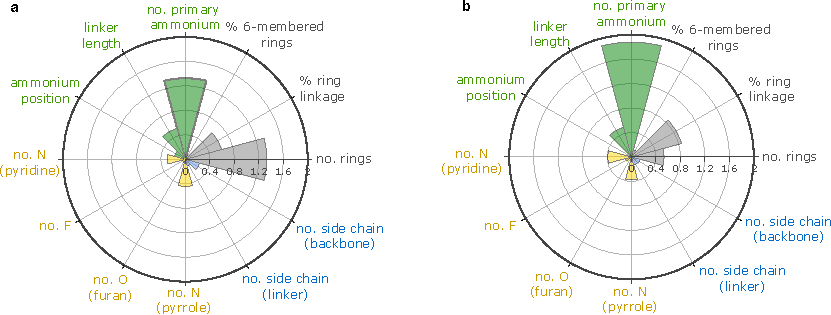
\includegraphics[width=\textwidth]{figures/HT-ML/figure4-16.pdf}
    \caption{Unnormalized feature coefficients (absolute value) from Lasso regression model. }
    \label{fig:figure4.16}
\end{figure}

A similar expression applies to LUMO, and Figure \ref{fig:figure4.16} visualizes the absolute values of the unnormalized coefficient for both HOMO and LUMO in radar plot. Overall, normalized and unnormalized coefficients are consistent; however, descriptors with broader numerical ranges (e.g., number of rings, which varies from 1 to 4) show relatively smaller unnormalized coefficients, whereas features with narrow ranges (e.g., number of primary ammonium groups, which varies from 1 to 2) appear more prominent.

Despite these differences, the physical insights remain the same: conjugation (number of rings) and tethering ammonium groups play crucial roles in frontier orbital energies. The next subsection delves into a comprehensive interpretation of how each feature influences HOMO/LUMO levels.

\subsection{SHAP value analysis}

SHAP (SHapley Additive exPlanations) is a popular method for explaining the output of complex machine learning models. At its core, SHAP leverages concepts from cooperative game theory—specifically Shapley values—to attribute the contribution of each feature to a model’s prediction. To further interpret how individual features influence predictions, we employ SHAP analysis, which assigns each descriptor a contribution (positive or negative) to the final HOMO or LUMO prediction. 

Instead of using the average predicted value (the default SHAP baseline), we use the predicted value of $G_0$ molecule, PDMA, as reference molecule. This makes the SHAP values more physically meaningful because each feature’s contribution is interpreted relative to the G0 molecule rather than to a broad average. Concretely, for each data sample, our model produces 12 SHAP values (one per feature). Summing all 12 SHAP values plus the baseline prediction (the prediction for $G_0$) typically yields the model’s actual prediction for that sample.

\textbf{Global feature importance}

\begin{figure}[htbp]
    \centering
    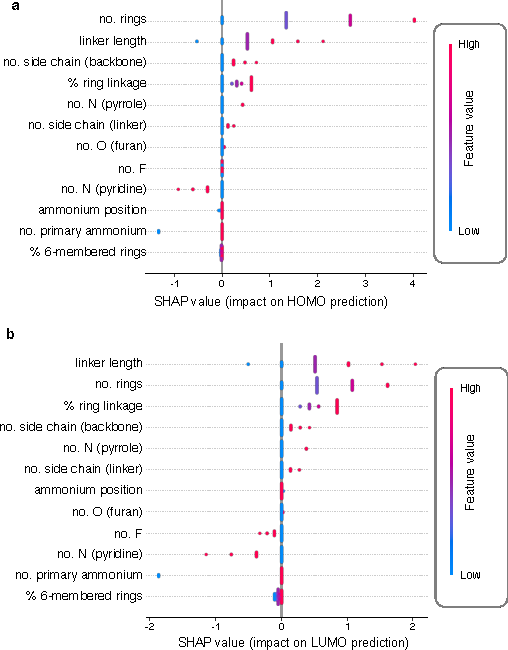
\includegraphics[width=0.8\textwidth]{figures/HT-ML/figure4-17.pdf}
    \caption{SHAP value analysis of HOMO and LUMO predictor.}
    \label{fig:figure4.17}
\end{figure}

Figure \ref{fig:figure4.17} shows a SHAP summary plot (i.e., beeswarm plot), which provides a global view of feature importance and how each feature’s impact varies across samples. The 12 features appear on the y-axis in order of their overall influence, with the most impactful features at the top. Each dot in a row represents a SHAP value for one data point, and the x-axis indicates the magnitude and direction of the feature’s contribution (left for a negative shift from $G_0$, right for a positive shift). Because most features (e.g., no. rings) take discrete values, their SHAP values often cluster in distinct groups rather than forming a continuous distribution. A wider spread of SHAP values in a feature’s row means that feature has a more variable effect across different molecules. For example, “number of rings” can shift the predicted HOMO by as much as 4 eV relative to $G_0$.

The summary plot highlights the influence of key features. Consistent with our analysis of feature coefficient in previous subsection, the features related to the conjugated backbone and tethering ammonium groups being the most significant. Among these, the number of aromatic rings in the conjugated backbone emerges as a critical factor, directly influencing the degree of conjugation—a well-established design rule in organic semiconductors\cite{RN282} that has also found application in 2D perovskites\cite{RN18,RN20}. In addition to conjugation, the analysis underscores the significance of electron richness, another foundational principle in the design of organic semiconductors\cite{RN282}. For tethering ammonium groups, the electron-rich alkyl groups associated with primary ammonium can raise the frontier levels by increasing the linker length or the number of primary ammonium groups. The effect of heteroatom substitution varies depending on the electronic nature of the substituent. For example, pyridine-type nitrogen, being electron-withdrawing, lowers both HOMO and LUMO, while pyrrole-type nitrogen, being electron-donating, raises both levels. Interestingly, fluorination—widely used to enhance stability in 2D perovskite spacers due to the large dipole moment induced by its electron-withdrawing ability\cite{RN84,RN392}—showed a relatively minor influence on the frontier levels in this study. This limited effect may stem from fluorine substitution not directly participating in the conjugated $\pi$-system. While highly electronegative, fluorine’s influence remains localized, resulting in minimal perturbation to the frontier orbitals. 

Compared to feature coefficient discussed in previous section, the linker length emerges as the most influential factor in LUMO prediction. This is because all the data is calibrated by baseline value of $G_0$ molecules, instead of the mean value. This shows that change in linker length can produce the largest deviation from LUMO of $G_0$ molecule.

\textbf{Individual feature importance of representative molecule}

After examining the global summary, we now present visualizations of SHAP values for individual samples. This is achieved using waterfall plots, which decompose a single prediction into its component feature contributions, illustrating how each feature influences the model’s output above or below the baseline (which, in this case, is the $G_0$ molecule). Two categories of organic spacers are analyzed below, molecules with relatively high HOMO, and molecules with relatively low LUMO.

\begin{figure}[htbp]
    \centering
    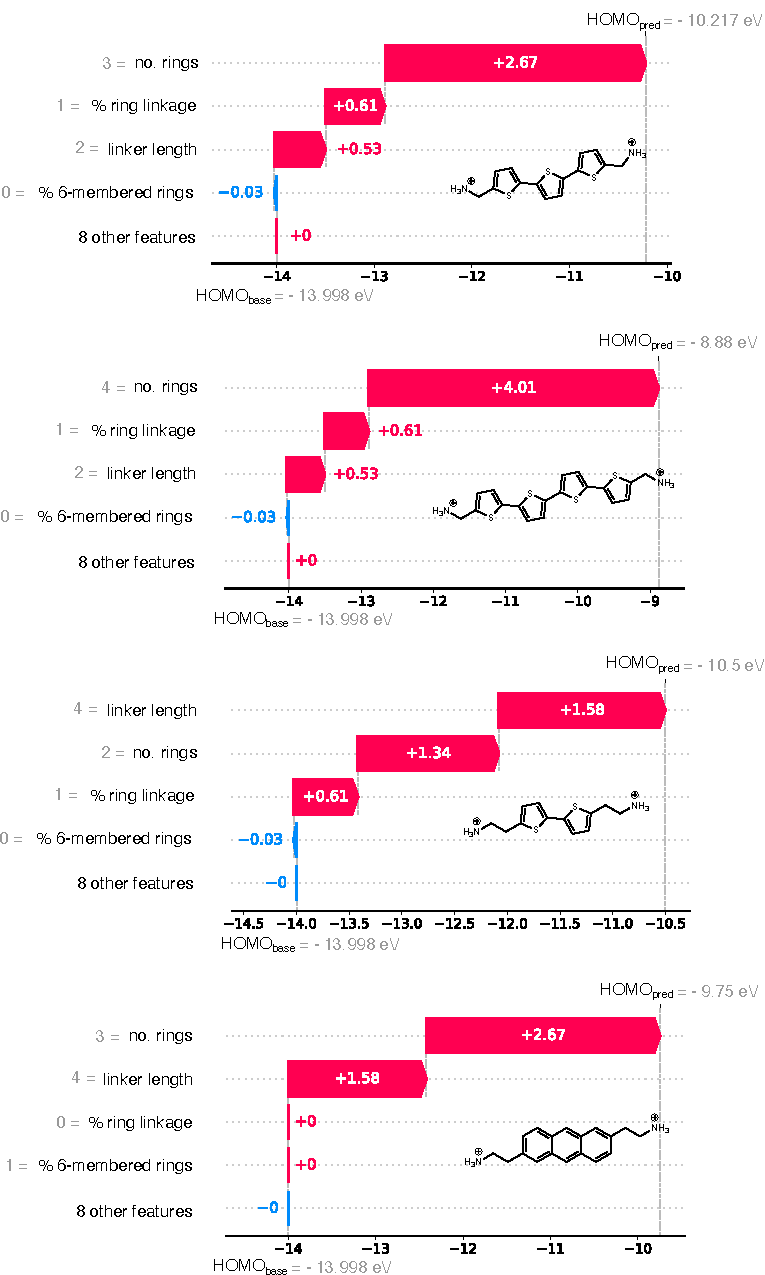
\includegraphics[width=0.8\textwidth]{figures/HT-ML/figure4-18.pdf}
    \caption{SHAP value analysis of representative organic spacers in type IIa.}
    \label{fig:figure4.18}
\end{figure}

Figure \ref{fig:figure4.18} presents SHAP value analysis for four organic spacers with relatively high HOMO levels, which are later validated to achieve Type IIa alignment. The SHAP values are calibrated using the $G_0$ molecule as a baseline (horizontal axis on the left, where HOMO = -13.998 eV). Each feature’s SHAP value is represented by a bar extending to the right (positive contribution, colored in pink) or to the left (negative contribution, colored in blue). The bars are arranged in order of their magnitude of impact, allowing for a visual step-by-step decomposition from the baseline to the final predicted value.

The primary driving factors for a higher HOMO level vary across molecules. For instance, in the first molecule, the most significant contributor is the number of rings, followed by the percentage of ring linkage. In the third molecule, the linker length is the dominant feature, followed by the number of rings.
    
\begin{figure}[htbp]
    \centering
    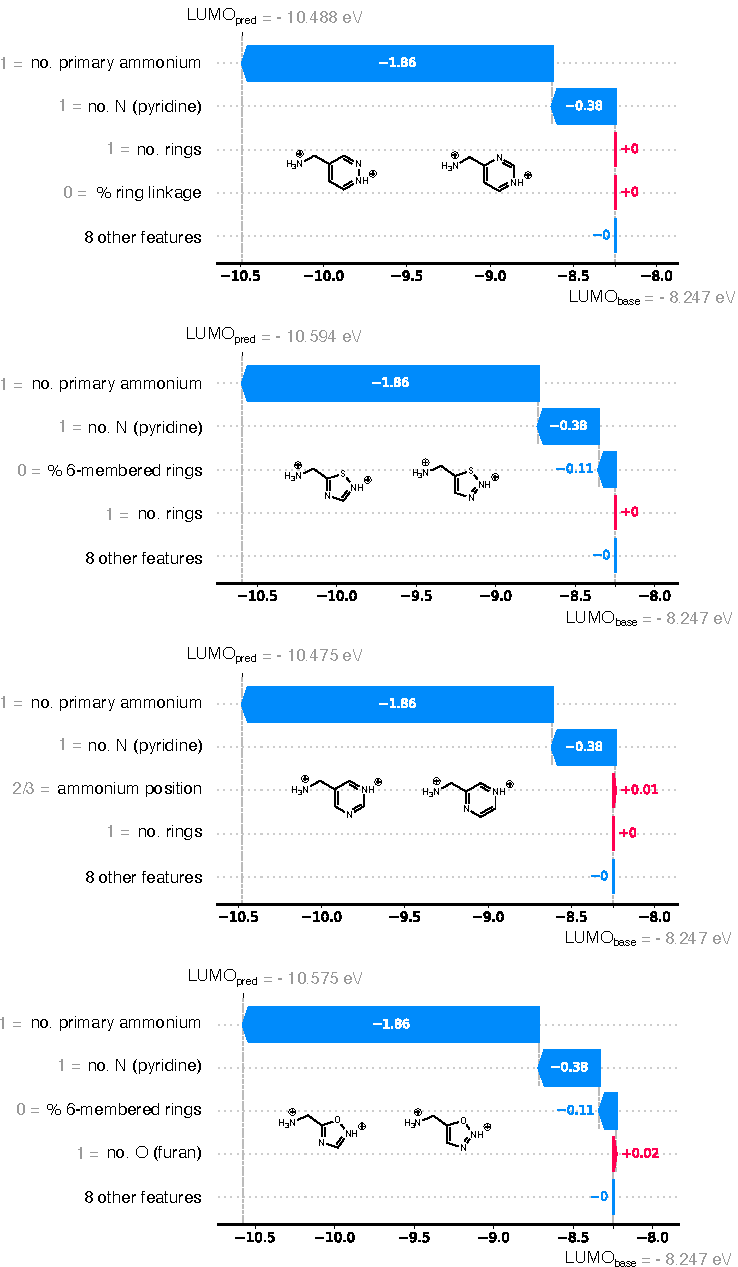
\includegraphics[width=0.8\textwidth]{figures/HT-ML/figure4-19.pdf}
    \caption{SHAP value analysis of representative organic spacers in type IIb.}
    \label{fig:figure4.19}
\end{figure}

Figure \ref{fig:figure4.19} illustrates the SHAP analysis of eight organic spacers predicted to achieve Type IIb alignment, characterized by relatively low LUMO levels.

The results indicate that the most significant factor driving a lower LUMO level across these molecules is the reduction in the number of primary ammonium groups.

These findings demonstrate the predictive capability of the interpretable machine learning model, which allows for the estimation of organic frontier energy levels—and by extension, the energy level alignment of DJ perovskites—for any organic spacer given its fingerprint representation. This capability accelerates the discovery process by enabling the rapid identification of promising candidates with targeted energy level alignment types.

\section{Chapter summary}

This chapter presented a combined high-throughput DFT and machine learning workflow for exploring the chemical space of organic spacers in 2D perovskites. We first generated a diverse library of hypothetical organic cations through systematic morphing operations. High-throughput DFT calculations were then performed to evaluate key physical properties across this expanded chemical space. Machine learning models were trained and benchmarked, achieving high predictive accuracy. Importantly, these models enabled rapid property prediction for large molecular sets and revealed meaningful structure–property relationships. The outcomes from this chapter establish a robust foundation for the inverse design and screening of novel spacer candidates in the following chapters.



    \chapter[Synthesis Feasibility Screening and Final Candidate Validation]{Synthesis Feasibility Screening and Final Candidate Validation}\label{c:result-2}

One of the fundamental challenges in AI-assisted materials discovery is ensuring that computationally predicted materials are experimentally realizable. Section \ref{section:section5-1} introduces a two-step screening approach designed to evaluate the practical synthesis feasibility of 2D perovskites. Sections \ref{section:section5-2} present the inverse design of final candidates, integrating both targeted energy level alignment and synthesis feasibility constraints to identify experimentally viable DJ-phase perovskites.

\section{Synthesis feasibility screening}\label{section:section5-1}

\subsection{Rationale and challenges}
Synthesis feasibility is a key bottleneck in AI-assisted materials discovery, acting as the bridge between theoretical predictions and experimental realization\cite{RN409,RN521}. While previous studies have investigated the synthetic feasibility of RP perovskites\cite{RN315,RN283}, no systematic approaches have been applied to DJ perovskites. This lack of established protocols arises due to two main challenges:

\begin{enumerate}
    \item Limited exploration of diammonium spacers: Unlike RP perovskites, which utilize a wide range of monoammonium cations, DJ perovskites require diammonium cations, whose synthetic pathways remain relatively underexplored.
    \item Scarcity of negative data: The absence of well-documented failed synthesis attempts (e.g., cases forming 1D or 0D phases instead of 2D structures) makes it difficult to train predictive models using traditional machine learning approaches\cite{RN422,RN592}. 
\end{enumerate}

\begin{figure}[htbp]
    \centering
    \includegraphics[width=\textwidth]{figures/synthesis-feasibility/figure5-1.png}
    \caption{Summary of synthesis feasibility screening result.}
    \label{fig:figure5.1}
\end{figure}

To address this challenge, we developed a two-step computational screening approach, mimicking the experimentalist’s approach to 2D perovskite synthesis: 

Step 1: Synthetic accessibility of organic spacers—determines whether the generated organic spacers are practically synthesizable using established chemical routes.

Step 2: Formability of 2D DJ perovskite structures—evaluate whether a given organic spacer is likely to form a stable 2D DJ perovskite phase rather than collapsing into 1D or 0D structures.

This workflow is illustrated in Figure \ref{fig:figure5.1}, with screening results shown for generations $G_0-G_4$. The following subsections provide detailed analyses of each screening step.

\subsection{Step 1: Synthetic accessibility of organic spacers}

\textbf{Using PubChem as a proxy for practical synthesizability}

\begin{figure}[htbp]
    \centering
    \includegraphics[width=0.7\textwidth]{figures/synthesis-feasibility/figure5-2.png}
    \caption{Number of generated organic spacers vs. existing spacers in G0-G4.}
    \label{fig:figure5.2}
\end{figure}

Rather than calculating a theoretical synthesis feasibility score, which is common in organic chemistry, we use PubChem presence as a proxy for practical synthesizability. This approach is well-established in 2D perovskite literature\cite{RN315}, as molecules listed in PubChem are generally commercially available or synthetically documented.

In our expanded chemical space ($G_0$-$G_4$), we find that 4.9\% of generated spacers are present in PubChem. The fraction of synthesizable molecules decreases progressively from $G_0$ to $G_4$ (Figure \ref{fig:figure5.2}), reflecting the increasing structural complexity of higher-generation molecules. This trend is expected since earlier generation spacers are structurally simpler and more likely to resemble known compounds, while higher-generation spacers, derived through iterative molecular morphing, tend to be chemically novel.



\textbf{Synthetic accessibility across energy level alignment types}

To determine whether synthesis feasibility is correlated with the energy level alignment type, we analysed the PubChem presence of spacers in $G_0-G_4$ with different ML-predicted energy level alignments:
\begin{itemize}
    \item Type Ib spacers present the greatest synthetic challenges, as none of them are found in PubChem.
    \item Type IIa spacers are also rare, with only 0.1\% appearing in PubChem. 
    \item Type IIb spacers are the most readily accessible, with 17.5\% present in PubChem. 
\end{itemize}

These findings suggest that certain energy alignment types are inherently more difficult to synthesize, posing additional challenges in the inverse design process.

\textbf{Structural factors affecting synthetic accessibility}

\begin{figure}[htbp]
    \centering
    \includegraphics[width=\textwidth]{figures/synthesis-feasibility/figure5-3.pdf}
    \caption{Logistic regression analysis of the relationship between fingerprints and PubChem existence.}
    \label{fig:figure5.3}
\end{figure}

To further understand why certain molecular structures are more synthetically accessible, we trained a classification model to predict whether a given organic spacer appears in PubChem. This model follows a logistic regression framework, where:

\begin{itemize}
    \item Input Features: Molecular fingerprint descriptors.
    \item Target Property: Binary classification (exists in PubChem = 1, not in PubChem = 0).
\end{itemize}

We present the key performance metrics of the logistic regression model in Figure \ref{fig:figure5.3}. The confusion matrix (Figure \ref{fig:figure5.3}a) compares the model’s predictions with the actual labels, showing an overall accuracy of 93\%, meaning that 93\% of the total predictions were correct.

To further evaluate the model’s discriminative ability, we examine the Receiver Operating Characteristic (ROC) curve (Figure \ref{fig:figure5.3}b) and its corresponding Area Under the Curve (AUC) score. In general, a model with no discriminative power (random guessing) produces a diagonal ROC curve from (0,0) to (1,1), with an AUC of 0.5. In contrast, a perfect classifier would have a curve that rises sharply to (0,1) and extends to (1,1), corresponding to an AUC of 1.0.
Our model achieves an AUC of 0.96, with the ROC curve closely approaching the top-left corner, indicating strong predictive performance and a high degree of reliability in capturing the relationship between molecular fingerprints and synthesis feasibility.



Using SHAP value analysis, we identified key molecular features that influence synthetic accessibility (Figure \ref{fig:figure5.3}c).
The most significant descriptors include:

\begin{itemize}
    \item Number of aromatic rings: Molecules with more rings are generally less likely to be found in PubChem;
    \item Side-chain modifications: Certain branched or bulky substituents reduce synthetic accessibility;
    \item Heteroatom substitutions, especially fluorination and pyridine type nitrogen negatively impact synthesizability.
    
\end{itemize}

These findings suggest that molecular complexity—particularly higher ring counts, side chains and heteroatom substitution—tends to reduce synthetic feasibility. This aligns with general organic synthesis trends, where molecules with multiple fused rings and electronegative substitutions are often more difficult to synthesize.

By integrating PubChem data into our feasibility screening, we ensure that our selected candidates remain practically synthesizable. Although most of the identified $G_0-G_4$ spacers have not yet been explored for 2D perovskites, their presence in PubChem suggests that their chemical synthesis pathways are well established, making them promising candidates for experimental validation.

\subsection{Step 2: 2D structure formability analysis}

Following the synthetic accessibility screening, the next step evaluates the formability of 2D DJ perovskite structures. A key determinant of perovskite formability is the hydrogen-bonding interaction between the organic spacer and the inorganic framework. It has been established in the field of 2D perovskite that hydrogen bonding plays a crucial role in stabilizing 2D perovskite structures.

\textbf{Hydrogen bonding as a formability criterion}

To establish hydrogen bonding potential, we examine the interaction between donor and acceptor atoms. For a hydrogen bond to form, two conditions must be met:
\begin{enumerate}
    \item A hydrogen donor atom – A hydrogen atom covalently bonded to an electronegative element (e.g., nitrogen in ammonium groups).
    \item A hydrogen acceptor atom – A highly electronegative element, capable of accepting a hydrogen bond (e.g., halide anions (I⁻, Br⁻, Cl⁻) in the perovskite framework).
\end{enumerate}

In 2D perovskites, the halide atoms in the inorganic layers serve as hydrogen acceptors, while hydrogen-donor groups originate from the organic spacers, typically from nitrogen atom. However, not all nitrogen atoms in organic spacers are capable of forming hydrogen bonds.


\begin{figure}[htbp]
    \centering
    \includegraphics[width=\textwidth]{figures/synthesis-feasibility/figure5-4.pdf}
    \caption{Hydrogen-donor nitrogen for hydrogen bond formation in 2D perovskite.}
    \label{fig:figure5.4}
\end{figure}

Figure \ref{fig:figure5.4} categorizes the four nitrogen types present in the organic spacers examined in this study. Among these, only three can act as hydrogen donors:

(1) Primary ammonium ($-$NH$_3$$^+$)

(2) Protonated pyridine-type nitrogen ($-$NH$^+-$)

(3) Pyrrole-type nitrogen ($-$NH$-$)

Conversely, unprotonated pyridine-type nitrogen ($-$N$-$) cannot serve as a hydrogen donor, as it lacks a covalently bonded hydrogen. 

A few representative organic spacers containing these nitrogen types are illustrated in Figure \ref{fig:figure5.4}. For instance, in the last example, the molecule contains two pyridine-type nitrogen atoms. In its neutral form, both nitrogen atoms are equivalent, with no hydrogen bonding capability due to the absence of a covalently bonded hydrogen. However, in its charged form, if one of the nitrogen atoms becomes protonated, the additional hydrogen enables hydrogen bond formation with the inorganic framework, thereby influencing 2D structure formability.

To ensure accurate descriptor selection, our formability analysis exclusively considers hydrogen-donor nitrogen atoms while excluding non-donor types (e.g., unprotonated pyridine-type nitrogen).

\textbf{Formability descriptors}

The ability of a hydrogen-donor nitrogen to form a hydrogen bond depends not only on its presence but also on whether it can reach the inorganic framework’s halide atoms. This interaction is influenced by the topological and steric properties of the organic spacer.
To quantify these effects, we adopt four key formability descriptors, previously established in RP perovskite formability studies\cite{RN315,RN12}.

\begin{itemize}
    \item steric hindrance index (STEI) – measures spatial constraints around the hydrogen donor.
    \item eccentricity – evaluates molecular shape (ratio between height and width)
    \item nitrogen-nitrogen pair distance (Dis$_{NN}$)—Assess the spatial separation of tethering ammonium groups.
    \item the number of rotatable bonds in the spacer’s tail—Reflects molecular flexibility, influencing hydrogen bond formation.
\end{itemize}

\begin{figure}[htbp]
    \centering
    \includegraphics[width=\textwidth]{figures/synthesis-feasibility/figure5-5.pdf}
    \caption{Calculation of formability descriptors for organic spacers.}
    \label{fig:figure5.5}
\end{figure}

Each descriptor is computed using distance matrix calculations and is anchored to one or more nitrogen atoms (Figure \ref{fig:figure5.5}). Among them, Dis$_{NN}$ evaluates two nitrogen atoms, whereas the other three descriptors focus on a single nitrogen centre.

\textbf{Formability decision framework}

To access the formability of our hypothetical organic spacers, we employed a boundary-based approach, defining thresholds for each descriptor based on their physical interpretation and experimental reported positive data. 

Since prior studies suggest a linear relationship between formability and these descriptors, threshold values are determined based on the minimum or maximum range observed in experimentally validated spacers. For example, in the case of STEI, previous studies and organic chemistry principles suggest that higher steric hindrance impedes 2D perovskite formation. Thus, we set an upper limit for STEI to define formability boundaries.




\begin{figure}[htbp]
    \centering
    \includegraphics[width=0.4\textwidth]{figures/synthesis-feasibility/figure5-6.pdf}
    \caption{Calculation of formability descriptors for organic spacers.}
    \label{fig:figure5.6}
\end{figure}

For an organic spacer to be classified as formable, it must satisfy the boundary conditions for all four formability descriptors. Compared to machine learning classification methods commonly used in similar studies, our method addresses the unique challenge for DJ perovskites: the limitation of highly imbalanced dataset (dominated by positive data) and high correlations among descriptors which can lead to multicollinearity and reduced model accuracy. As shown by the Pearson correlation analysis of formability descriptors in Figure \ref{fig:figure5.6}, the four formability descriptors exhibit strong correlations with each other (above 0.7 for multiple descriptors), limiting their independent utility in machine learning models. Our approach applies stricter, more interpretable criteria by evaluating descriptors individually rather than collectively, enhancing its robustness for formability prediction.

\textbf{Formability screening result}

\begin{figure}[htbp]
    \centering
    \includegraphics[width=0.8\textwidth]{figures/synthesis-feasibility/figure5-7.pdf}
    \caption{Analysis of influence of the formability descriptors on the final decision of formability.}
    \label{fig:figure5.7}
\end{figure}

Applying the formability criteria to generations $G_0-G_4$, we find that 7.4\% of organic spacers fail the screening (Figure \ref{fig:figure5.1}). However, the impact varies across energy level alignment types:
\begin{itemize}
    \item Type IIb spacers are the most affected (74\% excluded).
    \item Type Ib and Type IIa spacers are largely unaffected, with no exclusions.
\end{itemize}

The influence of the four formability descriptors on final screening decisions is also unevenly distributed. Among them, STEI exhibits the strongest impact on formability constraints. A closer examination reveals that STEI alone accounts for 68.1\% of exclusions among Type IIb spacers (Figure \ref{fig:figure5.7}). This suggests that steric effects play a dominant role in restricting the formability of these organic spacers, further reinforcing the importance of spatial accessibility in hydrogen bonding interactions within 2D DJ perovskite structures.

\begin{figure}[htbp]
    \centering
    \includegraphics[width=\textwidth]{figures/synthesis-feasibility/figure5-8.pdf}
    \caption[Relationship between the decision of four formability descriptors.]{Relationship between the decision of four formability descriptors. \textbf{a} Pearson correlation coefficients between formability decisions and molecular descriptors. \textbf{b} Venn diagram illustrating the overlap in decisions among the four formability descriptors.}
    \label{fig:figure5.8}
\end{figure}

To better understand the relationship between descriptors and formability decisions, Figure \ref{fig:figure5.8}a presents a Pearson correlation analysis between the decision of individual descriptors and the final decision. The near-perfect correlation (close to 1.0) between STEI and formability confirms steric hindrance as the most critical determinant.

Additionally, Figure \ref{fig:figure5.8}b provides a Venn diagram illustrating the overlap between the decision among the four descriptors. The shared area among all four descriptors represents the organic spacers that satisfy the final formability decision criteria. Non-overlapping areas indicate that each formability descriptor serves a slightly different role in screening candidates. The largest number of candidates outside the STEI circle underscores that STEI is the most effective screening descriptor.


\textbf{Relationship between fingerprint and formability screening}

\begin{figure}[htbp]
    \centering
    \includegraphics[width=0.8\textwidth]{figures/synthesis-feasibility/figure5-9.pdf}
    \caption{Correlation between formability descriptor decision and molecular fingerprint.}
    \label{fig:figure5.9}
\end{figure}

To further investigate the structural factors influencing 2D perovskite formability, we analysed the relationship between molecular fingerprints and formability decisions. As shown in Figure \ref{fig:figure5.9}, Pearson’s correlation coefficient reveals that key structural features affecting formability include linker length and the number of primary ammonium groups. This align with established understanding in this field\cite{RN144}, emphasizing that the tethering ammonium group plays a crucial role in the formation of 2D perovskite structure. 

The influence of the tethering ammonium group is primarily exerted through its impact on the STEI, which determines whether the ammonium donor can effectively engage in hydrogen bonding with the inorganic framework. This effect explains why Type IIb spacers are disproportionately affected by formability screening—compared to Type IIa and Type Ib spacers, Type IIb spacers exhibit shorter linker lengths and fewer primary ammonium groups, leading to increased steric hindrance and reduced hydrogen bonding potential.




Although our analysis confirms that the tethering ammonium group is the dominant factor in formability, we also observe weaker correlations between formability and other structural descriptors. To explore these additional dependencies, we analysed representative groups of organic spacers to illustrate that formability is governed by complex interactions between multiple structural variables.

As shown in Figure \ref{fig:figure5.10}, formability in this set of organic spacers is determined by a combination of factors: tethering ammonium position, linker length, number of primary ammoniums, and the percentage of six-membered rings. 

Among these descriptors, the rotatable bond in the tail descriptor is primarily influenced by linker length, particularly when there is a single primary ammonium, and the linker length is zero. In contrast, STEI involves a more complex interplay of factors, including the number of primary ammoniums, linker length, and ammonium position. While steric hindrance is often associated with the number of primary ammoniums, our findings reveal that this factor alone is insufficient to disqualify an organic spacer. Instead, the spatial environment of secondary ammoniums, particularly the position of the tethering ammonium on the ring, is a key determinant of the STEI boundary. 

\begin{figure}[htbp]
    \centering
    \includegraphics[width=\textwidth]{figures/synthesis-feasibility/figure5-10.png}
    \caption{Examination of similar organic spacers near the formability decision boundary. }
    \label{fig:figure5.10}
\end{figure}

\subsection{Synthesis feasibility screening summary}

Our synthesis feasibility screening reveals distinct synthesis feasibility challenges for DJ perovskites with type Ib, IIa, and IIb alignments. For type Ib and IIa organic spacers, the primary bottleneck lies in their synthetic accessibility, whereas for type IIb spacers, the main challenge is achieving the formability of the 2D structure. 

While this two-step screening process effectively narrows the range of DJ perovskite candidates, limitations remain when compared to real experimental synthesis. 
First, while PubChem provides a practical and high-throughput filter, certain organic spacers not listed in its database may still be accessible through complex synthetic routes, as demonstrated in organic photovoltaic research\cite{RN282}. 
Second, the formability descriptors rely on boundaries derived from reported positive data, leaving unexplored regions in the parameter space. Refining these boundaries as new DJ-phase spacers are reported could further expand the pool of viable candidates. 
Finally, the screening process does not fully capture certain experimental considerations critical to practical synthesis. For conjugated organic spacers, solubility stands out as a significant factor. Specifically, increasing the number of rings to three or more can lead to solubility issues\cite{RN304}, which are particularly relevant for type Ib and IIa spacers. This challenge may be mitigated by structural modifications, such as incorporating short alkyl side chains to disrupt the planarity of the conjugated backbone, a strategy commonly employed in organic photovoltaics\cite{RN282,RN619}. Additionally, key experimental parameters—such as solvent choice, precursor ratios, temperature, and pH—are not accounted for in our method. These factors can influence whether the DJ phase forms or if alternative phases (e.g., 1D, 0D, or RP phase) are favoured with the same organic spacer\cite{RN12}. 

\section{Inverse design of DJ perovskites with targeted energy level alignment}\label{section:section5-2}

In this section, we apply an inverse design strategy for selecting organic spacers that achieve three specific energy-level alignment types relevant to DJ perovskite applications: Type IIa, Type IIb, and Type Ib. This approach leverages the invertible molecular fingerprint representation, allowing us to map from desired energy level alignments back to potential organic spacer structures. First, we identify unique fingerprint characteristics based on ML-predicted energy level alignment and synthesis feasibility analysis. These fingerprints are then inverted to reconstruct the corresponding organic spacer structures within the expanded chemical space. Since the fingerprint criteria follow well-defined boundary conditions, this method enables a systematic and exhaustive exploration of the chemical space for targeted alignment types.

\subsection{Rationale for inverse design framework}

The primary objectives of our inverse design approach are:

(1)	Exploring uncharted regions of the DJ perovskite energy landscape, focusing specifically on Type IIa, Type IIb, and Type Ib alignments.

(2)	Ensuring synthetic feasibility, so that the identified organic spacers are relevant for experimental validation.

\textbf{Limitations of the forward design approach}

Up to this point, our computational design strategy has relied on a forward design approach, employing high-throughput screening to evaluate $\sim10^4$ hypothetical organic spacers. This has successfully led to experimentally viable Type IIa and Type IIb candidates. However, two critical challenges remain:

(1)	Absence of Type Ib candidates: Despite screening a large chemical space, no organic spacers satisfying Type Ib energy alignment have been identified. This is primarily due to synthetic challenges, as many potential Type Ib spacers are systematically filtered out during feasibility screening.

(2)	Limited Exploration of the Chemical Space. The screening process has been constrained to lower-generation organic spacers ($G_0-G_4$), totaling $\sim10^4$ candidates. However, the number of possible organic spacers increases exponentially in later generations. This means that a significant portion of the design space remains unexplored, potentially missing optimal organic spacers that exist beyond the current screening limits.

\textbf{Transitioning to an inverse design approach}

To overcome the limitations of forward design, we adopt an inverse design approach, leveraging our invertible molecular fingerprint representation—a key feature of our forward design workflow. This enables us to reverse-engineer organic spacer structures directly from target energy level alignments while ensuring synthetic feasibility.
Unlike forward design, which requires exhaustive screening, this inverse approach allows us to map directly from desired properties (energy level alignment and synthesis feasibility) to molecular fingerprints, and subsequently to organic spacer structures.
The inverse design process consists of the following steps:

(1)	Identify molecular fingerprints associated with targeted energy level alignments and synthetic feasibility constraints.

(2)	Reconstruct organic spacers by inverting the selected fingerprints. Obtain synthesizable candidate through synthesis feasibility screening.

(3)	Validate the energy level alignment of the designed DJ perovskites through DFT calculations.

By implementing this target-driven approach, we bypass the computational bottlenecks of exhaustive forward screening, enabling a systematic and efficient exploration of the chemical space to identify optimal organic spacers.

\subsection{Constructing fingerprint for targeted alignment types}

Previous chapters have established a strong correlation between molecular fingerprints and energy level alignment types. By analysing statistical trends in the fingerprint data from $G_0-G_4$ organic spacers, we identify distinct molecular features that are closely associated with specific alignment types.



\begin{figure}[htbp]
    \centering
    \includegraphics[width=0.9\textwidth]{figures/synthesis-feasibility/figure5-11.png}
    \caption{Distribution of organic fingerprints associated with different energy level alignment types.}
    \label{fig:figure5.11}
\end{figure}

Figure \ref{fig:figure5.11} presents the distribution of 12 molecular descriptors in organic spacers that pass synthetic feasibility screening, categorized by their respective alignment types.
The statistics of the 12 organic descriptors for qualified organic spacers from $G_0-G_4$ are depicted. The dots indicate the range, while the bars represent the 95\% confidence interval of each descriptor, color-coded according to their alignment type (Ia, IIa, IIb). For Type Ib spacers, no candidates were identified in $G_0-G_4$, primarily due to synthetic accessibility constraints. To gain insight into their characteristic features, we considered organic spacers that theoretically satisfy Type Ib energy alignment without enforcing synthetic feasibility constraints.

We identified distinct molecular fingerprint characteristics associated with different energy level alignments. Type Ia spacers exhibit a broader range of descriptor values, which corresponds to their higher prevalence in the organic spacer dataset. In contrast, Type IIa, IIb, and Ib spacers display more defined clustering patterns, suggesting that specific molecular features play a critical role in determining their alignment behaviour.

Among these, the number of rings, primary ammonium groups, and linker length emerge as the key distinguishing factors. Notably, the number of rings differs significantly across alignment types: Type Ib = 5; Type IIa = 2–4; Type IIb = 1.

These trends provide valuable insights into the molecular fingerprint characteristics most likely to yield qualified organic spacers for targeted energy level alignments.

\begin{figure}[htbp]
    \centering
    \includegraphics[width=\textwidth]{figures/synthesis-feasibility/figure5-12.pdf}
    \caption{Fingerprint criteria for targeted energy level alignment type.}
    \label{fig:figure5.12}
\end{figure}

Based on statistical probability analysis, we define boundary conditions for fingerprint values that are most likely to correspond to targeted energy level alignment types (Figure \ref{fig:figure5.12}). The fundamental principle in setting these criteria is to capture the range indicated by the confidence interval, ensuring that the selected fingerprint space is broad enough to include promising candidates while remaining computationally manageable.

For example, Type IIa spacers encompass a large number of candidates if a single fingerprint set is used. To refine the selection and improve specificity, we introduce additional fingerprint criteria based on the conjugated backbone structure. Specifically, we classify Type IIa spacers into two distinct subgroups: oligothiophene-like organic spacers, characterized by linked 5-membered rings; and acene-like organic spacers, featuring fused 6-membered rings.

By establishing fingerprint-based selection criteria, we define a finite and exhaustible chemical search space (as demonstrated below), enabling a systematic and targeted search for viable organic spacers that satisfy both energy alignment and synthetic feasibility constraints.

\textbf{Exhaustive search of chemical space}

\begin{figure}[htbp]
    \centering
    \includegraphics[width=0.8\textwidth]{figures/synthesis-feasibility/figure5-13.pdf}
    \caption{Organic spacer counts for each energy alignment type across generations $G_0-G_{11}$}
    \label{fig:figure5.13}
\end{figure}

Using the fingerprint criteria, we systematically map the chemical space to identify potential organic spacers that meet the desired energy alignment and synthesis feasibility constraints. As shown in Figure \ref{fig:figure5.13}, the number of viable organic spacers for each fingerprint criterion follows a single-peak distribution across generations: Starts at zero in early generations ($G_0-G_1$).; Peaks at an intermediate generation ($G_5-G_9$); Diminishes to zero by $G_{11}$, marking a natural endpoint where no additional spacers satisfy the criteria.
The decline at $G_{10}$ and $G_{11}$ suggests that beyond these generations, no additional chemically meaningful spacers are likely to exist within the defined fingerprint constraints.

This approach enables us to overcome the limitations of the enumerable chemical space ($G_0-G_6$, approximately $10^6$ spacers, with the number expected to increase exponentially in later generations) and conduct an exhaustive search across the entire chemical space within the defined fingerprint constraints. While viable spacers may exist beyond this subregion, our analysis suggests that it represents the most promising region for identifying candidates efficiently while maintaining an affordable computational cost. 

Our search identified three type Ib organic spacers in $G_7-G_9$, 14 type IIa candidates in $G_3-G_9$, and 58 type IIb candidates in $G_2-G_6$. 

\subsection{Mapping fingerprint to organic spacers structures}
\textbf{Type Ib}

\begin{figure}[htbp]
    \centering
    \includegraphics[width=0.8\textwidth]{figures/synthesis-feasibility/figure5-14.pdf}
    \caption{The explored fingerprint range and vs. fingerprint range of type Ib final organic spacer candidate.}
    \label{fig:figure5.14}
\end{figure}

For Type Ib alignment, the identified fingerprint range corresponds to 347 organic spacers. However, only three of these spacers pass the synthesis feasibility screening, primarily due to synthetic accessibility constraints.

The fingerprint range of the selected organic spacers is shown in Figure \ref{fig:figure5.14}. All three share highly similar fingerprint characteristics, with the only variation being ammonium position. Their key structural features include:

-	A conjugated backbone consisting of five fused 6-membered rings.

-	Two ammonium groups serving as tethering groups.

-	No heteroatom substitutions (e.g., nitrogen, oxygen, or fluorine).

-	No side chains attached to the backbone.

As illustrated by the explored range of organic fingerprints, organic spacers with additional variations—such as an increased number of rings, longer linker lengths, or alternative linker positions—were excluded from the final selection, primarily due to their absence from the PubChem database, indicating limited synthetic accessibility.

The structures of the three identified organic spacers are presented in Figure \ref{fig:figure5.15}.

\begin{figure}[htbp]
    \centering
    \includegraphics[width=\textwidth]{figures/synthesis-feasibility/figure5-15.pdf}
    \caption{Inverse designed candidates for type Ib alignment.}
    \label{fig:figure5.15}
\end{figure}

\textbf{Type IIa}

For Type IIa spacers, the identified fingerprint set corresponds to 720 organic spacers for oligothiophene-like structures and 88 organic spacers for acene-like structures. After applying synthesis feasibility screening, only 14 candidates remained as final selections.

\begin{figure}[htbp]
    \centering
    \includegraphics[width=0.8\textwidth]{figures/synthesis-feasibility/figure5-16.pdf}
    \caption{The explored fingerprint range and vs. fingerprint range of type IIa final organic spacer candidate.}
    \label{fig:figure5.16}
\end{figure}

The fingerprint range of the selected final candidates is shown in Figure \ref{fig:figure5.16}. These candidates primarily exhibit the following key structural characteristics:

-	Conjugated Backbone: Multiple linked thiophene rings (oligothiophene-like) or fused benzene rings (acene-like).

-	Tethering ammonium groups: Two primary ammonium groups with varying linker lengths.

-	No heteroatom substitutions (e.g., nitrogen, oxygen, fluorine).

-	No side chains attached to the backbone.

\begin{figure}[htbp]
    \centering
    \includegraphics[width=\textwidth]{figures/synthesis-feasibility/figure5-17.pdf}
    \caption{Inversed designed candidates for type IIa alignment.}
    \label{fig:figure5.17}
\end{figure}

The organic spacer structures are presented in Figure \ref{fig:figure5.17}. Notably, for each fingerprint, only one organic spacer successfully passed synthesis feasibility screening, while all other isomers were filtered out.

For instance, considering AE4T as an example, although its isomers exhibit similar electronic properties, their synthetic feasibility—specifically, synthetic accessibility—varies significantly. The excluded isomers were primarily filtered out due to: Uneven linker lengths on the two primary ammonium groups, and alternative ring linkage patterns that deviated from the feasible synthetic routes.

These findings highlight the importance of synthesis feasibility constraints in determining the practical viability of Type IIa organic spacers, beyond their electronic properties alone.

\textbf{Type IIb}

\begin{figure}[htbp]
    \centering
    \includegraphics[width=0.8\textwidth]{figures/synthesis-feasibility/figure5-18.pdf}
    \caption{The explored fingerprint range and vs. fingerprint range of type IIb final organic spacer candidate.}
    \label{fig:figure5.18}
\end{figure}

For Type IIb spacers, the identified fingerprint set corresponds to 823 organic spacers. After applying synthesis feasibility screening, 58 candidates remained as final selections.

The fingerprint range of the final synthesizable candidates is shown in Figure \ref{fig:figure5.18}. Compared to other alignment types, the distribution suggests that Type IIb spacers exhibit less variation in backbone and tethering group features, while showing greater diversity in heteroatom substitutions and side-chain modifications. These candidates primary exhibit the following key structural characteristics:

-	Conjugated backbone: Typically one ring, either 5-membered or 6-membered.

-	Tethering ammonium group: One primary ammonium group, mostly with a single carbon in the linker.

-	Heteroatom substitutions: Presence of one or more pyridine-type nitrogen substitutions.

-	Side-chain variations: Broader diversity compared to other alignment types.

The organic spacer structures are presented in Figure \ref{fig:figure5.19}. Interestingly, we observed that multiple Type IIb organic spacers often share identical fingerprints.

\begin{figure}[htbp]
    \centering
    \includegraphics[width=\textwidth]{figures/synthesis-feasibility/figure5-19-1.pdf}
    \caption{Inverse designed candidates for type IIb alignment (Part 1).}
    \label{fig:figure5.19}
\end{figure}

\begin{figure}[htbp]
    \ContinuedFloat
    \centering
    \includegraphics[width=\textwidth]{figures/synthesis-feasibility/figure5-19-2.pdf}
    \caption{Inverse designed candidates for type IIb alignment (Part 2, continued).}
\end{figure}

\subsection{DFT validation of designed DJ perovskites}

\begin{figure}[htbp]
    \centering
    \includegraphics[width=0.6\textwidth]{figures/synthesis-feasibility/figure5-20.png}
    \caption{Scatter plot depicting the predicted DJ perovskites with targeted alignment types (Ib, IIa, and IIb) alongside previously reported structures.}
    \label{fig:figure5.20}
\end{figure}

We constructed DJ perovskite structures based on the designed organic spacers and performed DFT calculations to validate their energy level alignments. The DFT validation results, summarized in Figure \ref{fig:figure5.20}, compare all final candidates with experimentally reported DJ perovskites. The newly identified organic spacers significantly expand the energy level alignment landscape, covering a much broader range than previously reported structures. Notably, most of the inverse-designed structures exhibit the targeted energy level alignment, demonstrating the effectiveness of our AI-assisted inverse design workflow.

In the following sections, we discuss the discovered organic spacers for each energy level alignment type, along with key molecular design insights. We show that all selected organic spacers originate from well-established research fields:
\begin{itemize}
    \item Type Ib and Type IIa candidates are primarily derived from organic electronics and optoelectronic research \cite{RN628, RN632}, including acene- and oligothiophene-based molecules.
    \item Type IIb candidates are predominantly associated with medicinal chemistry, featuring structures such as diazine-based molecules.
\end{itemize}


\textbf{Type Ib energy level alignment}

Designing type Ib spacers proved the most challenging due to the need for a highly conjugated backbone with small HOMO-LUMO gap. Our analysis revealed that only acene-based spacers with at least five linearly fused benzene rings can achieve the required small HOMO-LUMO gap (< 2.3 eV, below the inorganic bandgap). Other conjugated backbones, such as benzene (linked) or thiophene (either linked or fusion) with a comparable number of rings, are ineffective. 

Acene-based materials, extensively studied in organic electronics\cite{RN632}, exhibit a progressively narrowing HOMO-LUMO gap as the number of rings increases. 

Both two identified type Ib spacers feature a pentacene backbone with two ammonium tethering groups. While higher acene derivatives (e.g., hexacene, heptacene) could theoretically achieve even smaller HOMO-LUMO gaps and guarantee type Ib alignment, they were absent from the PubChem database, likely due to the limited chemical stability of higher acenes. 

\begin{figure}[htbp]
    \centering
    \includegraphics[width=\textwidth]{figures/synthesis-feasibility/figure5-21.png}
    \caption{Electronic structure of final candidate selections for type Ib DJ perovskites.}
    \label{fig:figure5.21}
\end{figure}


 The electronic structure of the two proposed DJ perovskites exhibiting Type Ib alignment is shown in Figure \ref{fig:figure5.21}. The left panels display the projected density of states (PDOS), illustrating the electronic contributions from the organic (red) and inorganic (blue) components, with the Fermi level set to 0 eV (dashed line). The right panels show the charge density distributions of the band edge states (VBM and CBM). The yellow isosurfaces indicate the spatial distribution of electronic states, confirming that both the VBM and CBM of the DJ perovskite are primarily contributed by the organic component. Moreover, the HOMO and LUMO of the organic spacers are predominantly localized along the pentacene backbone, where the $\pi$-electron density is most concentrated and delocalized.

\textbf{Comparison with reported 2D perovskites}

To date, only one diammonium organic spacer featuring type Ib alignment has been theoretically designed in DJ lead-iodide perovskites\cite{RN2}. This spacer, which also features a pentacene backbone with two methylammonium tethering groups, was identified in our inverse design (appear in $G_4$), but was excluded in the subsequent PubChem filtering step. 

The only experimentally synthesized 2D lead-iodide perovskite spacer with type Ib alignment belong to RP phase\cite{RN20}.In that study, Type Ib alignment was inferred based on photoluminescence (PL) emission from the organic component and qualitative energy level estimations using a series of approximations. However, relying on optical properties alone to deduce electronic alignment is questionable, as optical gaps do not always directly correspond to electronic energy levels. Moreover, their DFT calculations suggested a mixed alignment between Type IIa and Type Ib, with a mixing factor of 0.25. 

Our calculations (Figure \ref{fig:figure5.22}), performed using the same perovskite structure as in their study, indicate that the alignment is actually Type IIa, regardless of whether we apply the systematic mixing factor of 0.4 used throughout our study or the 0.25 mixing factor employed in the previous work. The discrepancy in computational results is likely due to differences in software implementations and methodological choices.

While direct comparisons across different simulation methodologies and experimental techniques remain challenging in 2D perovskite research\cite{RN38}, the relative trends within our calculations—conducted with a consistent set of computational parameters—are internally reliable. These findings suggest that our proposed pentacene-based organic spacers provide a more precise and controllable approach for achieving Type Ib energy level alignment in 2D perovskites.

\begin{figure}[htbp]
    \centering
    \includegraphics[width=\textwidth]{figures/synthesis-feasibility/figure5-22.png}
    \caption{Energy level alignment of the previously reported RP-phase spacer claimed to exhibit type Ib alignment. }
    \label{fig:figure5.22}
\end{figure}

\textbf{Type IIa energy level alignment}

Achieving Type IIa alignment typically requires extended conjugation through an increased number of aromatic rings to raise the HOMO energy level. Our inverse design approach identified two major families of organic spacers that satisfy these criteria: acene-based molecules with fewer rings than pentacene and oligothiophene-based molecules. It is well established in organic chemistry that both families exhibit a progressively narrower HOMO-LUMO gap as the ring count increases.

In the context of organic spacers, these molecules rely on the same principle—extending conjugation to elevate HOMO energy levels and reduce LUMO levels. Additionally, our analysis indicates that increasing the linker length in the tethering ammonium group raises both HOMO and LUMO energy levels, further influencing energy alignment.

The electronic structures of the 12 DJ perovskites structures exhibiting type IIa alignment are shown in Figure \ref{fig:figure5.23}. The VBM is primarily contributed by the organic component, while the CBM remains dominated by the inorganic framework.

Within the oligothiophene family, all identified organic spacers feature linked thiophene rings with variable ring counts and different linker lengths. This family represents one of the earliest explored organic spacers in 2D perovskites, and three of these spacers (Figure \ref{fig:figure5.23}a,c,e) have already been reported in the literature \cite{RN18, RN38}.


\begin{figure}[htbp]
    \centering
    \includegraphics[width=0.9\textwidth]{figures/synthesis-feasibility/figure5-23-1.png}
    \caption{Electronic structure of inverse-designed type IIa DJ perovskites (Part 1).}
    \label{fig:figure5.23}
\end{figure}

\begin{figure}[htbp]
    \ContinuedFloat
    \centering
    \includegraphics[width=0.9\textwidth]{figures/synthesis-feasibility/figure5-23-2.png}
    \caption{Electronic structure of inverse-designed type IIa DJ perovskites (Part 2, continued).}
\end{figure}

\begin{figure}[htbp]
    \ContinuedFloat
    \centering
    \includegraphics[width=0.9\textwidth]{figures/synthesis-feasibility/figure5-23-3.png}
    \caption{Electronic structure of inverse-designed type IIa DJ perovskites (Part 3, continued).}
\end{figure}

Only one acene-based spacer (Figure \ref{fig:figure5.23}l) was confirmed to exhibit Type IIa alignment, featuring anthracene with an ethylammonium tethering group. This molecule has been extensively studied in a theoretical work \cite{RN2}, where it was reported to exhibit a mixed Type IIa/Ia alignment. The slight mismatch with our findings is likely due to differences in structural details; however, the overall trend remains consistent between our study and previous research.


\textbf{Type IIb energy level alignment}

Type IIb spacers typically require a single primary ammonium group and pyridine-type nitrogen substitutions at multiple positions on aromatic rings to effectively lower the LUMO level. These organic spacers frequently feature nitrogen-substituted ring systems as their conjugated backbone, which are well-established in medicinal chemistry and related fields. For example, our study identified several organic spacers containing six-membered aromatic diazines, including pyrazine, pyridazine, and pyrimidine. Two of these spacers were previously predicted in theoretical studies with similar results \cite{RN617}; however, to date, no experimental studies have been conducted on DJ perovskites featuring Type IIb alignment.

Compared to the only known spacer reported in the RP phase, our identified spacers exhibit significantly simpler structures, suggesting improved synthetic accessibility and potential for experimental realization.

The electronic structure of the Type IIb DJ perovskites is shown in Figure \ref{fig:figure5.25}. The bottom panel of the partial density of states (PDOS) displays the energy levels at the Z-point and $\Gamma$-point, respectively. Differences in energy levels between these two points indicate the presence of interlayer coupling between inorganic layers. Notably, most structures exhibit significant interlayer coupling, due to the small size of organic spacers within this alignment type.

\begin{figure}[htbp]
    \centering
    \includegraphics[width=0.9\textwidth]{figures/synthesis-feasibility/figure5-25-1.png}
    \caption{Electronic structure of inverse-designed type IIb DJ perovskites (Part 1).}
    \label{fig:figure5.25}
\end{figure}

\begin{figure}[htbp]
    \ContinuedFloat
    \centering
    \includegraphics[width=0.9\textwidth]{figures/synthesis-feasibility/figure5-25-2.png}
    \caption{Electronic structure of inverse-designed type IIb DJ perovskites (Part 2, continued).}
\end{figure}

\begin{figure}[htbp]
    \ContinuedFloat
    \centering
    \includegraphics[width=0.9\textwidth]{figures/synthesis-feasibility/figure5-25-3.png}
    \caption{Electronic structure of inverse-designed type IIb DJ perovskites (Part 3, continued).}
\end{figure}

\begin{figure}[htbp]
    \ContinuedFloat
    \centering
    \includegraphics[width=0.9\textwidth]{figures/synthesis-feasibility/figure5-25-4.png}
    \caption{Electronic structure of inverse-designed type IIb DJ perovskites (Part 4, continued).}
\end{figure}

\begin{figure}[htbp]
    \ContinuedFloat
    \centering
    \includegraphics[width=0.9\textwidth]{figures/synthesis-feasibility/figure5-25-5.png}
    \caption{Electronic structure of inverse-designed type IIb DJ perovskites (Part 5, continued).}
\end{figure}

\begin{figure}[htbp]
    \ContinuedFloat
    \centering
    \includegraphics[width=0.9\textwidth]{figures/synthesis-feasibility/figure5-25-6.png}
    \caption{Electronic structure of inverse-designed type IIb DJ perovskites (Part 6, continued).}
\end{figure}

\begin{figure}[htbp]
    \ContinuedFloat
    \centering
    \includegraphics[width=0.9\textwidth]{figures/synthesis-feasibility/figure5-25-7.png}
    \caption{Electronic structure of inverse-designed type IIb DJ perovskites (Part 7, continued).}
\end{figure}

\begin{figure}[htbp]
    \ContinuedFloat
    \centering
    \includegraphics[width=0.9\textwidth]{figures/synthesis-feasibility/figure5-25-8.png}
    \caption{Electronic structure of inverse-designed type IIb DJ perovskites (Part 8, continued).}
\end{figure}

\begin{figure}[htbp]
    \ContinuedFloat
    \centering
    \includegraphics[width=0.9\textwidth]{figures/synthesis-feasibility/figure5-25-9.png}
    \caption{Electronic structure of inverse-designed type IIb DJ perovskites (Part 9, continued).}
\end{figure}

\begin{figure}[htbp]
    \ContinuedFloat
    \centering
    \includegraphics[width=0.9\textwidth]{figures/synthesis-feasibility/figure5-25-10.png}
    \caption{Electronic structure of inverse-designed type IIb DJ perovskites (Part 10, continued).}
\end{figure}

\begin{figure}[htbp]
    \ContinuedFloat
    \centering
    \includegraphics[width=0.9\textwidth]{figures/synthesis-feasibility/figure5-25-11.png}
    \caption{Electronic structure of inverse-designed type IIb DJ perovskites (Part 11, continued).}
\end{figure}

\clearpage
\subsection{Chemical space visualization of final candidates}

\begin{figure}[htbp]
    \centering
    \includegraphics[width=0.9\textwidth]{figures/synthesis-feasibility/figure5-26.png}
    \caption{Chemical space visualization of inverse-designed DJ perovskites.}
    \label{fig:figure5.26}
\end{figure}

Figure \ref{fig:figure5.26} presents a t-SNE projection of the chemical space defined by the 12-digit fingerprint, highlighting both experimentally reported DJ-phase organic spacers (solid circles) and newly discovered candidates (open circles) with favorable energy level alignment types: Type Ib, Type IIa, and Type IIb. The reported spacers cluster primarily in the left-central region of the map, indicating a relatively narrow exploration of the broader chemical space. This cluster is dominated by molecules with a single aromatic ring and short linker lengths. In contrast, the newly discovered candidates—identified through inverse design and machine learning—are more broadly distributed, often occupying regions sparsely populated or entirely unoccupied by known compounds.

Type Ib candidates are located predominantly in the bottom-right region, far from the known spacers. These molecules tend to have five-membered rings and relatively short linkers. Type IIa candidates are more widely spread, including both known structures near the top of the map and newly identified candidates in remote regions, indicating chemical diversity within this alignment category. Type IIb spacers are mostly found in the center-left region, within a moderately dense area of the chemical space, yet still occupy a subspace not covered by any reported spacers.

These observations highlight the ability of the proposed workflow to identify chemically distinct and previously unexplored candidates. The clear spatial separation between known and newly designed molecules reinforces the novelty of the final candidates and supports the claim that this data-driven approach effectively expands the chemically relevant design space for DJ-phase perovskites.




\section{Chapter summary}

This chapter addressed the critical challenge of bridging computational predictions with experimental feasibility in 2D perovskite design. A two-step screening strategy was introduced to assess the synthetic accessibility of candidate organic spacers, incorporating cheminformatics-based filtering and literature cross-referencing. This was followed by the inverse design of final DJ-phase candidates, which balanced desired energy level alignment with practical constraints. The resulting shortlist of spacers represents a set of experimentally viable materials with targeted electronic properties, laying the groundwork for future experimental validation.

    \chapter{Summary and Outlook}\label{c:conclusion}

\section{Summary of key contributions}

This thesis presents a comprehensive framework for the AI-assisted inverse design of DJ-phase 2D perovskites with targeted electronic properties. By integrating an invertible molecular fingerprint, high-throughput DFT calculations, and a synthesis feasibility screening strategy, the proposed workflow enables property-driven generation of organic spacers that are both theoretically promising and experimentally viable. This framework supports efficient exploration of vast chemical spaces and offers a systematic approach to designing lab-synthesizable DJ-phase perovskite materials. Beyond DJ systems, the underlying principles—particularly the use of interpretable and invertible molecular representations—provide a transferable strategy applicable to a broad range of hybrid materials.

The key contributions of this work are as follows:

First, we developed a 12-digit fingerprint representation tailored to encode key structural features of organic spacers in a machine-readable and human-interpretable format. This invertible fingerprint simplifies the inverse design process by enabling direct generation of candidate structures without relying on complex AI architectures such as deep neural networks. The modular design of the fingerprint also allows for adaptation to other families of small organic molecules with user-defined structural features.

Second, we significantly expanded the design space of DJ-phase spacers—from approximately \~20 known experimental molecules to over \~10$^6$ hypothetical candidates—through systematic morphing operations. From this expanded space, \~70 final organic spacers were identified with favorable energy level alignments (Types Ib, IIa, and IIb). Many of these candidates exhibit structural features distinct from reported molecules, thereby offering new insights and opportunities for experimental realization.

Third, we demonstrated that interpretable, physics-informed machine learning models, specifically linear regression using domain-relevant descriptors, can achieve high predictive performance. This supports the notion that incorporating expert knowledge into model design can offer a more transparent and effective alternative to complex, black-box approaches, especially when training data is limited.

Finally, we introduced a synthesis feasibility screening filter based on synthetic accessibility of organic spacers (from PubChem) and assessment of 2D formability based on hydrogen bonding between organic and inorganic components. To our knowledge, this is the first virtual synthesis feasibility filter tailored specifically for DJ-phase perovskites. This screening step enabled the prioritization of a shortlist of realistic, lab-accessible candidates with desirable electronic properties, bridging the gap between computational design and experimental synthesis.

\textbf{Addressing research gaps}

This work directly addresses several research gaps outlined in Chapter \ref{c:literature}:
\begin{itemize}
    \item Data scarcity is addressed through the generation of a large, systematically constructed dataset based on molecular morphing and high-throughput DFT calculations, significantly expanding the known chemical space of DJ-phase organic spacers.

    \item Structure–property relationships are revealed through interpretable machine learning models trained on physics-informed descriptors. These descriptors are derived from insights gained through high-throughput DFT simulations and are designed to reflect relevant molecular and electronic features.

    \item Constraints of hybrid materials are incorporated through the fingerprinting scheme, which defines a chemically meaningful and computationally tractable scope of organic spacers compatible with 2D perovskite structures. 
    \item The interaction between the organic and inorganic components are reflected in the synthesis feasibility filter, which includes a 2D formability assessment based on potential hydrogen bonding interactions, providing an initial proxy for evaluating the compatibility between organic cations and the inorganic lattice.

\end{itemize}


\section{Limitations and challenges}

While the ML-assisted workflow has proven effective in the inverse design of organic spacers with targeted energy level alignments, several challenges remain. The first limitation arises from the inability to identify certain organic spacers previously designed by organic chemistry experts. This shortfall stem from the trade-off inherent in the fingerprint representation, which, while compact and interpretable, confines the scope of explored chemical space. As discussed in Chapter \ref{c:method}, this fragment-based fingerprint vector restricts exploration to a specific subset of organic spacers, for example, excluding organic spacers with additional ring on vertical direction, or inclusion of triple bonds as those designed by chemistry experts. As a result, compounds that fall outside this scope—such as triple bonds and additional rings on vertical direction—remain unaddressed\cite{RN606,RN20}. This limitation underscores a broader challenge in AI-driven materials discovery: bridging the gap between machine exploration and the expert intuition cultivated through decades of experimental research.

The second limitation pertains to reduced prediction accuracy, particularly as the molecular structure becomes more complex. This reflects another fundamental limitation of machine learning models: their performance is intrinsically tied to the quality and diversity of the training data provided. We identified two key aspects of chemistry insights that were not included in the machine learning model as a trade-off to reduce computational cost: 

(1) Input feature limitations: the input features (fingerprint) do not adequately capture the increased structural complexity of the final candidates, which can significantly influence their energy levels. This includes distinctions in energy levels among certain isomers with identical fingerprints and variations due to the conformations of organic spacers in hybrid perovskite structures. 

(2) Training data scope: the training data, drawn primarily from $G_0-G_3$ spacers, encompasses a narrow feature space, predominantly featuring spacers with 1-4 rings (61\% containing 1-2 rings). This limited dataset leads the model to learn structure-property relationships within this range. However, the model struggles with higher-generation spacers outside this feature space, where chemistry deviates significantly, because it lacks prior exposure to such chemistries. Addressing these limitations, through more comprehensive fingerprints or including higher generation spacers in the training data would require a substantial increase in computational resources. 


\section{Outlook}

Despite these challenges, the workflow represents a versatile tool for materials discovery, with several opportunities for refinement and broader application: 
\begin{enumerate}
    \item \textbf{Expanding target properties:} the workflow can be adapted to optimize other properties in DJ perovskites, such as chirality, charge mobility, etc.
    \item Applicability to other systems: While this workflow is directly applicable to 2D perovskite organic spacers, it can be extended to other materials systems, especially those involving small organic molecules by customizing the molecular fingerprint.
    \item \textbf{Flexible data sources:} The data generation need not rely solely on high-throughput DFT calculations, Alternative sources, such as high-throughput experiments or other simulation techniques, can be integrated into the pipeline.
    \item \textbf{Advanced machine learning models:} The pipeline could be enhanced with more sophisticated machine learning models to capture nonlinear and intricate structure-property relationships. Strategies such as active learning or Bayesian optimization could further refine the selection of final candidates. 
    \item \textbf{Multi-objective optimization:} Future work should incorporate additional performance-relevant properties such as exciton binding energy, defect-formation energy, and charge carrier mobility. These properties are critical for practical device deployment, and their inclusion would support a more comprehensive understanding of structure–function relationships in 2D perovskites.
    \item \textbf{Application-specific material selection guidelines:} To enhance the practical relevance of this work, future studies could establish device-oriented selection criteria based on predicted material properties. For instance, mapping band alignment and mobility into charts tailored for specific applications—such as LEDs (requiring type-I alignment and high radiative efficiency), photovoltaics (type-II with optimal offsets), or transistors (requiring low effective mass and high carrier mobility)—would significantly enhance the utility of AI-assisted material discovery.
\end{enumerate}



   
    \clearpage
    
    \backmatter
    
    \pagestyle{noHeading}

    \printbibliography
    %\bibliographystyle{ieeetr}
    %\bibliography{references}

\end{document}
